
%\subsection{General Remarks}

The performance of the two ILD detector models IDR-L and IDR-S has been
evaluated on a number of physics benchmarks discussed in this section. 
Despite the fact that a 250-GeV version of the ILC is currently under political consideration in Japan, the detector benchmarking has been performed at higher center-of-mass energies, mostly at 500\,GeV, and in one case even at 1\,TeV. This choice has been made in order to make sure that both detector models perform adequately also under the more challenging experimental conditions of the higher energy stages, and in order to cover e.g.\ a wider range of jet, lepton and photon energies.

The benchmarks presented in this section have been chosen to illustrate many performance aspects with a minimum number of physics channels, and are not meant to cover the {\em complete} physics case. The main focus of the analysis work was not always the pure optimisation for utmost physics performance, but rather to better understand and highlight the role of individual performance aspects and their interplay. For all benchmarks, the MC samples described in Sec.~\ref{chap:modelling} have been used. In particular, the $\gamma\gamma \to $ low $p_t$ hadron as well as $e^+e^-$ pair background in the detector acceptance has been overlaid as described in Sec.~\ref{sec:generator}.

Unless stated otherwise, the analyses performed for and since the time of the DBD remain valid in their physics message. For an up-to-date review of the ILC physics case, based on ILD detector simulations, see e.g.~\cite{Bambade:2019fyw}.

\subsection{Luminosity, Energy and Polarisation for the Physics Benchmarks}
\label{sec:benchmarks:lep}
The benchmark studies are based on the Monte-Carlo samples created with the conditions and software described in Sec.~\ref{chap:modelling}. About 150 million events have been produced in total as detailed in Tab.~\ref{tab:mcprod_evtnum}. 

All results have been scaled to the integrated luminosity and beam polarisation of the full H20 running scenario originally defined in~\cite{Bambade:2019fyw}, which is --- for the higher center-of-mass energies --- unchanged since~\cite{Barklow:2015tja}. In particular, the H20 scenario comprises 4\,ab$^{-1}$ at 500\,GeV, with beam polarisation absolute values of 80\% for the electron and 30\% for the positron beam. The total luminosity is shared between the different polarisation sign combinations according to $f(-+,+-,++,--) = (40\%,40\%, 10\%, 10\%)$. This configuration is referred to as ILC500 in the following.
Analoguously, 8\,ab$^{-1}$ are considered at 1\,TeV, with absolute polarisation values of 80\% for the electron and 20\% for the positron beam, with the same $f(-+,+-,++,--) = (40\%,40\%, 10\%, 10\%)$ sharing.  This configuration is referred to as ILC1000 in the following.

%%%%%%%%%%%%%%%%%%%%%%%%%%%%%%%%%%%%%%%%%%%%%%%%%%%%%%%%%%%%%%%%%%%
\subsection{Hadronic Branching Ratios of the Higgs Boson}

The determination of the branching ratios of the Higgs boson into $b\bar{b}$, $gg$ and in particular to $c\bar{c}$ is one of the unique items
on the menu of future $e^+e^-$ colliders. These measurements crucially depend on 
an excellent flavour tag, c.f.\ Sec.~\ref{sec:perf:hlr:lcfi}, enabled
by vertex detectors with micrometer point resolution and a first layer placed as close as 1.6\,cm to the beam line, as well as the tiny, nanometer size beam spot of the ILC. The full performance of the ILC on Higgs branching ratio measurements, combining all final states,  can be found in~\cite{Bambade:2019fyw}.

As a benchmark, the $\nu \bar{\nu} H \to \nu \bar{\nu} jj$ final state, including the both the dominant contribution from $WW$ fusion as well as a small contribution from $ZH\to\nu\bar{\nu} H$, was chosen in order to minimize the impact of other performance aspects like e.g.\ jet clustering. Thus the target physics observable here is $\sigma(\nu\bar{\nu} H)\times BR(H\to b\bar{b} / c\bar{c} / gg)$. With the full 500\,GeV data set, about 200000 $H \to b\bar{b}$ events would be produced in this final state alone, while about 30000 and 10000 $H \to gg$ and $H \to c\bar{c}$ would be available, respectively. In the 
limit of 100\% signal efficiency and zero background, this would correspond to statistical precisions on $\sigma \times BR)$ of 0.2\%, 0.6\% and 1\% for $H \to b\bar{b}$, $H \to gg$ and $H \to c\bar{c}$, respectively.

The benchmark analysis is documented in detail in~\cite{ILDNote:Hbbccgg}, and follows earlier analyses~\cite{Mueller:2016exq,Ono:2013voc,Ono:2013sea}.  After a cut-based preselection, the kinematic selection of $\nu \bar{\nu} H \to \nu \bar{\nu} jj$ events is refined by a multi-variate approach. Up to this point, no flavour-tag information is used.
Figure~\ref{fig:Hbbccgg:mh} shows the distributions of the reconstructed Higgs mass at this stage of the analysis for the signal on top of the remaining SM backgrounds, comparing both detector models. In this plot, the relative normalisation of signal and background is given by the respective cross sections, but the total histograms for $S+B$ have been normalised to an integral of $1$ in order to allow a shape comparison between IDR-L and IDR-S.

\begin{figure}[htbp]
\begin{center}
 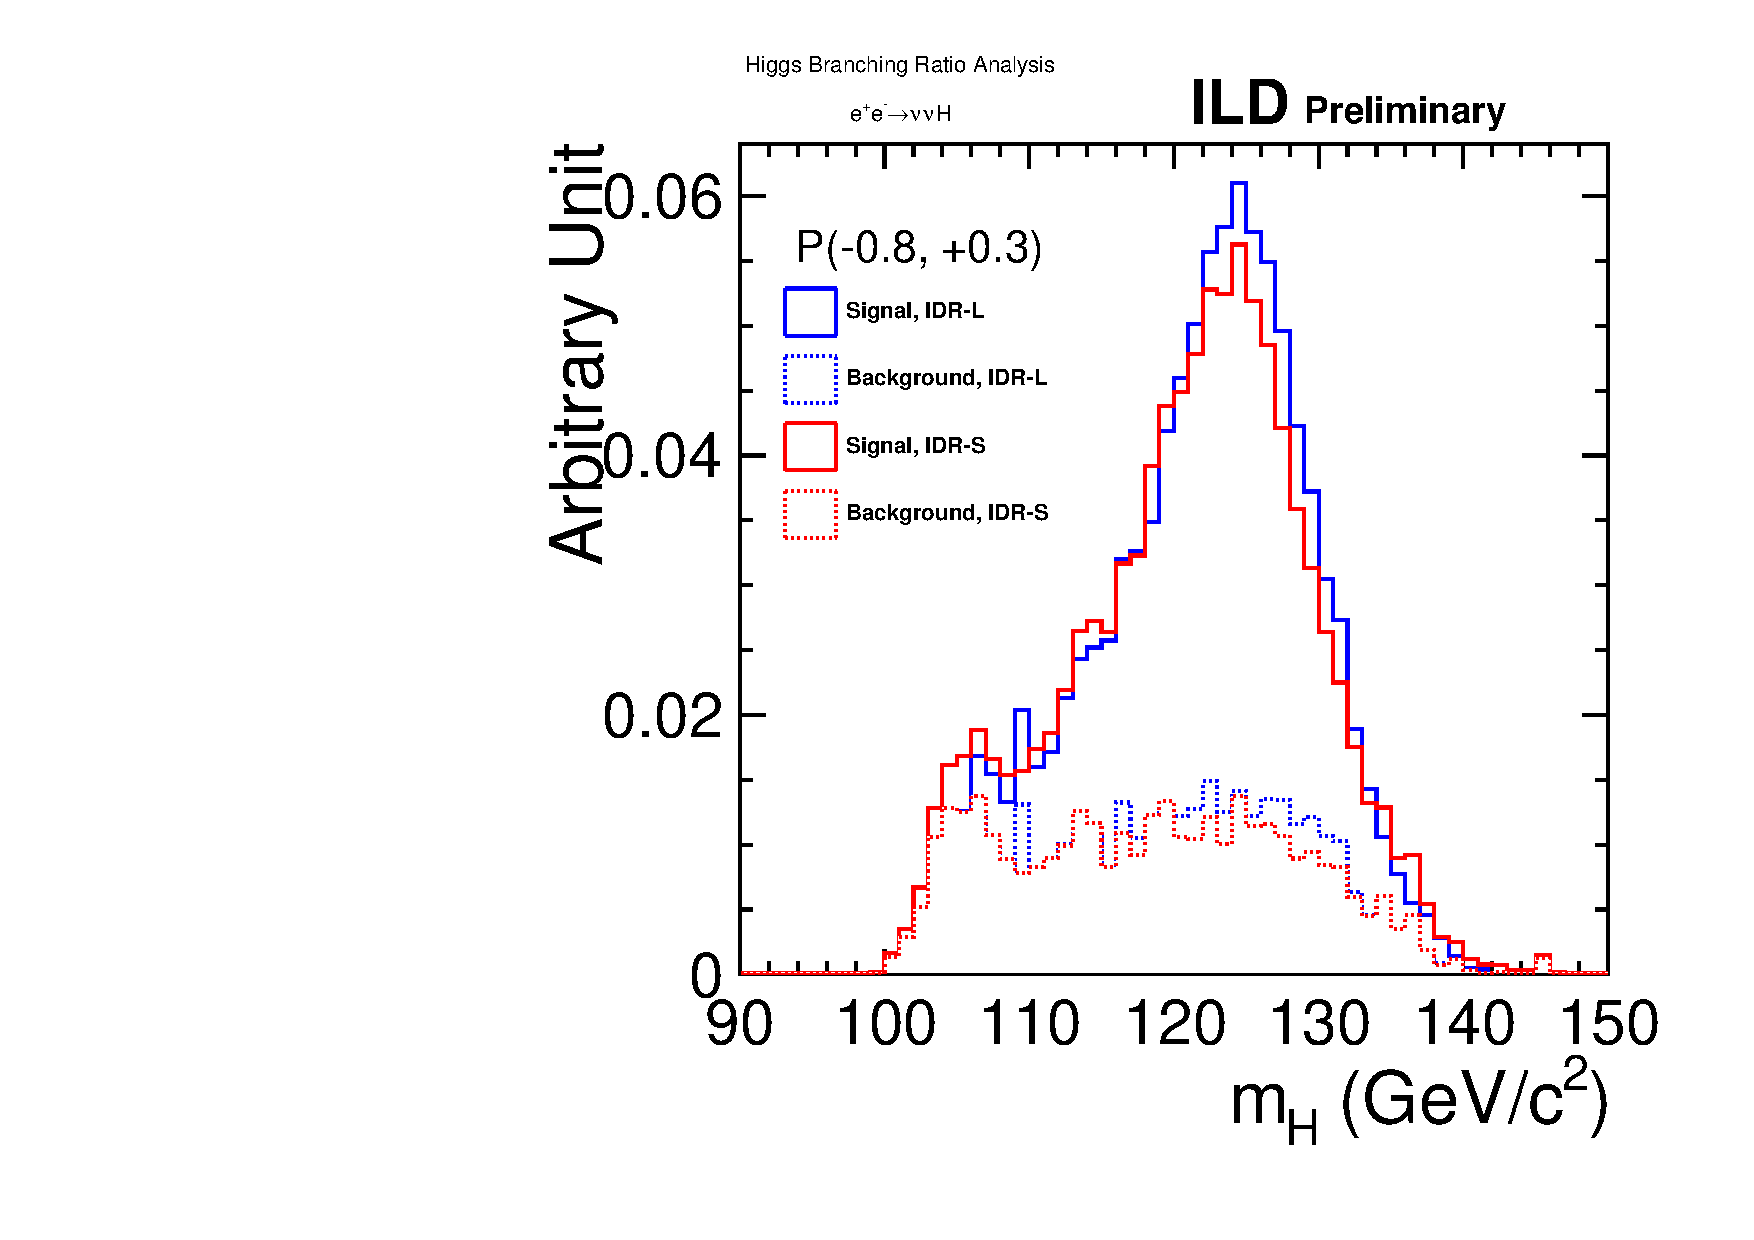
\includegraphics[width=0.5\textwidth]{Performance/fig/IDRplot5.pdf}
\end{center}
\caption{Reconstructed Higgs mass distribution after the kinematic selection. The signal is shown on top of the remaining SM background for the $P(e^-,e^+)=(-80\%,+30\%)$ data set of ILC500 as defined in Sec.~\ref{sec:benchmarks:lep}. The histograms have been normalized such that $S+B$ has an integral of $1$ in order to allow a better shape comparison between the two detector models.
}
\label{fig:Hbbccgg:mh}
\end{figure}


\begin{figure}[htbp]
\begin{center}
 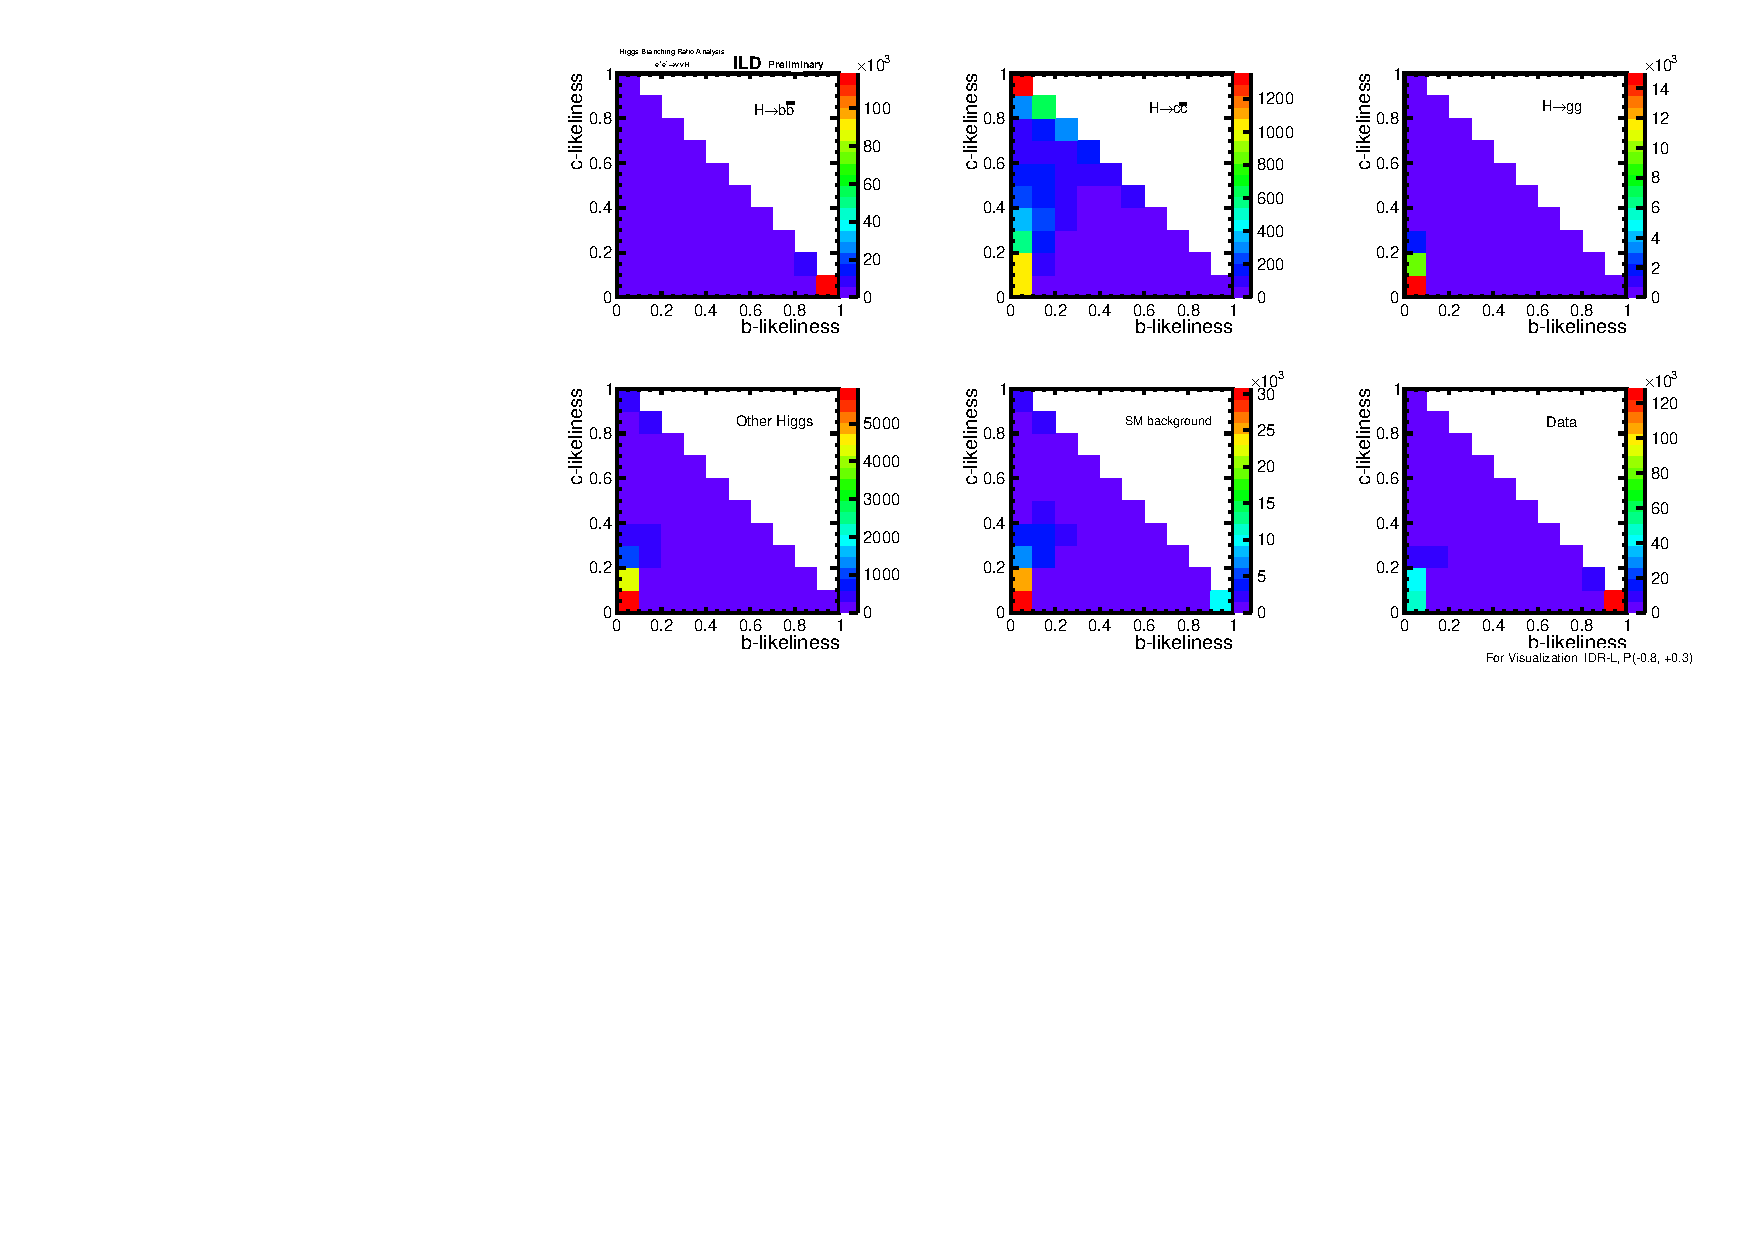
\includegraphics[width=\textwidth]{Performance/fig/IDRplot4.pdf}
\end{center}
\caption{Visualisation of the flavour tag performance in $\nu\bar{\nu} H$. The panels show the 2D distributions of $c$- vs $b$-likeliness separately for $H \to b\bar{b}$, $H \to c\bar{c}$, $H \to gg$, $H \to$other, the SM background and their mix expected in data for the $P(e^-,e^+)=(-80\%,+30\%)$ data set of ILC500 as defined in Sec.~\ref{sec:benchmarks:lep}.
}
\label{fig:Hbbccgg:likeli}
\end{figure}

Figure~\ref{fig:Hbbccgg:likeli} shows the 2D distributions of $c$- vs $b$-likeliness (c.f.\ Sec.~\ref{sec:perf:hlr:lcfi})for the different Higgs decay modes. The $x$-likeliness (for $x=c$, $b$ or $bc=c/(b+c)$) is obtained by combining the flavour tag output for the two individual jets, $x_1$ and $x_2$, according to
\begin{equation}
x = \frac{x_1 \cdot x_2}{(x_1\cdot x_2+(1-x_1)(1-x_2))}
\label{eqn:flavourtag}
\end{equation}
The ``data'' distribution is then fitted in 3D template approach in order to determine the contained fractions of the various hadronic Higgs decay modes, where the 3rd dimension is the $bc$-likeliness. Due to the limited available statistics of background MC, a much smaller number of bins than displayed in Fig.~\ref{fig:Hbbccgg:likeli} was used~\cite{ILDNote:Hbbccgg}. The resulting precisions from this template fit are displayed in Fig.~\ref{fig:Hbbccgg:BR}.  Fig.~\ref{fig:Hbbccgg:BR:cheat} shows the actual results for IDR-L and IDR-S with the $P(e^-,e^+)=(-80\%,+30\%)$ data only. For comparison,  the corresponding result obtained for a perfect flavour tag is also displayed. The comparison shows that for $H \to b\bar{b}$ and $H \to gg$, the current flavour tag performance yields a close to perfect identification of these final states. For $H \to c\bar{c}$, however, the
real flavour tag performs worse by a factor of two. On the other hand, for a worse flavour separation, especially the expected precision for $H \to c\bar{c}$ degrades rapidly~\cite{ILDNote:Hbbccgg},
thus the performance of the ILD detector and reconstruction is crucial for the ability to measure $H \to c\bar{c}$.

Figure~\ref{fig:Hbbccgg:BR:LS} finally compares for IDR-L and IDR-S the precisions combined over all data sets of ILC500 as defined in Sec.~\ref{sec:benchmarks:lep}. It shows a rather equivalent performance of both detector models. In the case of $H \to c\bar{c}$, which is most sensitive to the detector performance, the smaller detector model actually performs a little better: Due to the stronger magnetic field of IDR-S, less tracks from $\gamma\gamma \to$ low-$p_t$ hadron overlay are reconstructed, which helps the charm tag to perform a bit better. 


\begin{figure}[htbp]
%\begin{center}
\begin{subfigure}{0.49\hsize} 
 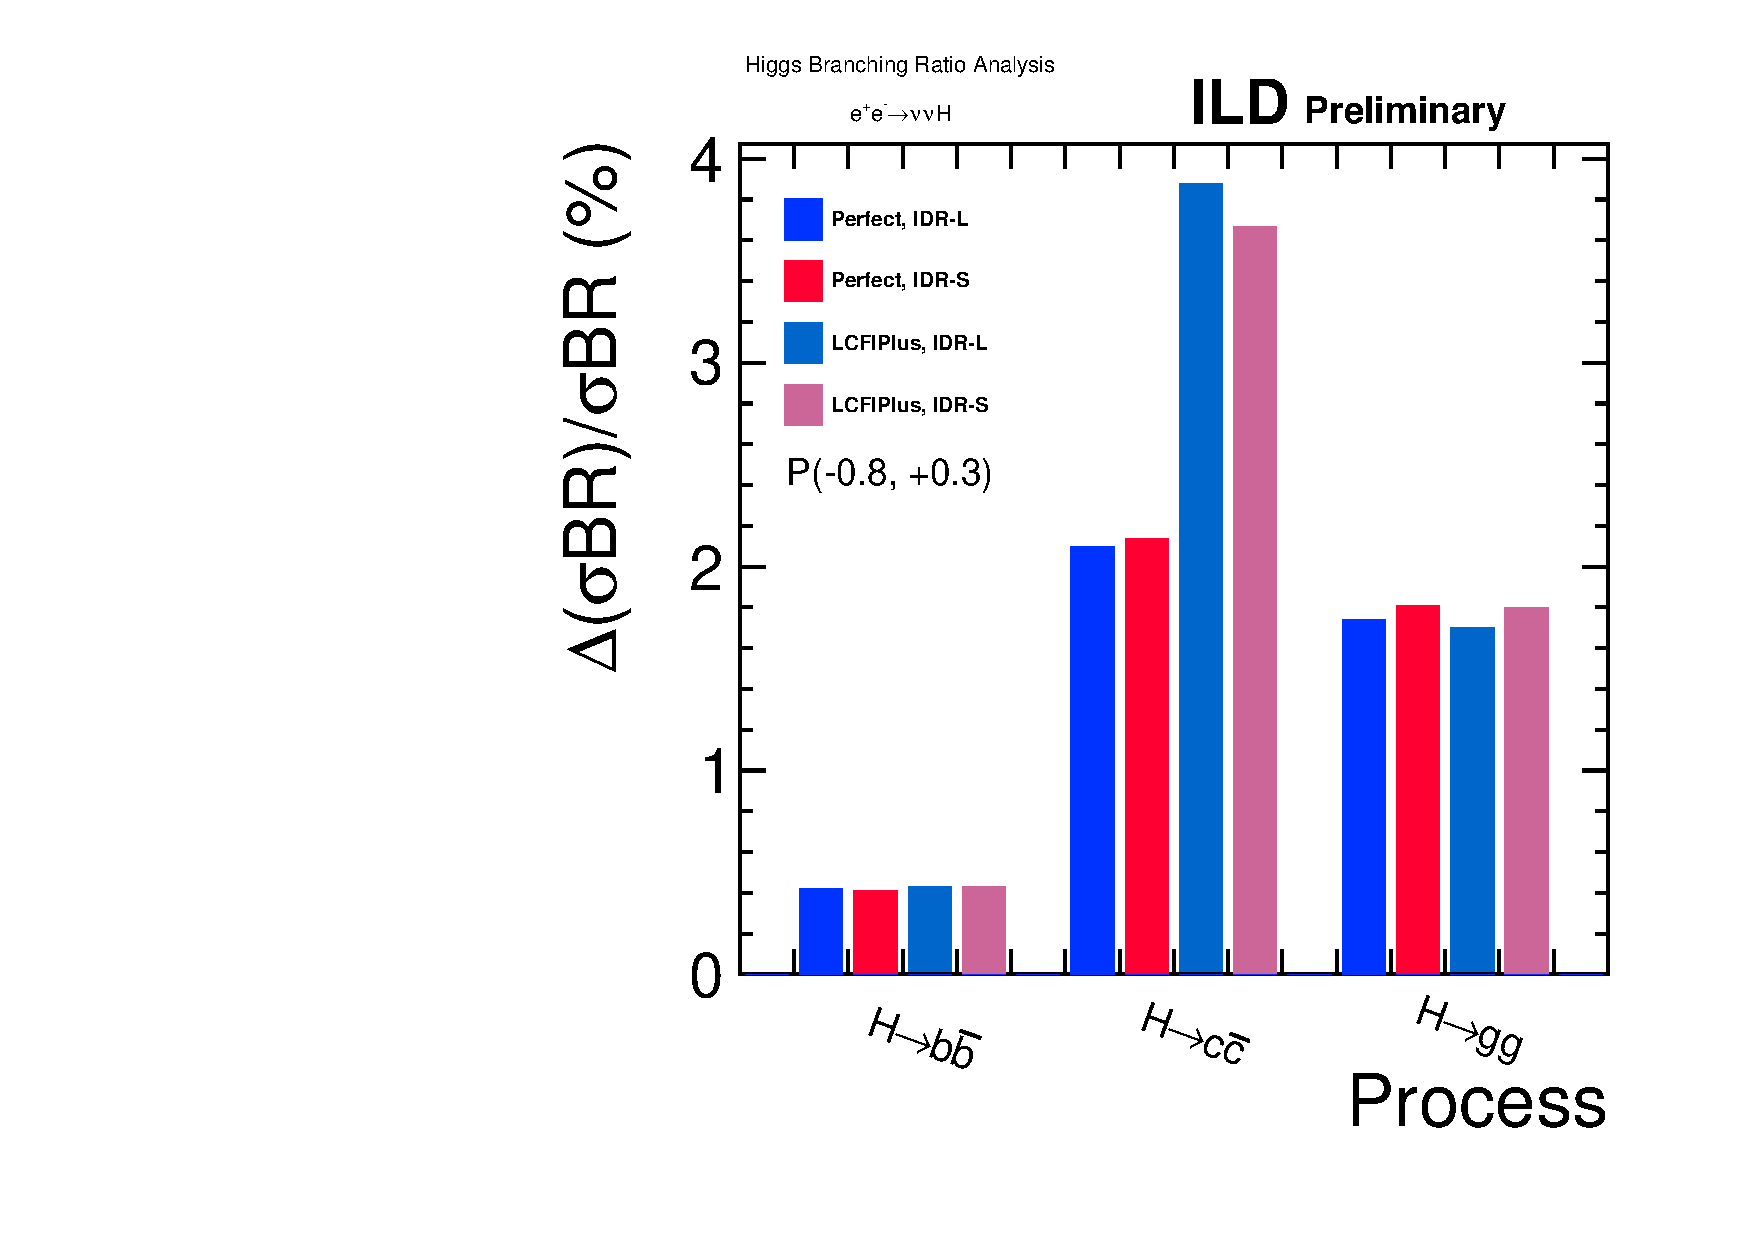
\includegraphics[width=\textwidth]{Performance/fig/IDRplot1.pdf}
 \caption{ \label{fig:Hbbccgg:BR:cheat}}
 \end{subfigure}
%\hspace{0.03\textwidth}
\begin{subfigure}{0.49\hsize} 
 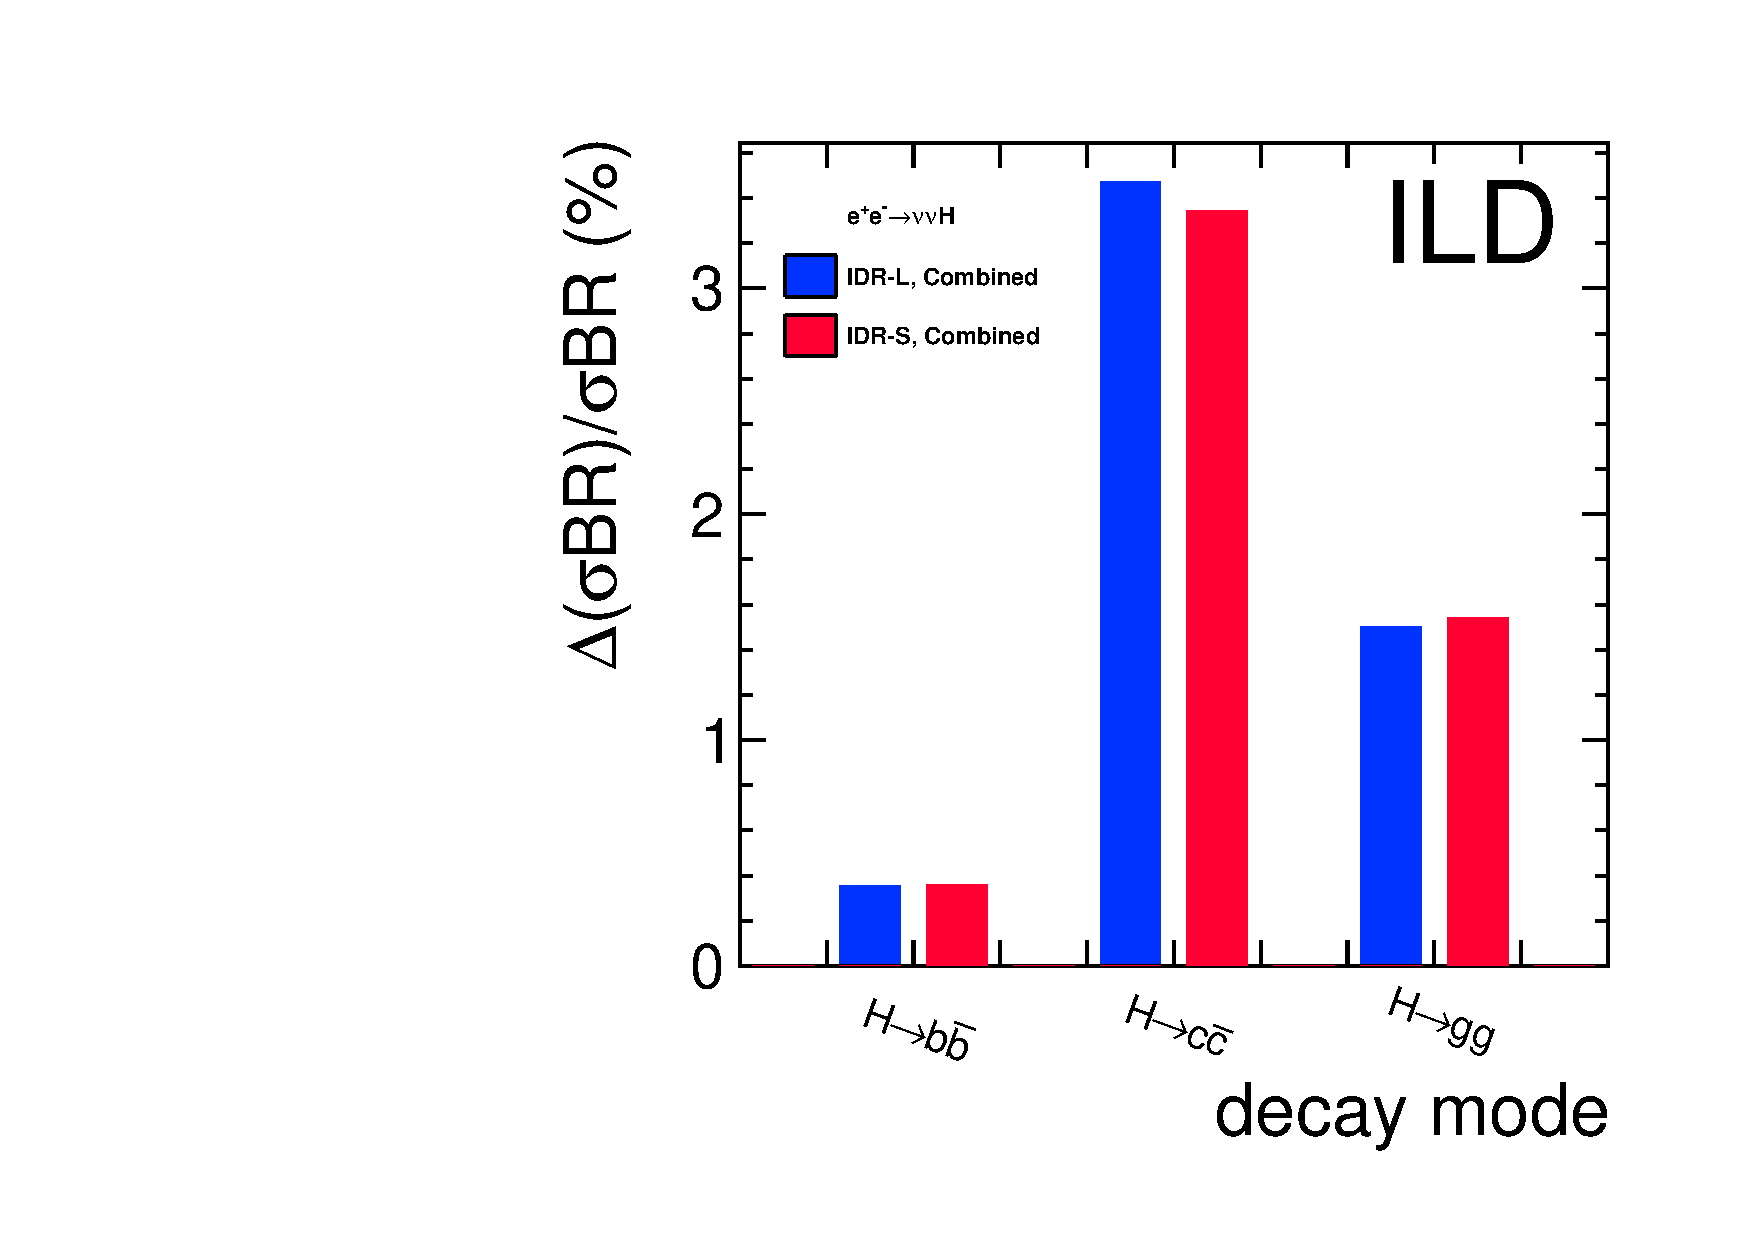
\includegraphics[width=\textwidth]{Performance/fig/IDRplot3.pdf}
 \caption{  \label{fig:Hbbccgg:BR:LS}}
 \end{subfigure}
%\end{center}
\caption{
(a) Comparison of current and ideal flavour tag performance for the $P(e^-,e^+)=(-80\%,+30\%)$ data set of ILC500 as defined in Sec.~\ref{sec:benchmarks:lep}. The precision on $H \to c\bar{c}$ is most sensitive to the actual flavour tag performance.
(b) Comparison of IRD-L and IDR-S for all polarisation configurations of ILC500 as defined in Sec.~\ref{sec:benchmarks:lep} combined.
}
\label{fig:Hbbccgg:BR}
\end{figure}

%%%%%%%%%%%%%%%%%%%%%%%%%%%%%%%%%%%%%%%%%%%%%%%%%%%%%%%%%%%%%%%%%%%
\subsection{Higgs Mass from \texorpdfstring{$ZH \to ll b\bar{b}$}{ZH -> llbb}}

The single most precise method to measure the Higgs mass is the recoil analysis at $\sqrt{s}=250$\,GeV~\cite{Yan:2016xyx}, for which a precision of $14$\,MeV has been projected for the full ILC250 data set~\cite{Fujii:2017vwa}. At $\sqrt{s}$ much higher than the $ZH$ production threshold, the recoil
technique suffers substantially from the increasing amount of ISR and beamstrahlung. In addition, the momenta of the muons from $Z\to \mu\mu$ increase in magnitude and thus are measured less precisely. Still, the data collected at higher centre-of-mass energies can be exploited effectively when using the fully-reconstructable decay modes of the Higgs boson in combination with kinematic constraints\footnote{In $x$ direction the initial momentum is not zero due to the crossing angle of the beams, but given by $\sqrt{s} \cdot \sin{14\,\mathrm{mrad}}$.} from the known initial state. E.g.\ the constraints $\sum_i{p_{i_y}}=0$ and $\sum_i{p_{i_x}}=3.5$\,GeV can replace the measured energies of the Higgs decay products, so that only the {\it angles} of the Higgs decay products and the momenta of the muons from $Z\to\mu^+\mu^-$ enter in the mass reconstruction. Thus the technique is independent of systematic uncertainties as e.g.\ associated with the $b$-jet energy scale. The detailed description of the technique can be found in~\cite{ILDNote:MH}.

The resolutions on the kinematic quantities which enter the Higgs mass reconstruction, namely azimuthal and polar angles of the jets and the muon energy, are compared in Figs.~\ref{fig:mh:res:phi_LS} and~\ref{fig:mh:res:etheta} for IDR-L and IDR-S. For this, 
the jet angles obtained from clustering the MC particles after hadronisation serve as truth reference, so that the detector performance is singled out from other influences.  Figure~\ref{fig:mh:res:phi_hadronisation} illustrates the effect of hadronisation by comparing to the quark-level direction taking IDR-L as example. It shows that the detector resolution (blue histogram, same as in Fig.~\ref{fig:mh:res:phi_LS}) is comparable, but
smaller than the hadronisation effect (red histogram). While the angular resolutions are very similar for both detector models, the muon energy resolution is worse for the small detector, reflecting the somewhat worse $p_t$ resolution for high-momentum tracks in the central region of the detector, c.f.\ Fig.~\ref{fig:perf:trkres}. 
 
\begin{figure}[htbp]
%\begin{center}
\begin{subfigure}{0.49\hsize} 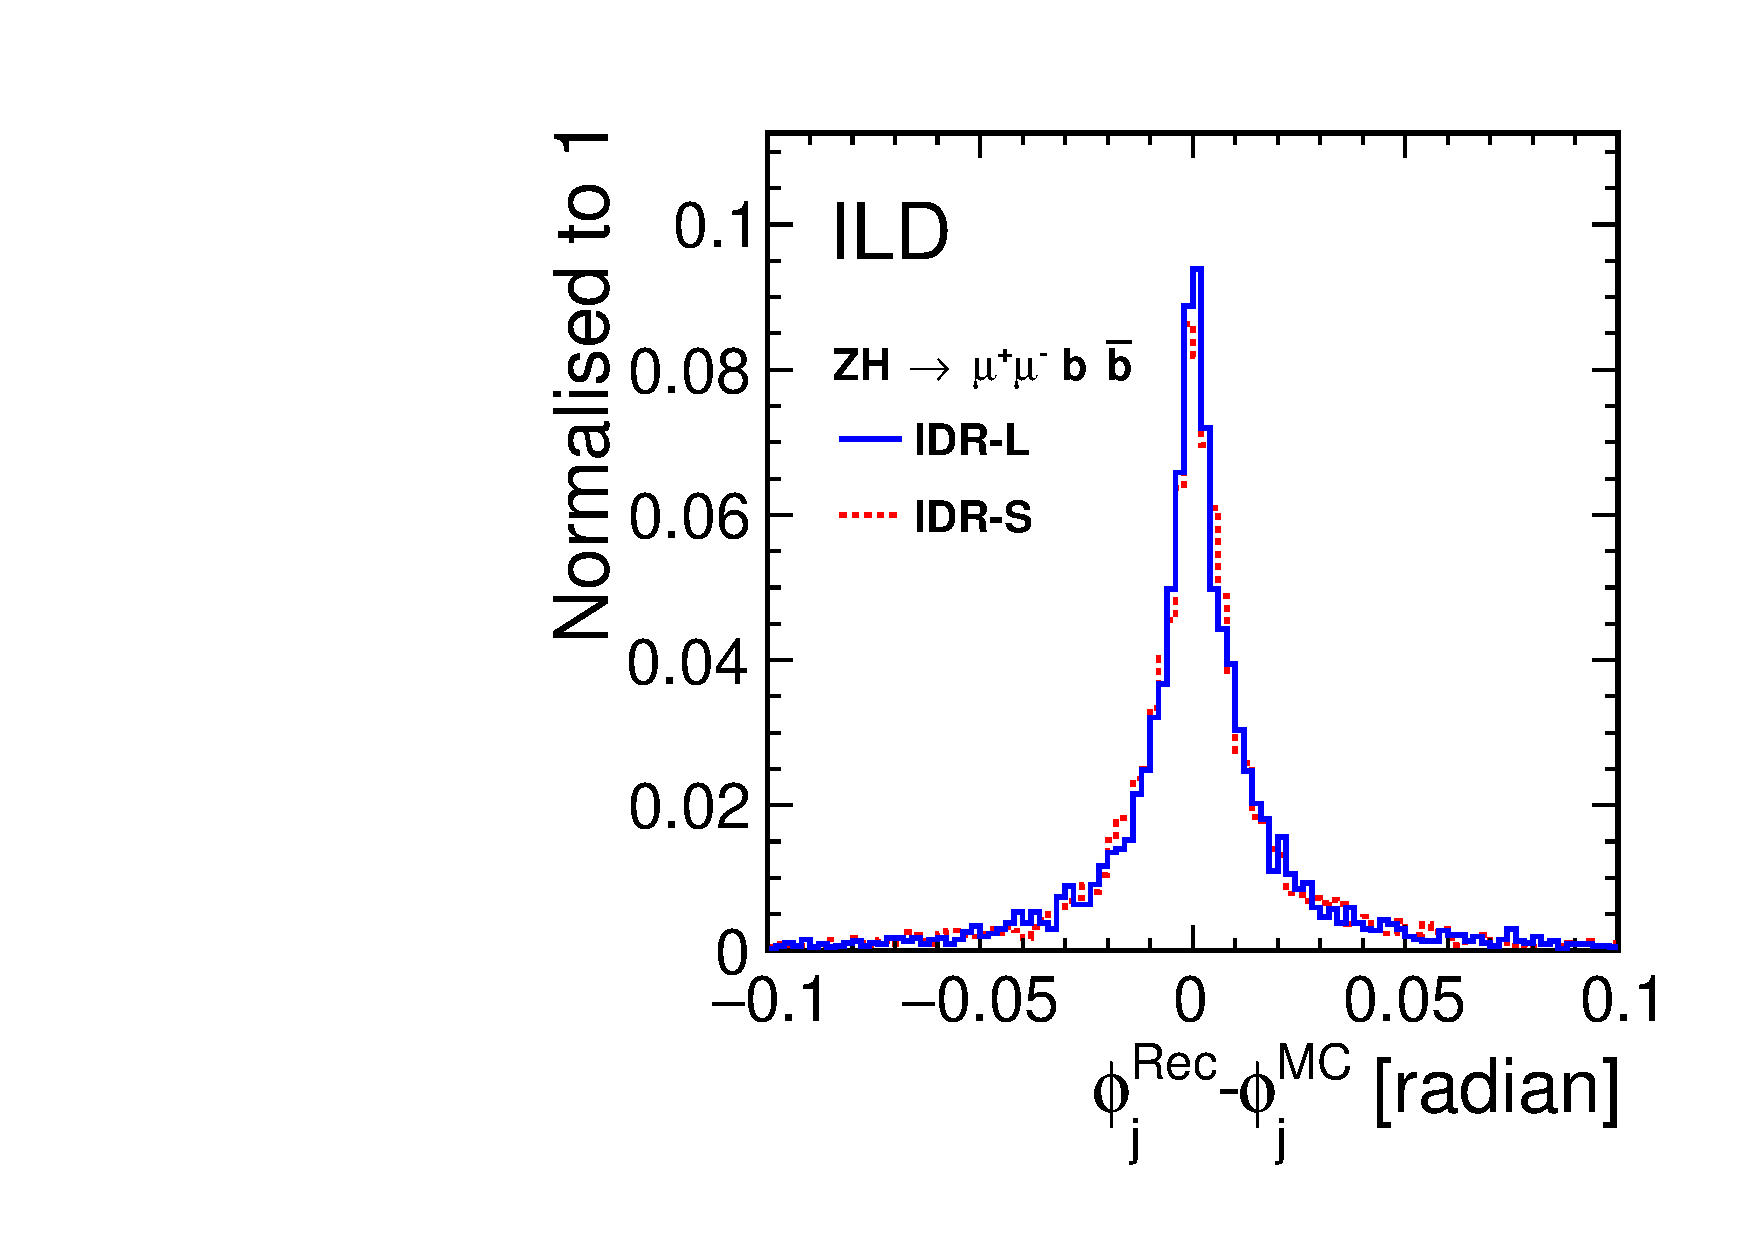
\includegraphics[width=\textwidth]{Performance/fig/phij1h.pdf}
 \caption{ \label{fig:mh:res:phi_LS}}
 \end{subfigure}
%\hspace{0.03\textwidth}
\begin{subfigure}{0.49\hsize} 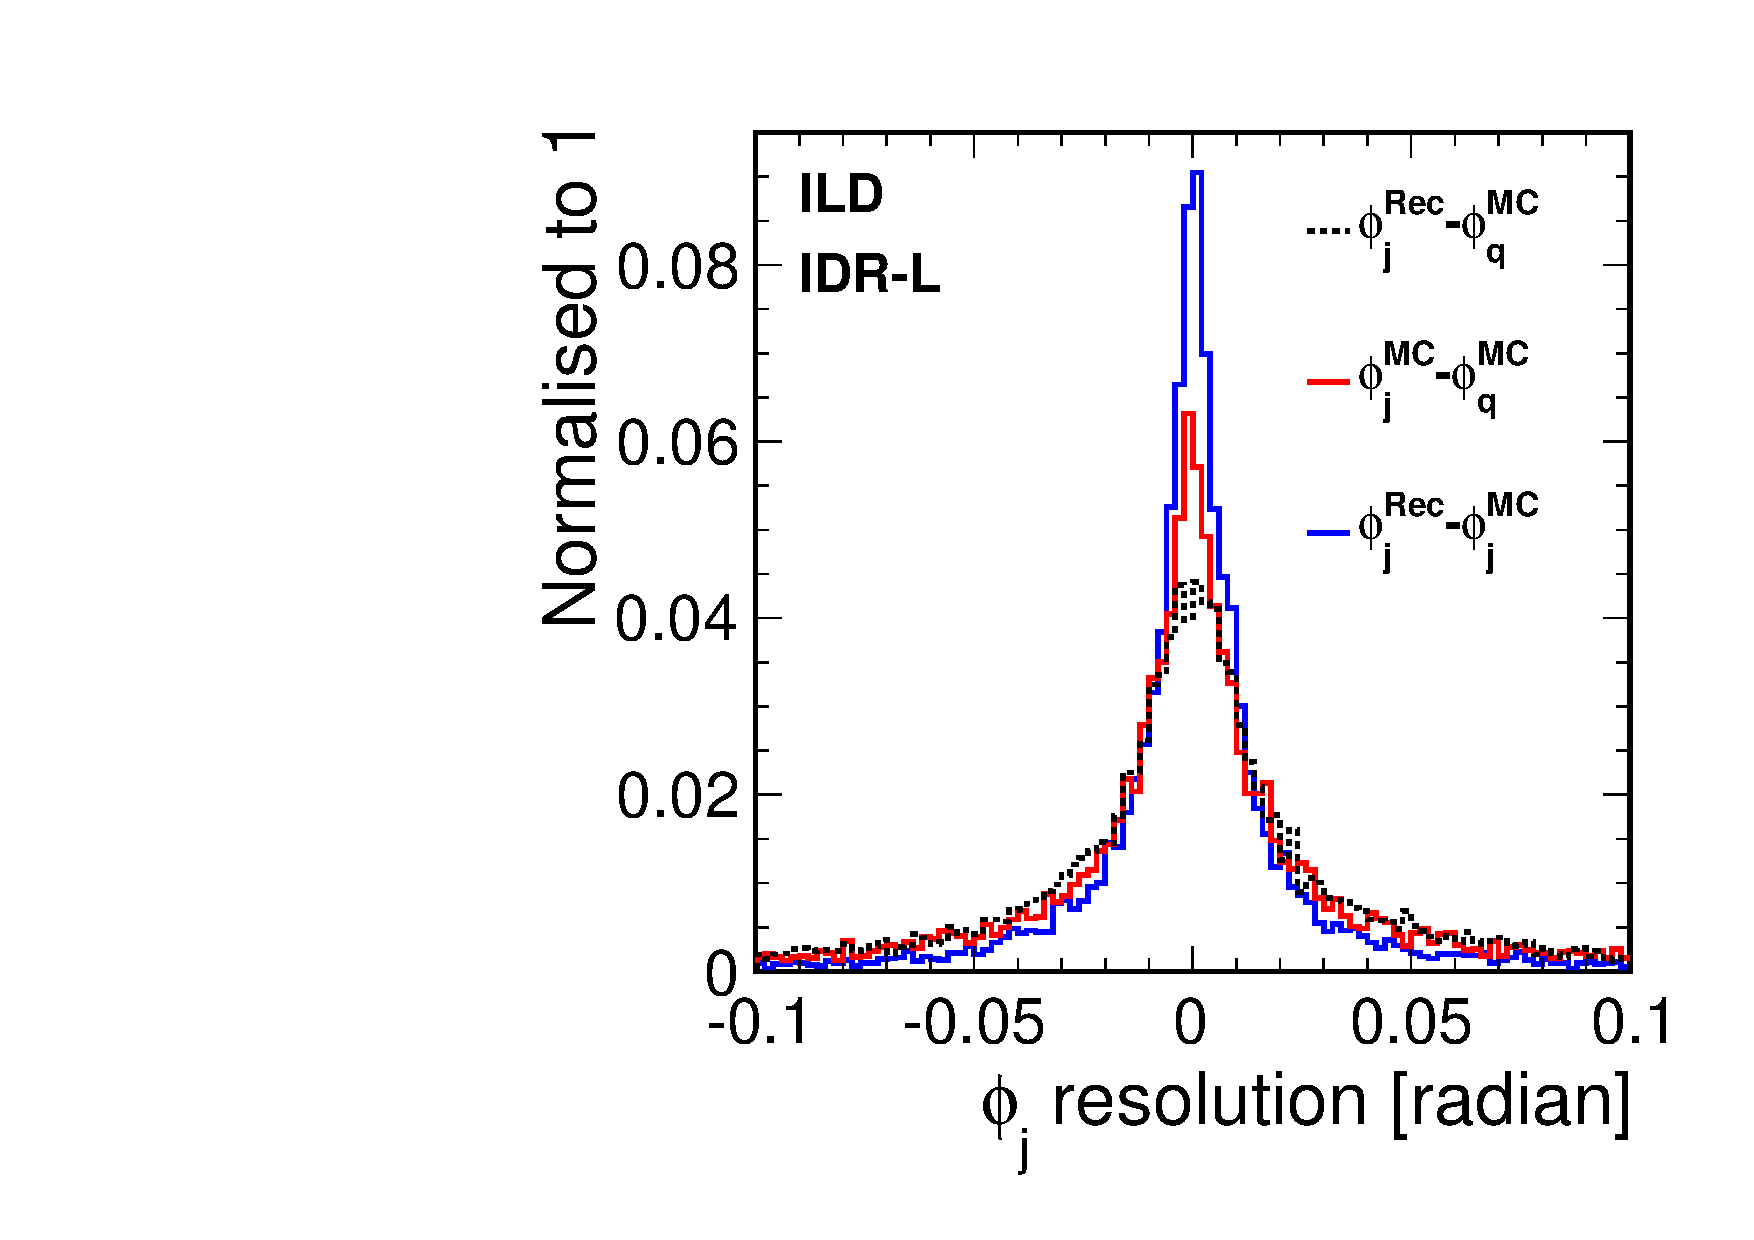
\includegraphics[width=\textwidth]{Performance/fig/phi_res.pdf}
 \caption{  \label{fig:mh:res:phi_hadronisation}}
 \end{subfigure}
%\end{center}
\caption{Reconstruction of the jet azimuthal angle in $ZH \to \mu^+ \mu^- b\bar{b}$: 
(a) Resolution obtained with IDR-L and IDR-S for the jet azimuthal angle
(b) Influence of hadronisation on the jet azimuthal angle
}
\label{fig:mh:res:phi}
\end{figure}

\begin{figure}[htbp]
%\begin{center}
\begin{subfigure}{0.49\hsize} 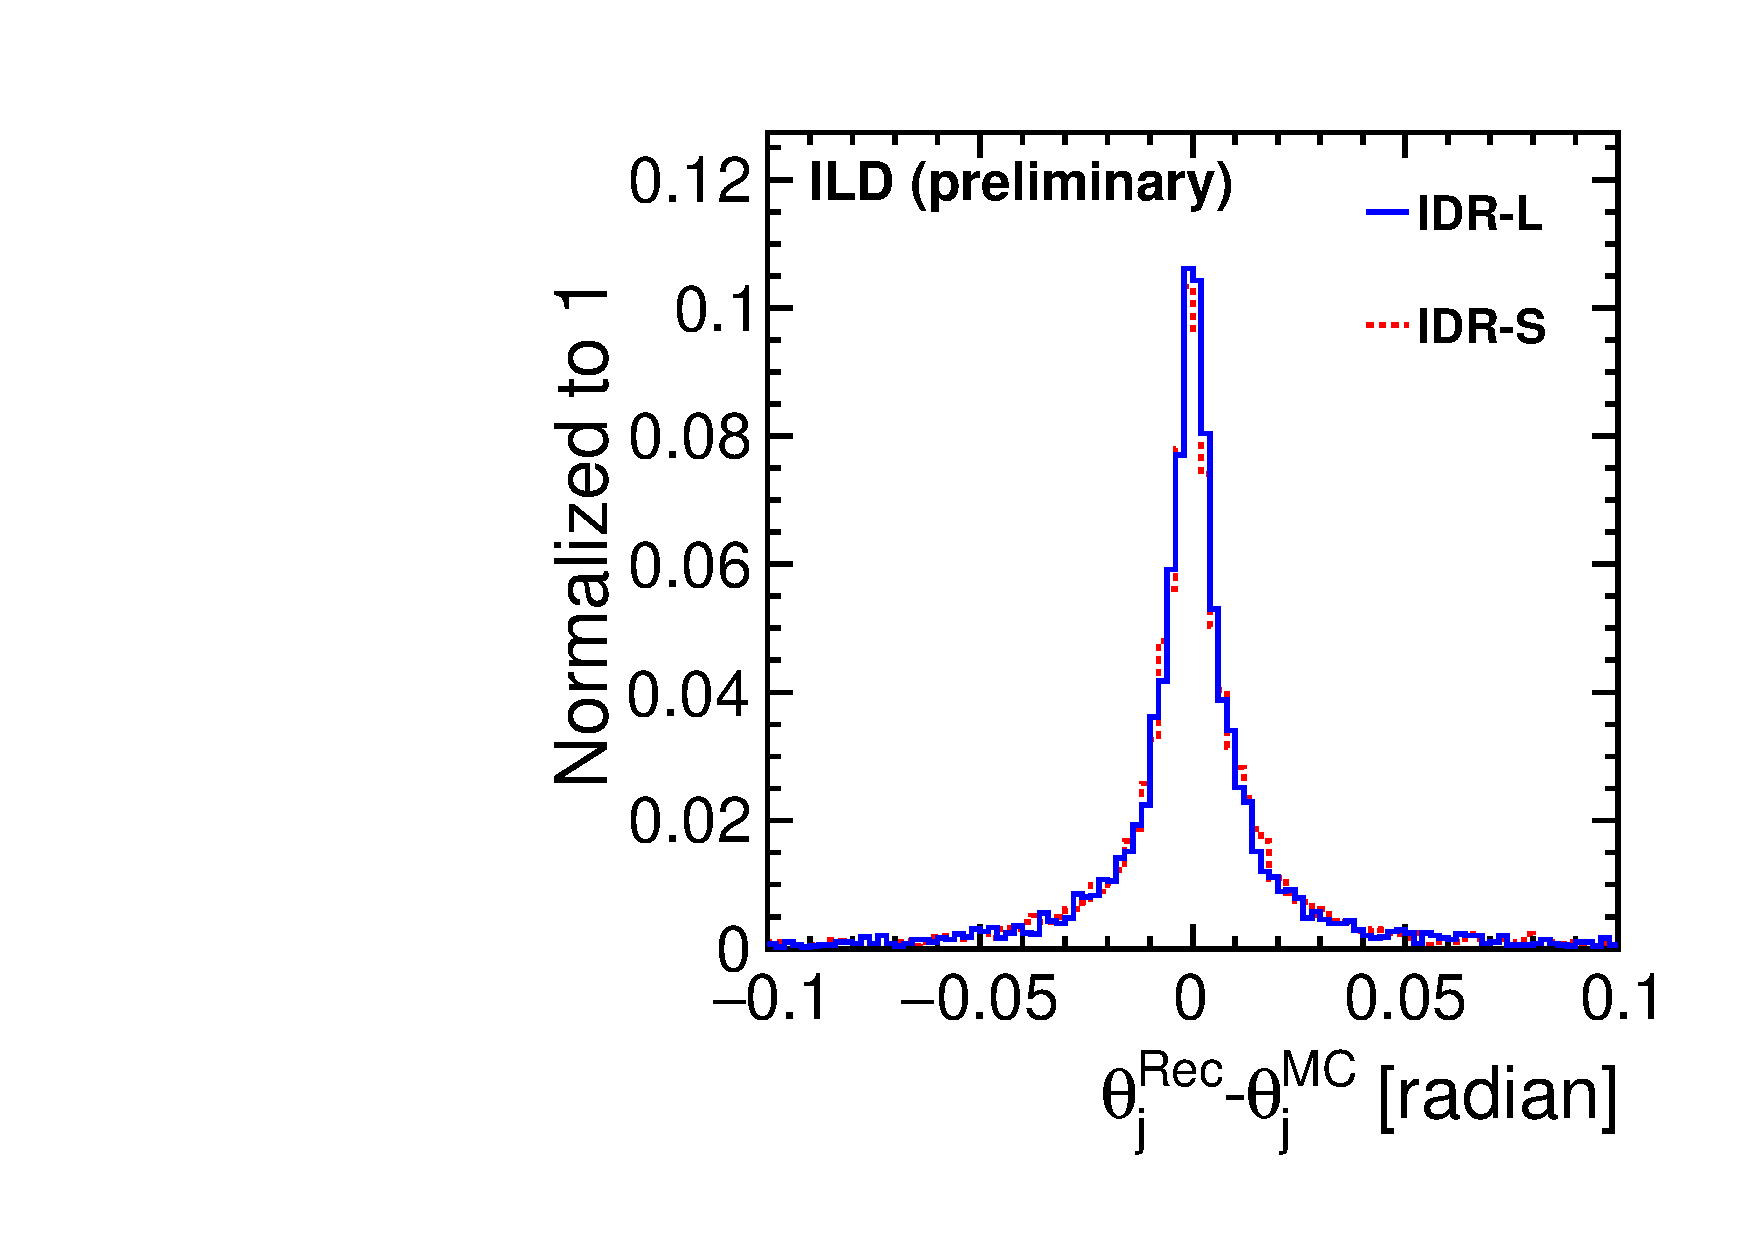
\includegraphics[width=\textwidth]{Performance/fig/thetaj1h.pdf}
 \caption{  \label{fig:mh:res:theta}}
 \end{subfigure}
%\hspace{0.03\textwidth}
\begin{subfigure}{0.49\hsize} 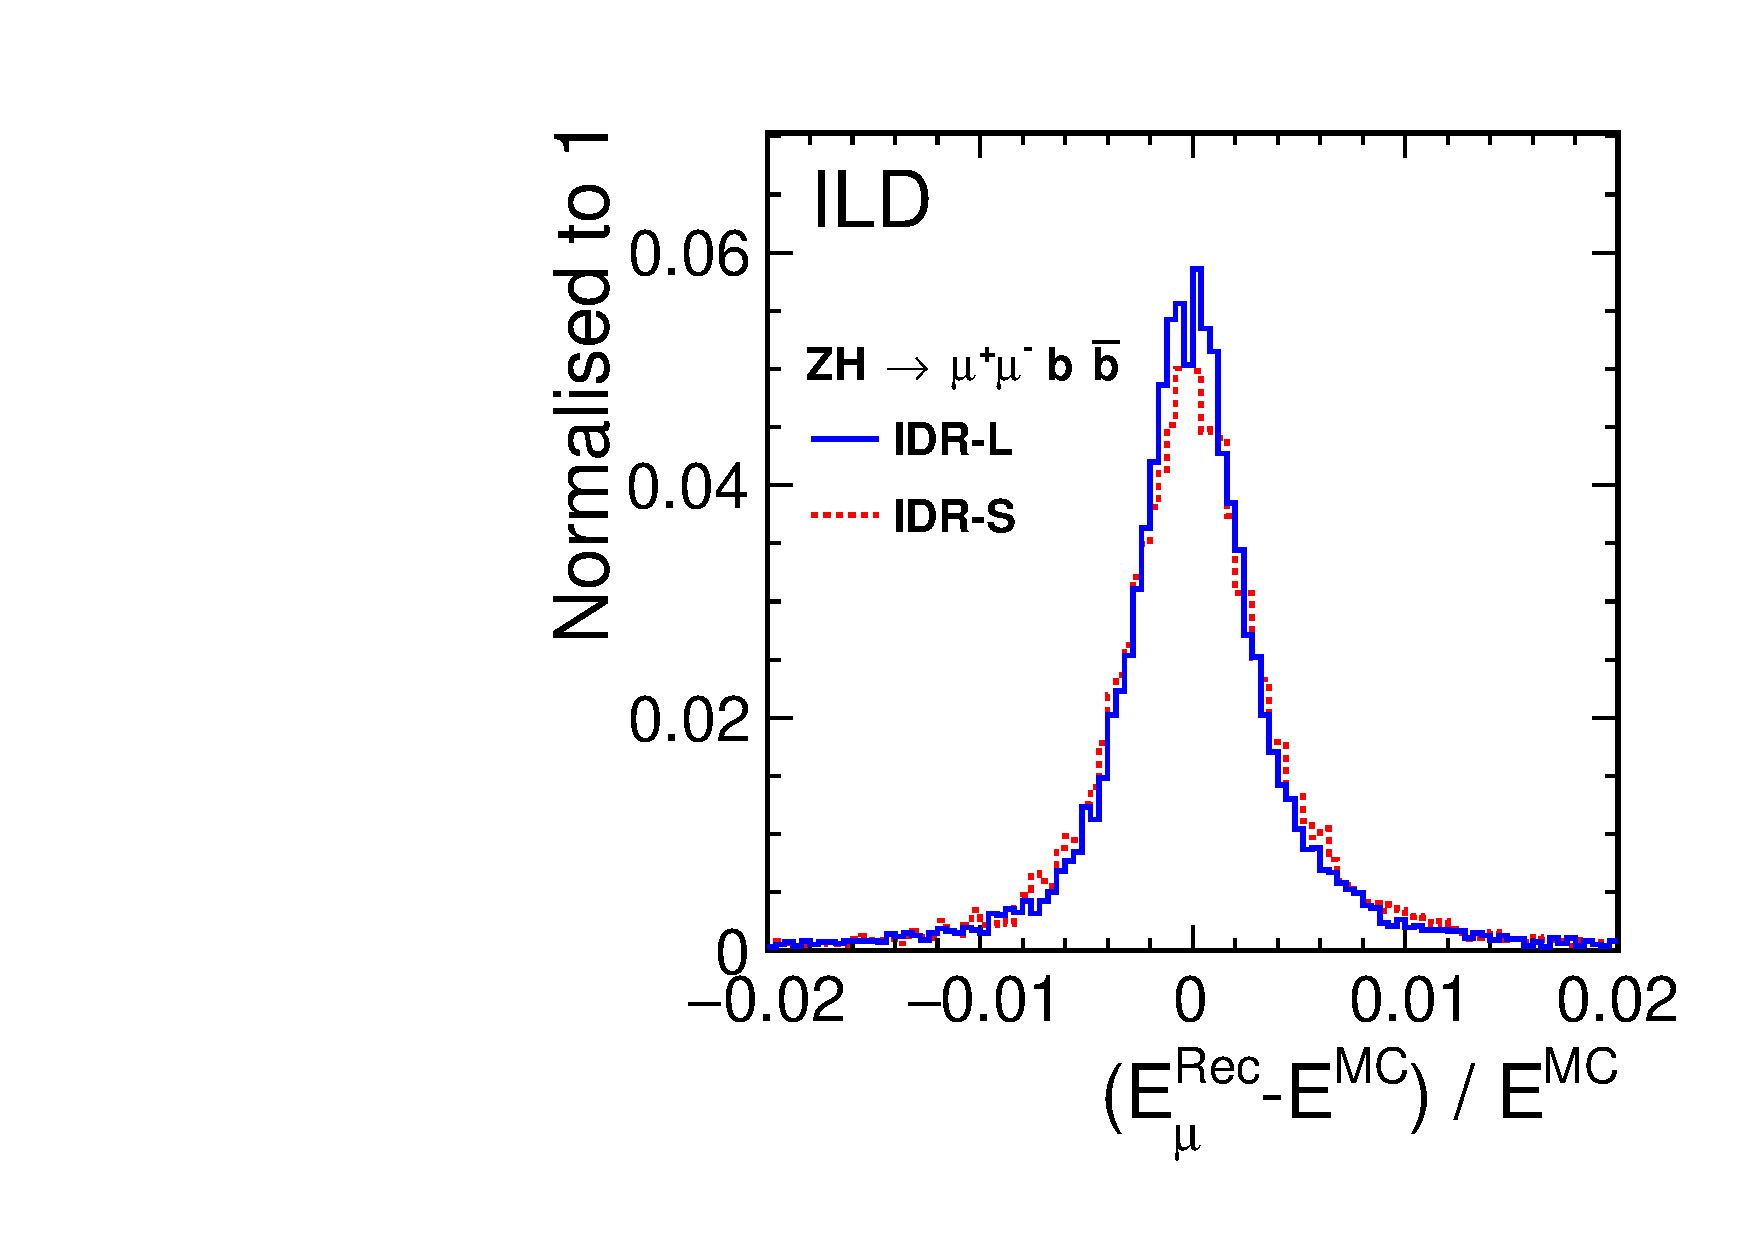
\includegraphics[width=\textwidth]{Performance/fig/elep1.pdf}
 \caption{  \label{fig:mh:res:Elep}}
 \end{subfigure}
%\end{center}
\caption{Resolutions obtained  in $ZH \to \mu^+ \mu^- b\bar{b}$ with IDR-L and IDR-S for 
(a) the jet polar angle
(b) the muon energy, after recovery of FSR photons. 
}
\label{fig:mh:res:etheta}
\end{figure}

Figure~\ref{fig:mh:mass} shows the propagation of this effect to the actual physics observable, i.e.\ the reconstructed mass of the Higgs candidates. IDR-L and IDR-S are compared for the muon channel in Fig.~\ref{fig:mh:mass:mumu} and for the electron channel in Fig.~\ref{fig:mh:mass:ee}. In both cases signal and all backgrounds from the SM and other $ZH$ modes are combined, with clear peaks visible around the nominal Higgs and $Z$ boson masses. In particular in the muon channel, the worse momentum resolution of the small detector leads to the peaks being visibly wider. The uncertainty on the Higgs mass is extracted by fitting these distributions following the approach used for the recoil analysis~\cite{Yan:2016xyx}. For ILC500 as defined in Sec.~\ref{sec:benchmarks:lep}, this results in an uncertainty on the measured Higgs mass of $66$\,MeV in the case of IDR-L and $81$\,MeV for IDR-S, an increase of about $22\%$.

\begin{figure}[htbp]
%\begin{center}
\begin{subfigure}{0.49\hsize} 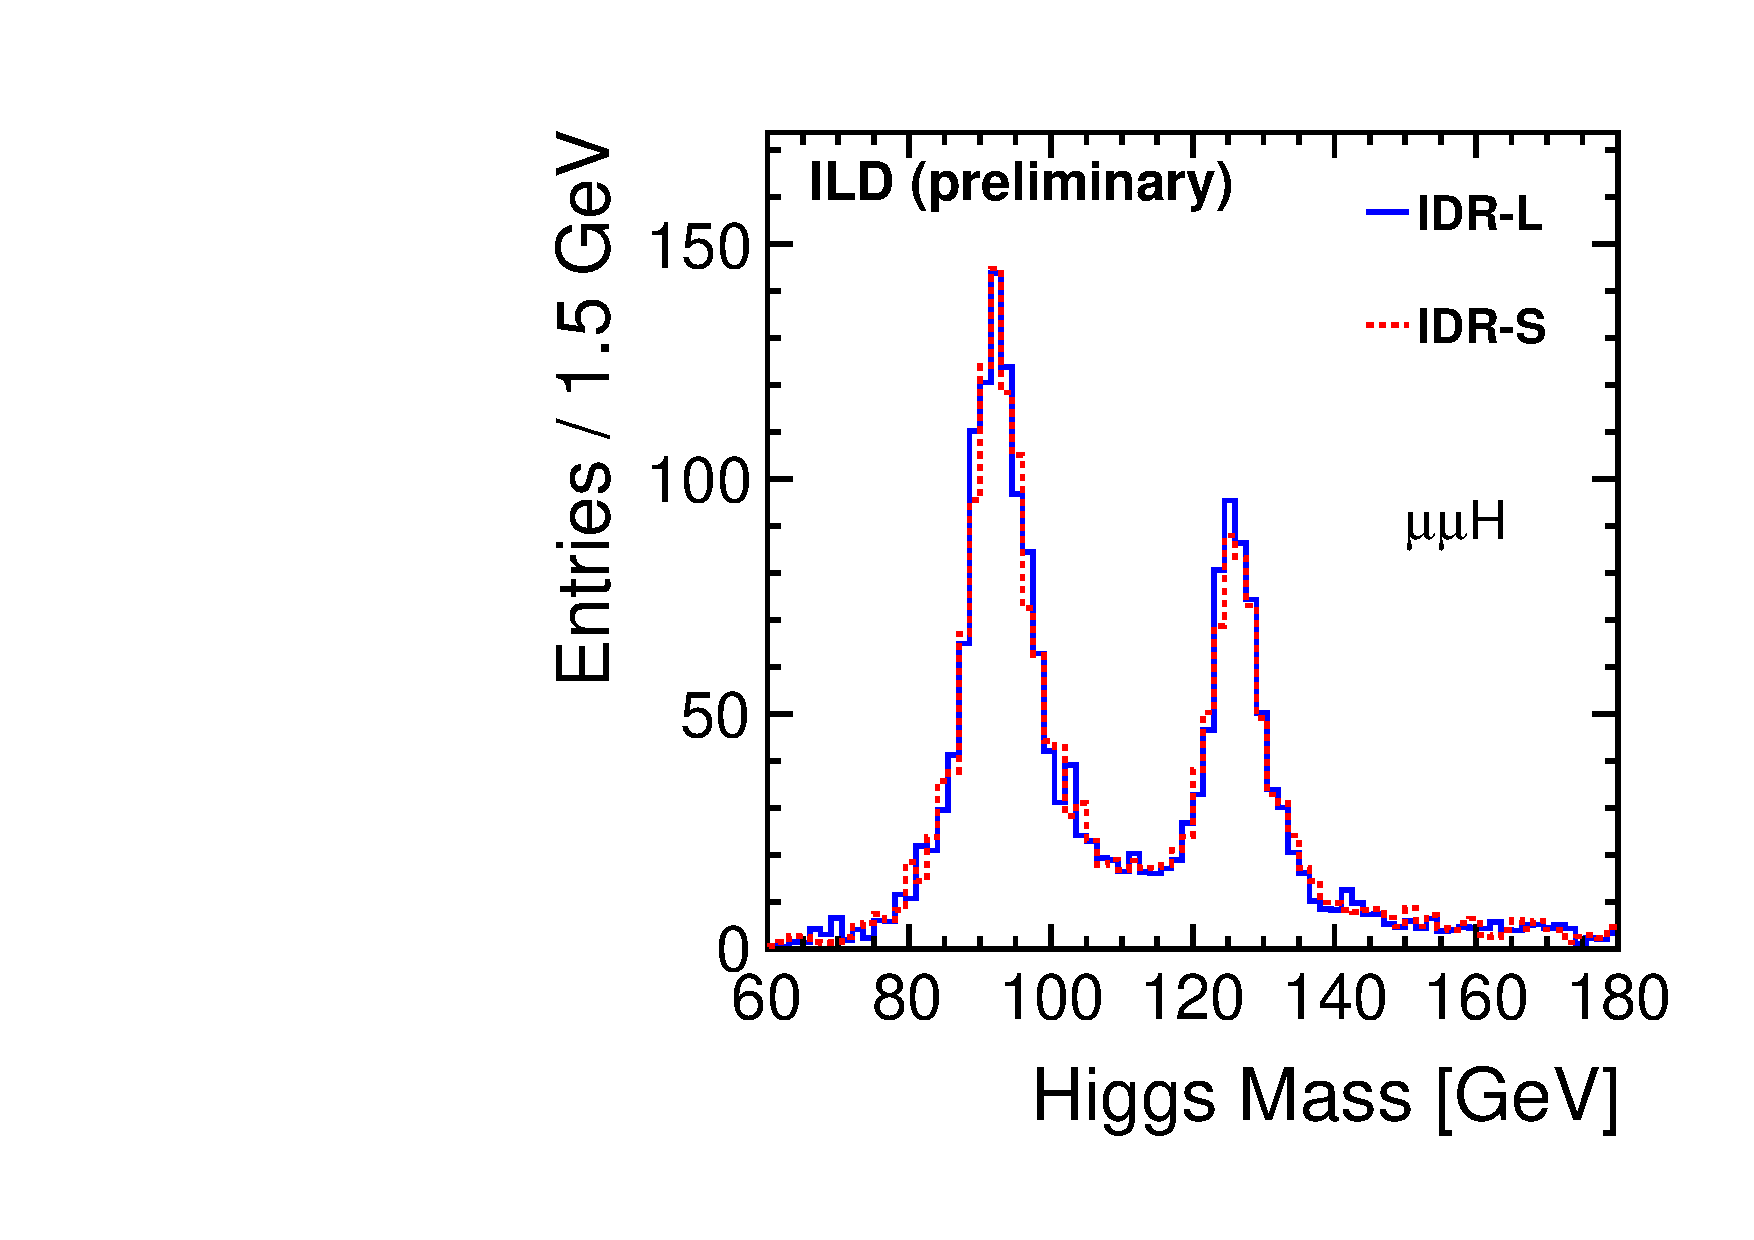
\includegraphics[width=\textwidth]{Performance/fig/mH_e2e2h_bb_eLpR_IDR.pdf}
 \caption{ \label{fig:mh:mass:mumu}}
 \end{subfigure}
%\hspace{0.03\textwidth}
\begin{subfigure}{0.49\hsize} 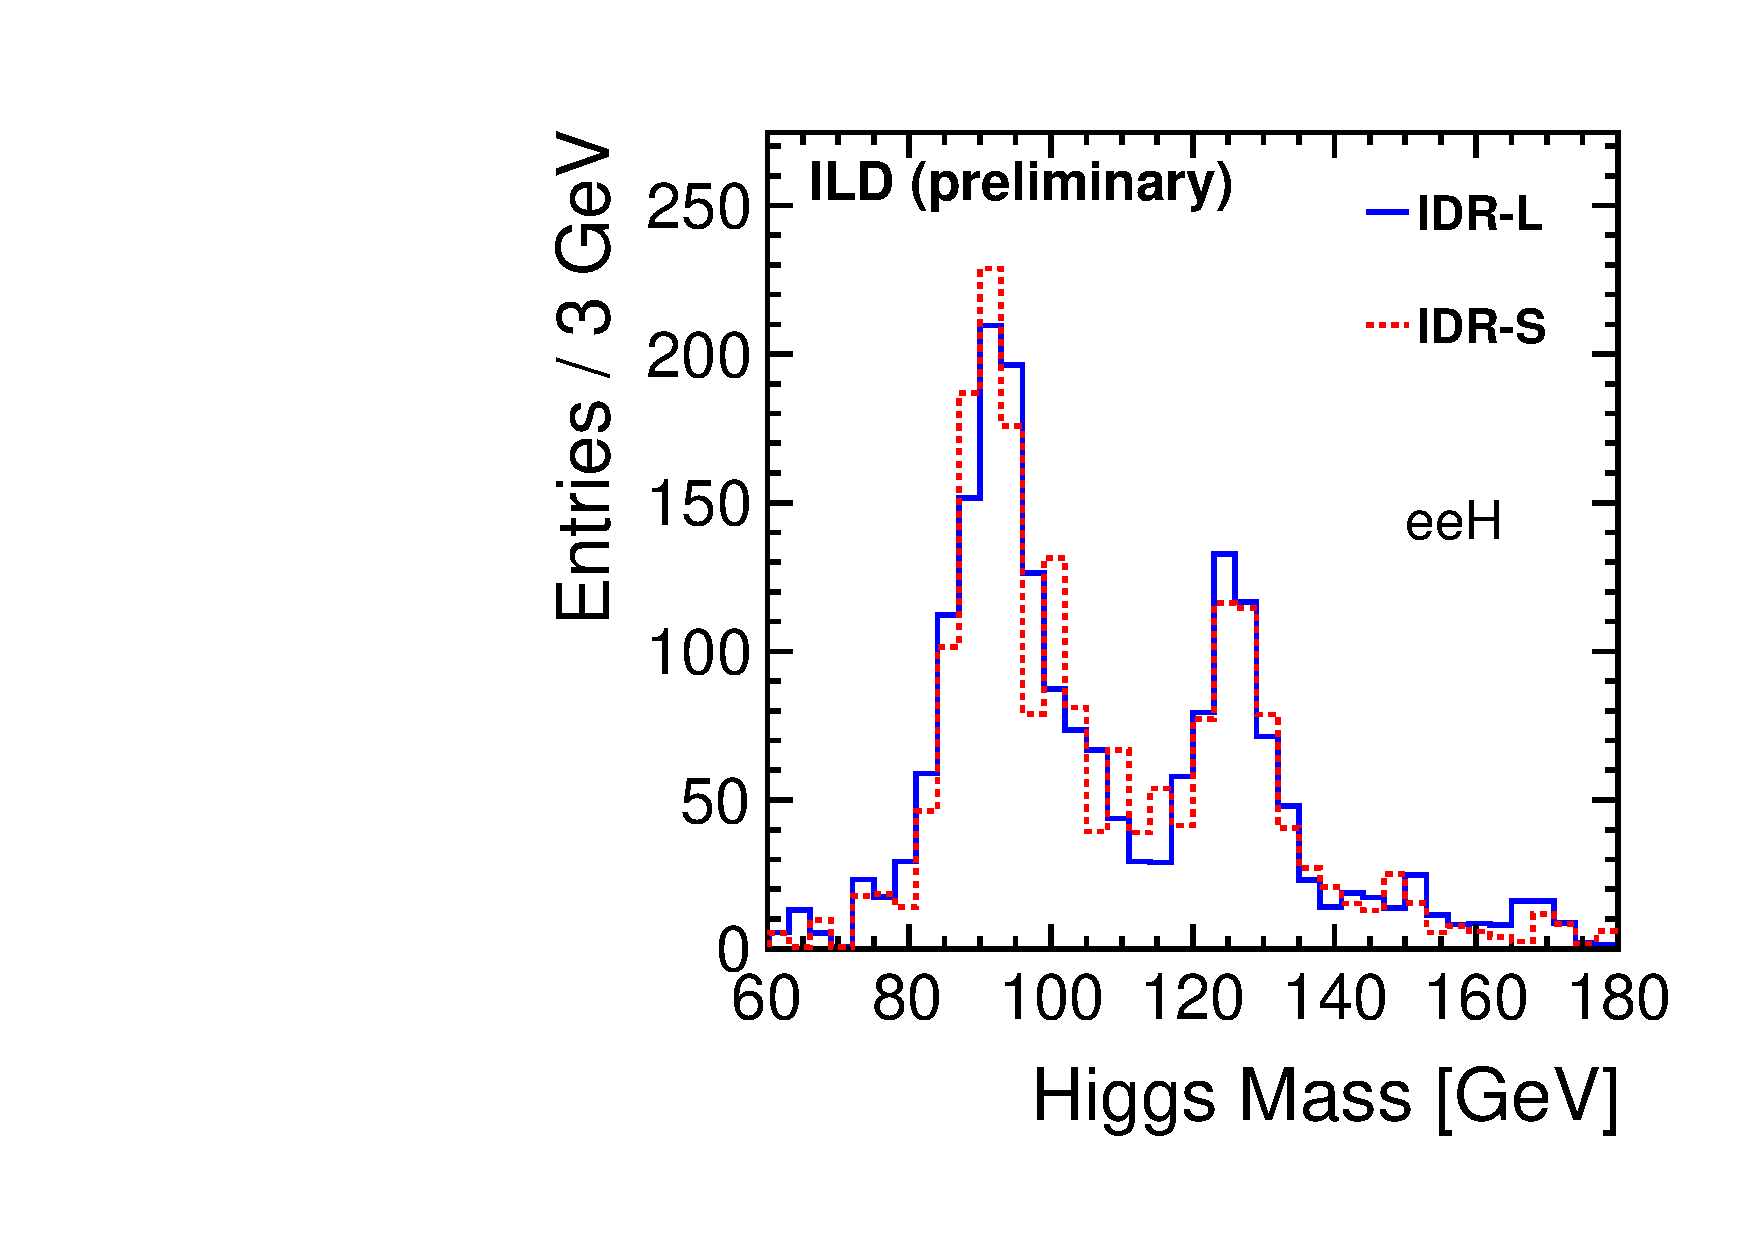
\includegraphics[width=\textwidth]{Performance/fig/mH_e1e1h_bb_eLpR_IDR.pdf}
 \caption{  \label{fig:mh:mass:ee}}
 \end{subfigure}
%\end{center}
\caption{Reconstructed Higgs mass distribution in $ZH \to l^+ l^- b\bar{b}$ for signal and background for IDR-L and IDR-S at ILC500 as defined in Sec.~\ref{sec:benchmarks:lep} for
(a) the muon channel
(b) the electron channel (here with limited MC statistics, thus a reduced number of bins)
}
\label{fig:mh:mass}
\end{figure}


%%%%%%%%%%%%%%%%%%%%%%%%%%%%%%%%%%%%%%%%%%%%%%%%%%%%%%%%%%%%%%%%%%%
\subsection{Branching Ratio of \texorpdfstring{$H \to \mu^+\mu^-$}{H -> mm}}

In the SM, the decay of the Higgs boson into a pair of muons is a very rare decay, with a branching ratio of $2.2 \times 10^{-4}$. In order to identify this small signal, the achievable mass resolution, thus the precision to which the momenta of the two muons are measured, plays a crucial role. For the purpose of detector benchmarking, we consider only 
$\sigma(\nu\bar{\nu} H)\times BR(H\to \mu^+\mu^-)$ as observable, which isolates best the effect of the muon momentum resolution. At center-of-mass energies above $350$\,GeV, the $\nu\bar{\nu} H$ channel gives the leading contribution to the combined result, while at $250$\,GeV $q\bar{q} H$ dominates. The ILD result for combining all channels at $250$\,GeV and $500$\,GeV, based on DBD MC samples, can be found in~\cite{Kawada:2019isz}.

The selection~\cite{ILDNote:Hmumu} targets events with substantial missing four-momentum plus 
two well-reconstructed, oppositely charged muons. Kinematic and angular variables are exploited in an MVA analysis. Figure~\ref{fig:Hmumu:mass} shows the di-muon invariant mass distribution for all selected signal events. In case of the small detector model, the mass peak is about $10\%$ wider than for the large detector. This originates from the combination of the muons from the Higgs decay being highly energetic and rather central, plus the better momentum resolution of the large detector for high-momentum tracks in the barrel. 
This effect is seen more clearly in Fig.~\ref{fig:Hmumu:sigma}, which compares the event-by-event uncertainty of the di-muon invariant mass, as calculated from the track covariance matrices, for the selected signal events with both muons in the barrel region of the detector ($|\cos{\theta}| < 0.7$). 


For the $500$\,GeV data set of the H20 scenario, the asymptotic precision on cross section times branching ratio for the case of $100\%$ efficiency and no backgrounds would be 13\%.  
\begin{figure}[htbp]
%\begin{center}
\begin{subfigure}{0.49\hsize}  
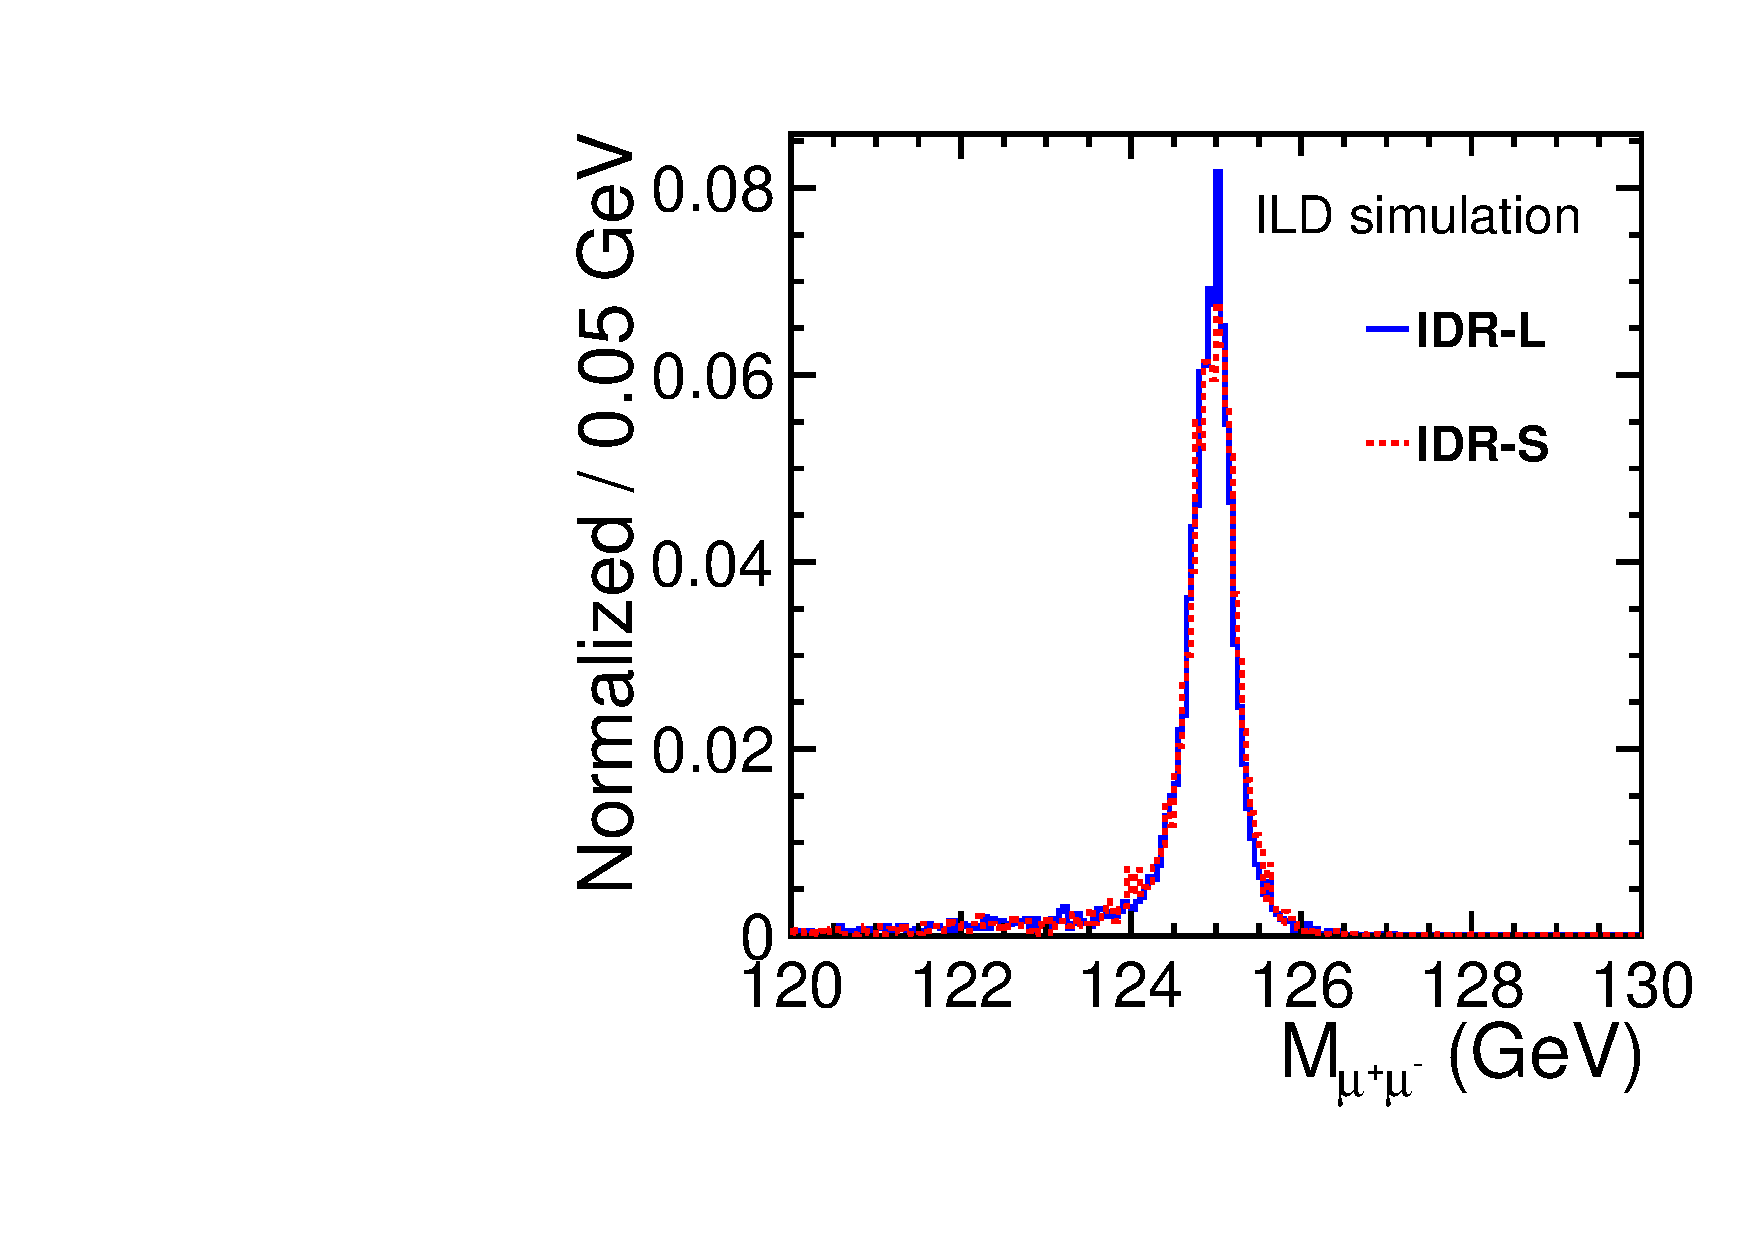
\includegraphics[width=\textwidth]{Performance/fig/mumu_mass.pdf}
\caption{ \label{fig:Hmumu:mass}}
 \end{subfigure}
%\hspace{0.03\textwidth}
\begin{subfigure}{0.49\hsize}  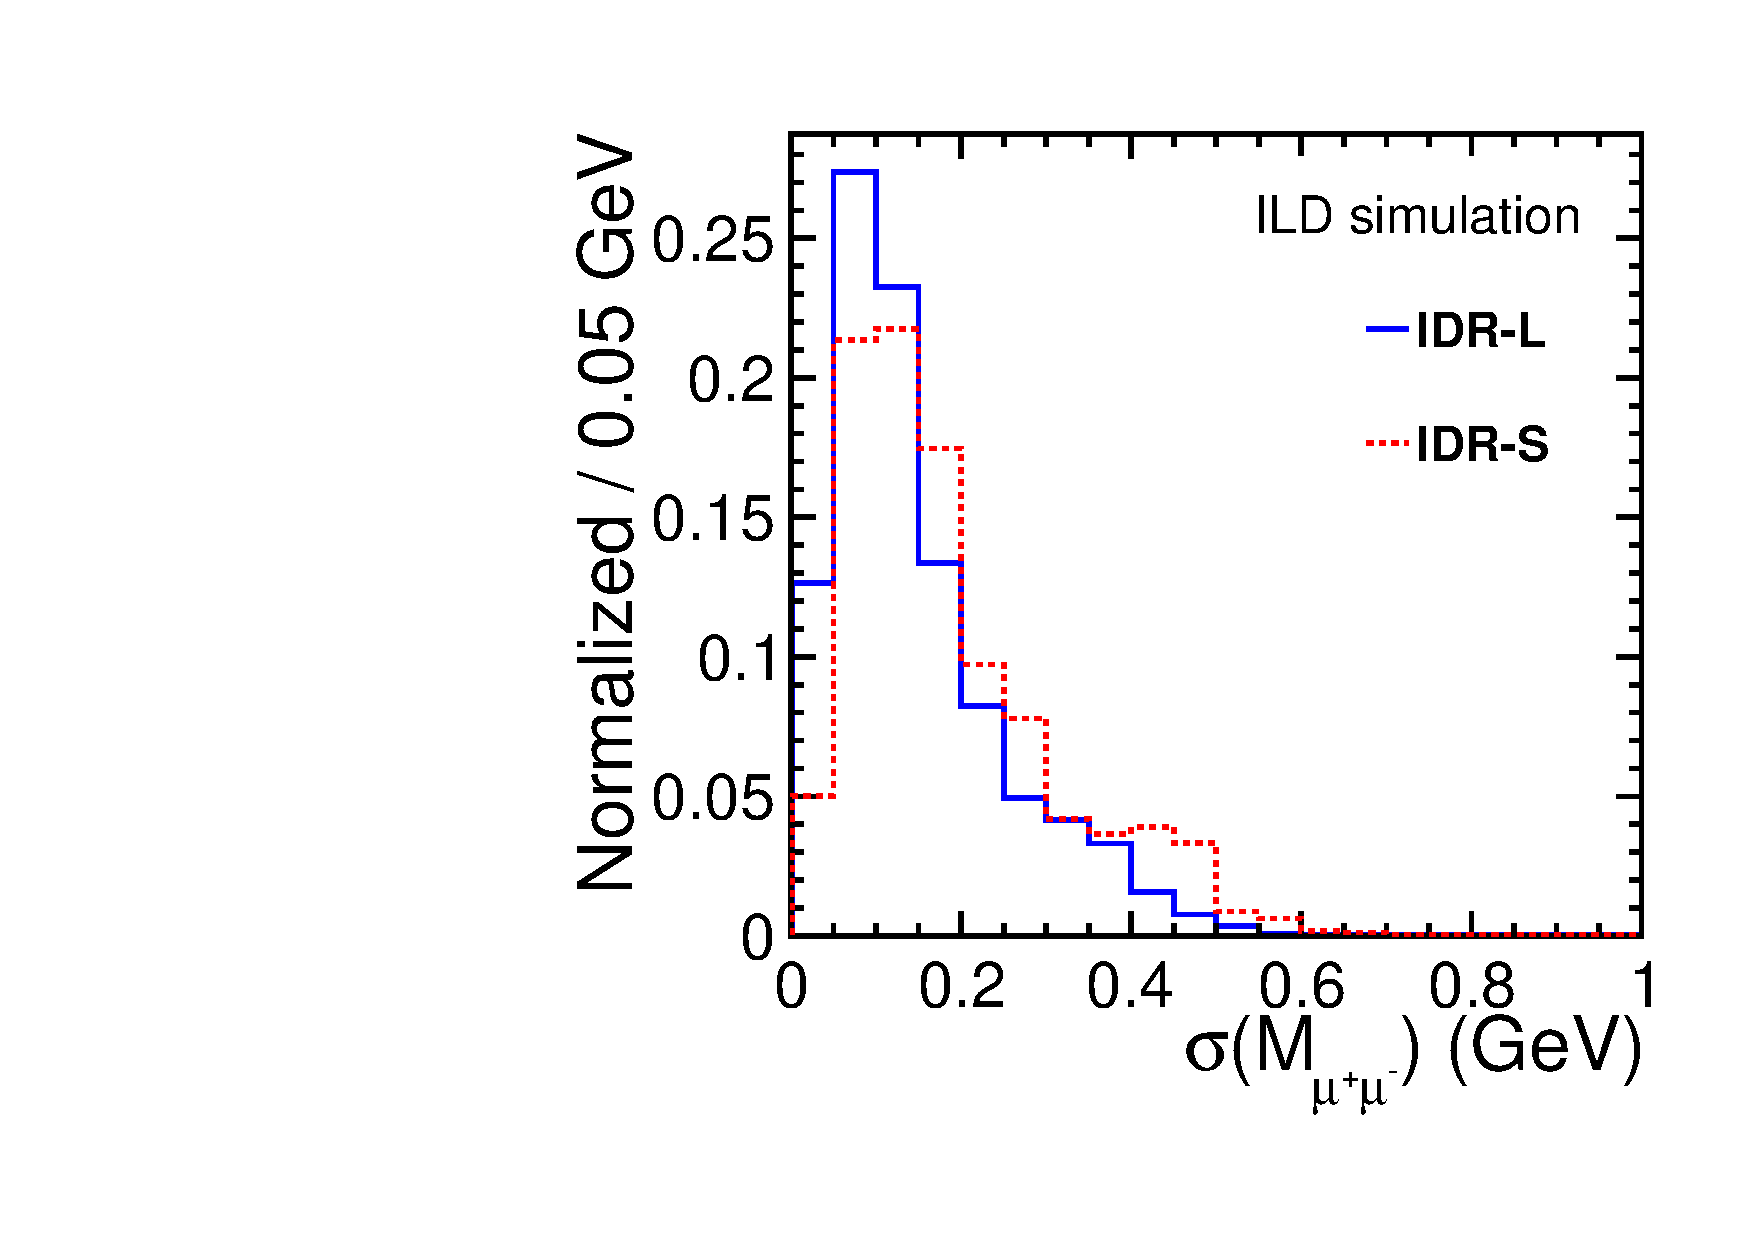
\includegraphics[width=\textwidth]{Performance/fig/sigma_mumu_mass_07.pdf}
 \caption{  \label{fig:Hmumu:sigma}}
 \end{subfigure}
%\end{center}
\caption{$\nu\bar{\nu} H \to \nu\bar{\nu} \mu^+\mu^-$ benchmark for ILC500 as defined in Sec.~\ref{sec:benchmarks:lep}:
(a) di-muon invariant mass for all selected signal events
(b) event-by-event mass uncertainty as calculated from the track covariance matrices for the case that both muons are in the barrel region of the detector ($|\cos{\theta}| < 0.7$)
}
\label{fig:Hmumu}
\end{figure}

After the event selection, about $33$ signal events, corresponding to a selection efficiency of $58\%$, remain over a evenly distributed background of about $1100$ events (counted in a mass window between $120$ and $130$\,GeV) for ILC500 as defined in Sec.~\ref{sec:benchmarks:lep}. Finally, the expectation values for the number of signal events observable above the backgrounds as well as for its uncertainty are obtained from many toy MC fits to the di-muon invariant mass spectrum~\cite{ILDNote:Hmumu}. The obtained precisions on $\sigma(\nu\bar{\nu} H)\times BR(H\to \mu^+\mu^-)$ are $40.2$\% for IDR-L and $41.3$\% for IDR-S. The relative difference of $2.8\%$ is consistent with the expectation of a $\sim 10\%$ difference in the signal peak width over a flat background. Either number, however, is about a factor $3$ worse than the asymptotic precision for the case of $100\%$ efficiency and no backgrounds, which would be 13\%. The difference is vastly dominanted by the remaining ``irreducible'' backgrounds with two muons and two neutrinos from $W$ pairs decaying either directly to muons or via tau-leptons. While there is certainly room for improvement in rejecting these backgrounds, this will factorize from the impact of the signal peak width, as long as the background remains flat in the discriminating variable. 
 


%%%%%%%%%%%%%%%%%%%%%%%%%%%%%%%%%%%%%%%%%%%%%%%%%%%%%%%%%%%%%%%%%%%
\subsection{Sensitivity to \texorpdfstring{$H \to $ invisible}{H -> invisible}}

The decay of the Higgs boson into invisible particles is of particular interest because
it could give important clues about the nature of Dark Matter. As a detector benchmark for testing the impact of the jet energy resolution, in particular the hadronic decay mode of the $Z$ boson is considered here. Thus the physics observable will be the upper limit on $\sigma(q\bar{q} H)\times BR(H \to \mbox{inv.})$.

The event selection~\cite{ILDNote:Hinv} targets events which are consistent with  a di-jet plus missing four-momentum topology, where the di-jet invariant mass should be compatible with the $Z$ boson mass. The jet finding step also serves to reject PFOs from overlay of $\gamma\gamma \to $ low-$p_t$ hadron events. The final discriminating variable is the
invariant mass of the ``invisible'' four-momentum recoiling against the $Z$ boson. 

\begin{figure}[htbp]
%\begin{center}
\begin{subfigure}{0.49\hsize} 
 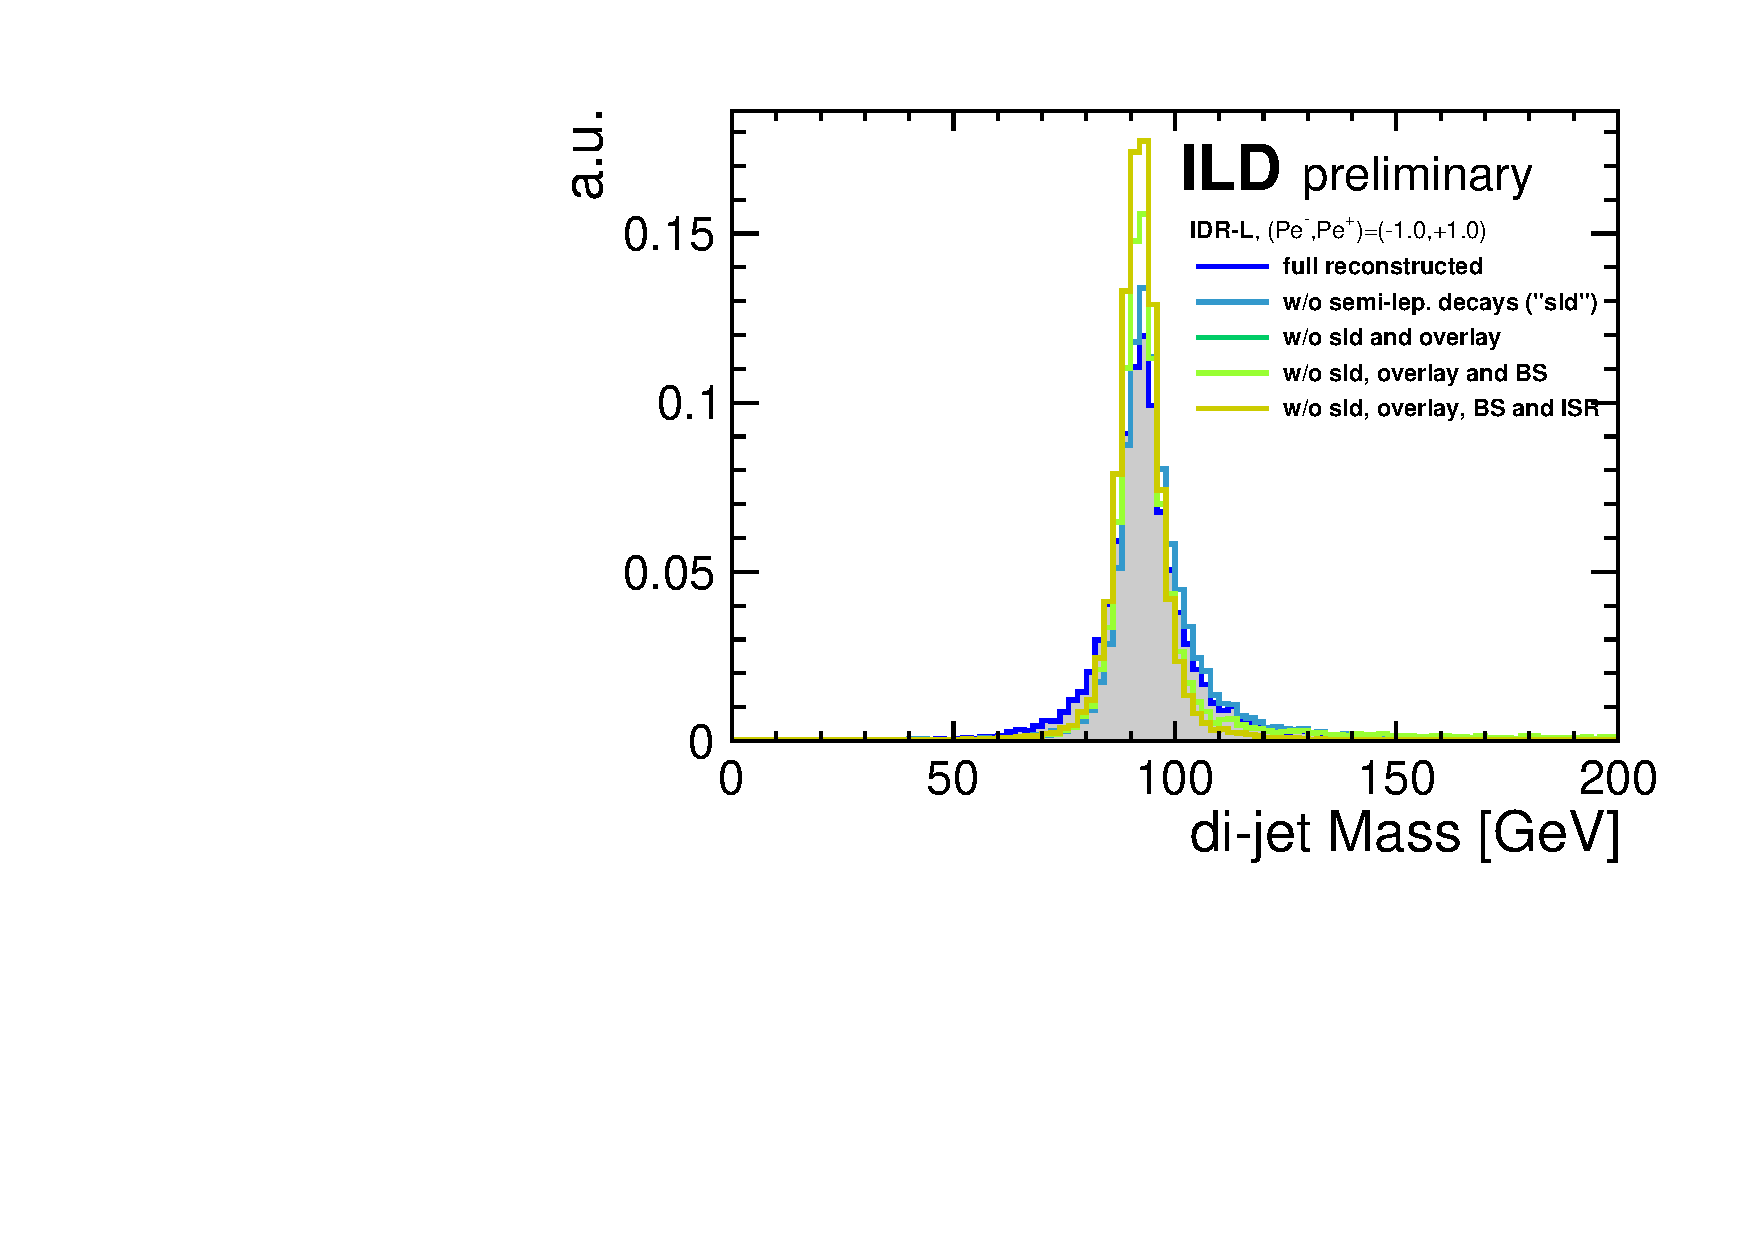
\includegraphics[width=\textwidth]{Performance/fig/compare_cheat_mjj_l5_lr.pdf}
 \caption{ \label{fig:Hinv:cheat:mjj}}
 \end{subfigure}
%\hspace{0.03\textwidth}
\begin{subfigure}{0.49\hsize} 
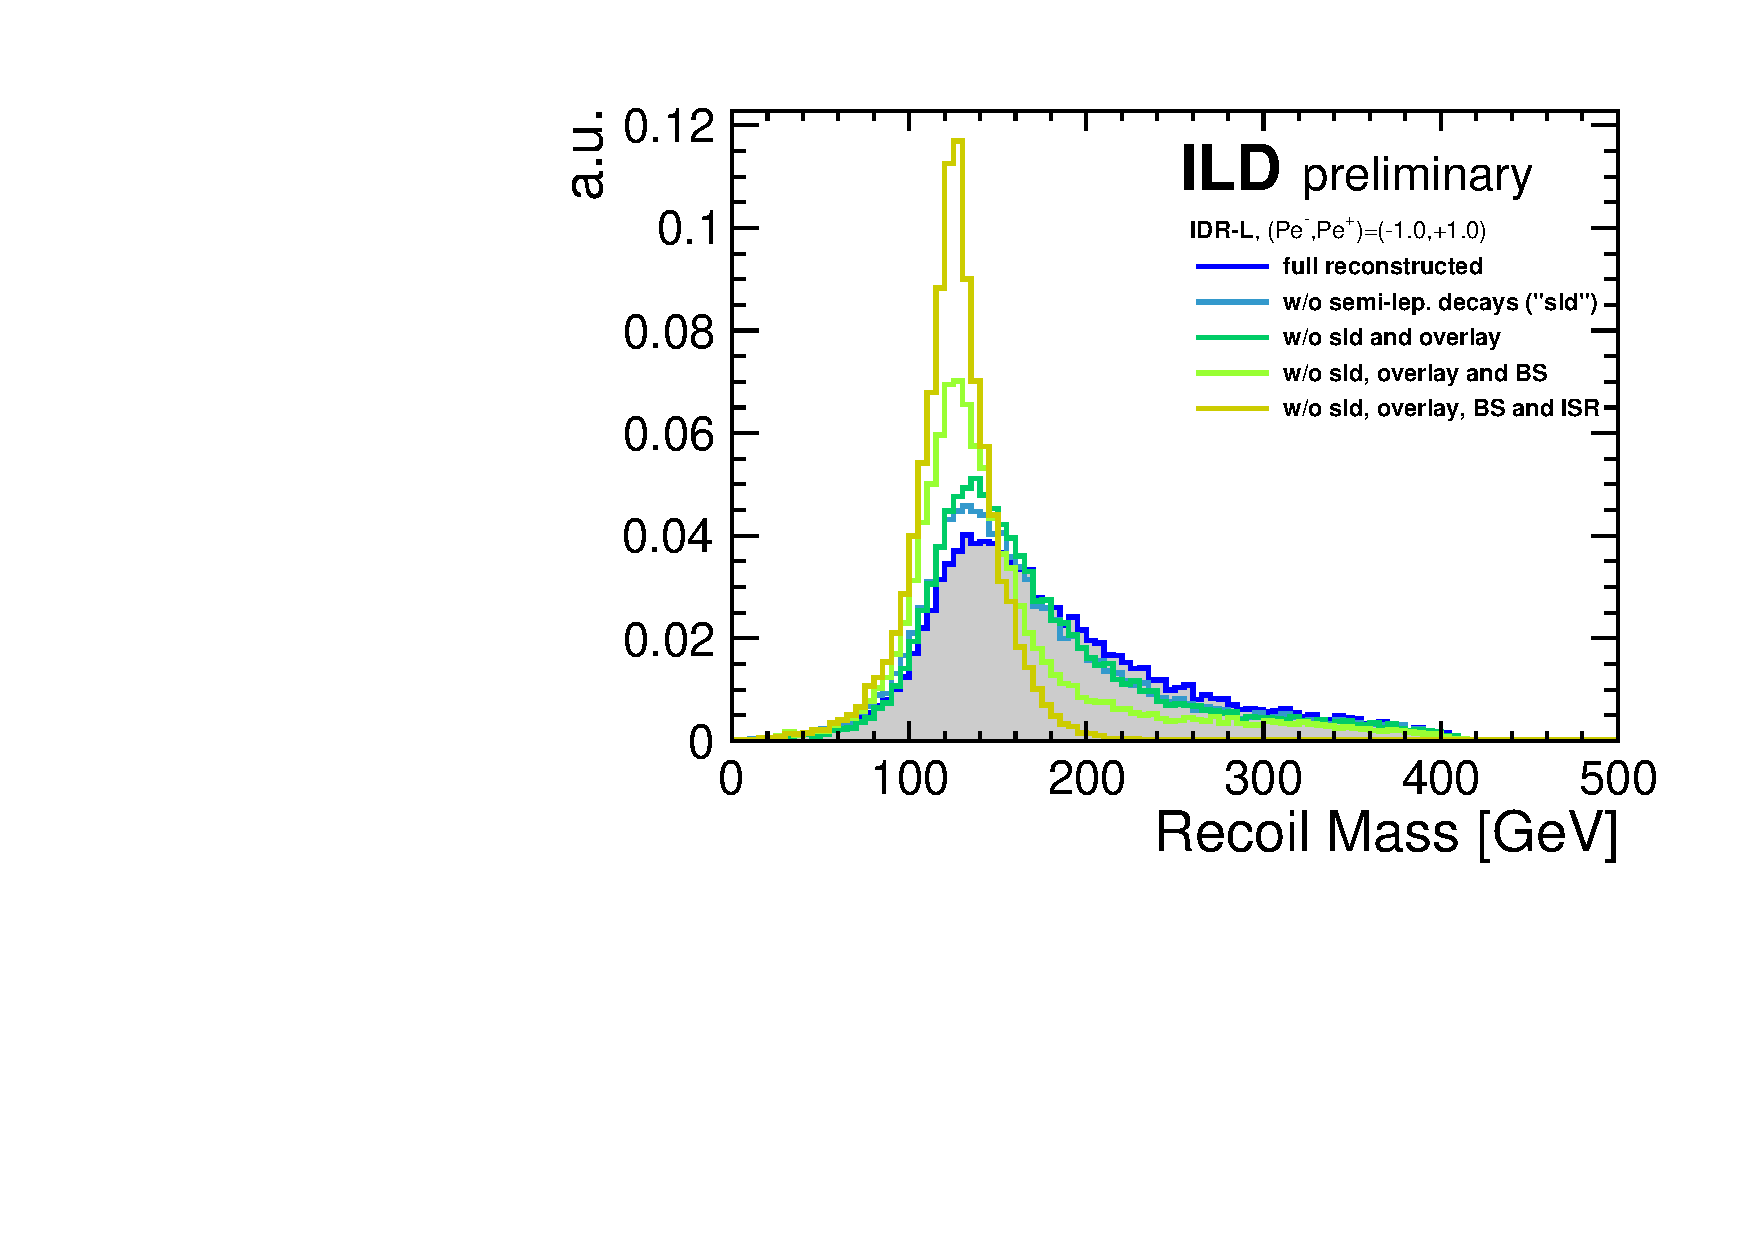
\includegraphics[width=\textwidth]{Performance/fig/compare_cheat_mrec_l5_lr.pdf}
 \caption{  \label{fig:Hinv:cheat:mrec}}
 \end{subfigure}
%\end{center}
\caption{Impact of various effects on
(a) the invariant di-jet mass and
(b) the recoil mass,
shown for the example of the large detector model.
}
\label{fig:Hinv:cheat}
\end{figure}

\begin{figure}[htbp]
%\begin{center}
\begin{subfigure}{0.49\hsize} 
 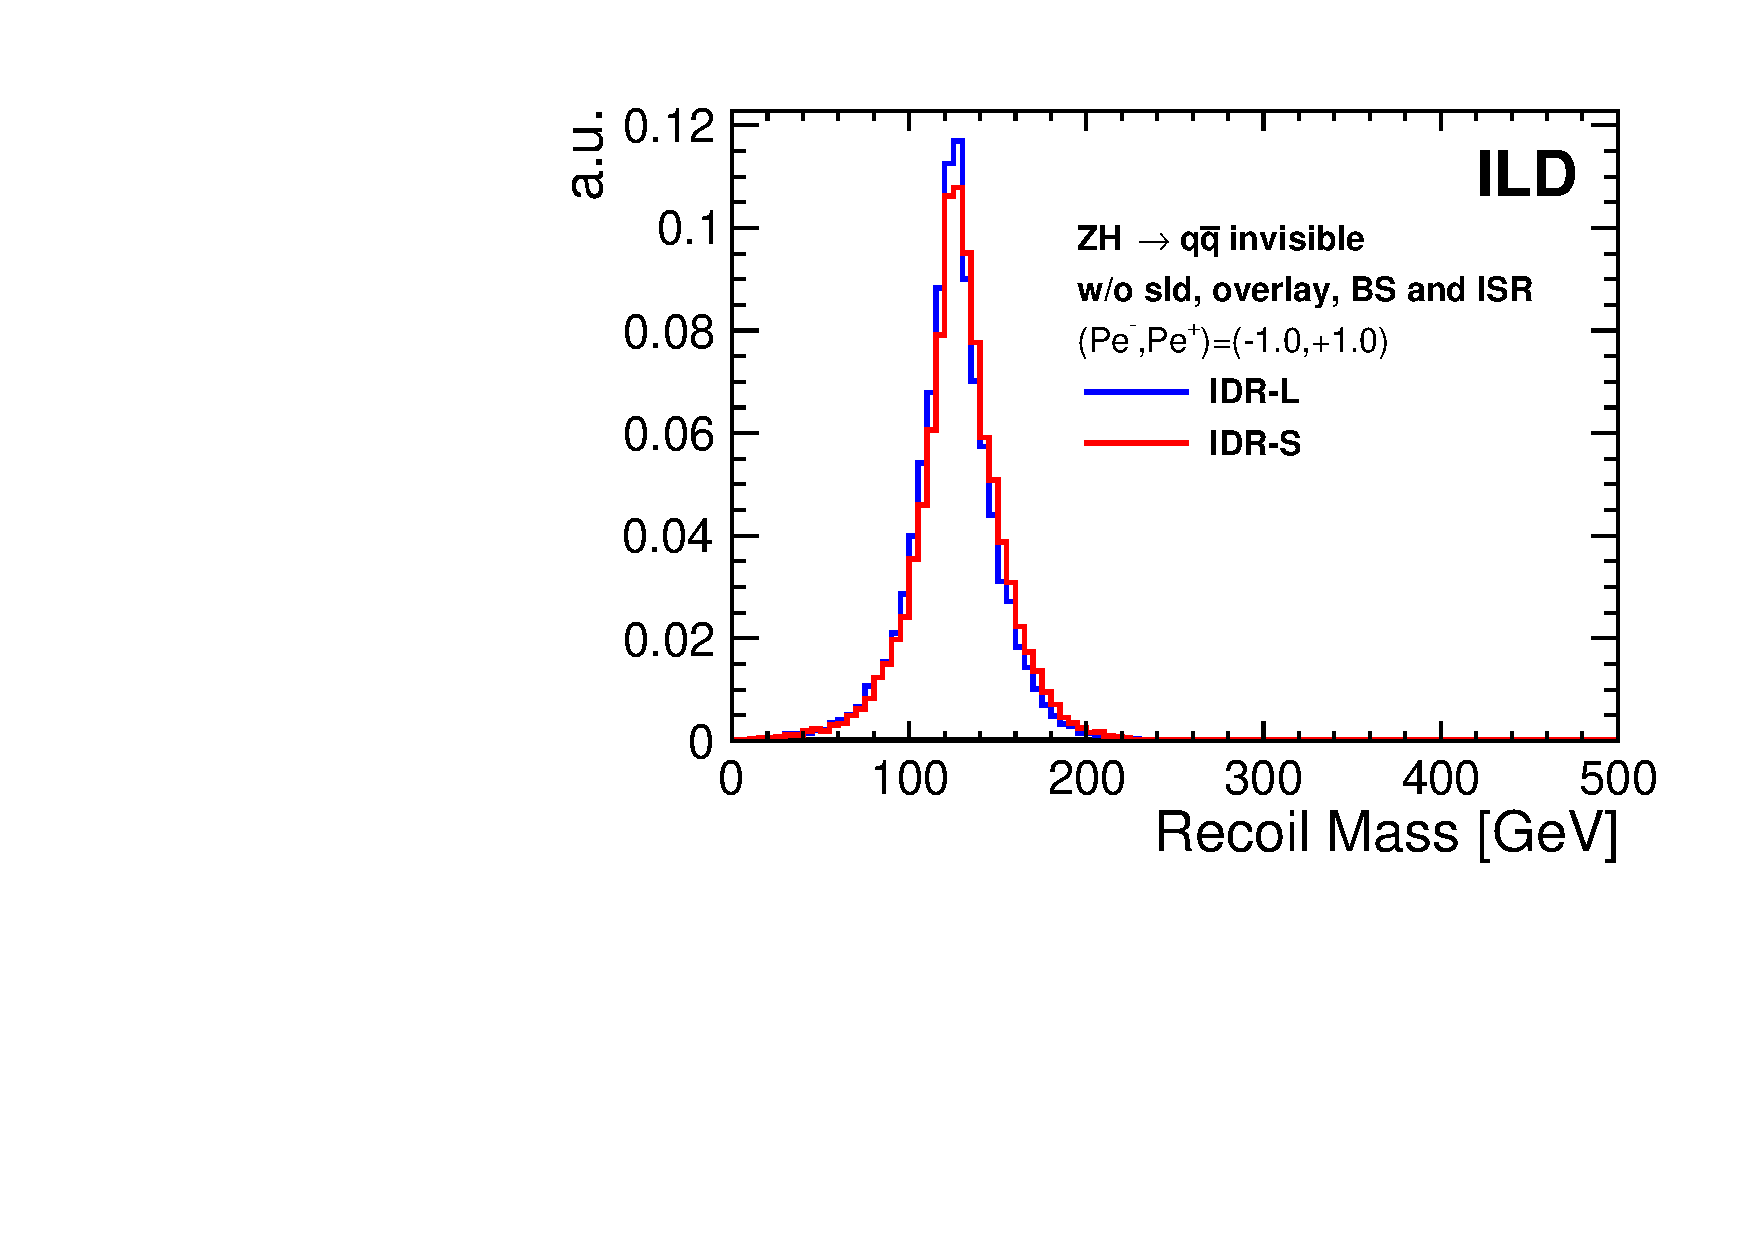
\includegraphics[width=\textwidth]{Performance/fig/compare_detector_cmrec_lr.pdf}
 \caption{ \label{fig:Hinv:comp:cheatmrec}}
 \end{subfigure}
%\hspace{0.03\textwidth}
\begin{subfigure}{0.49\hsize} 
 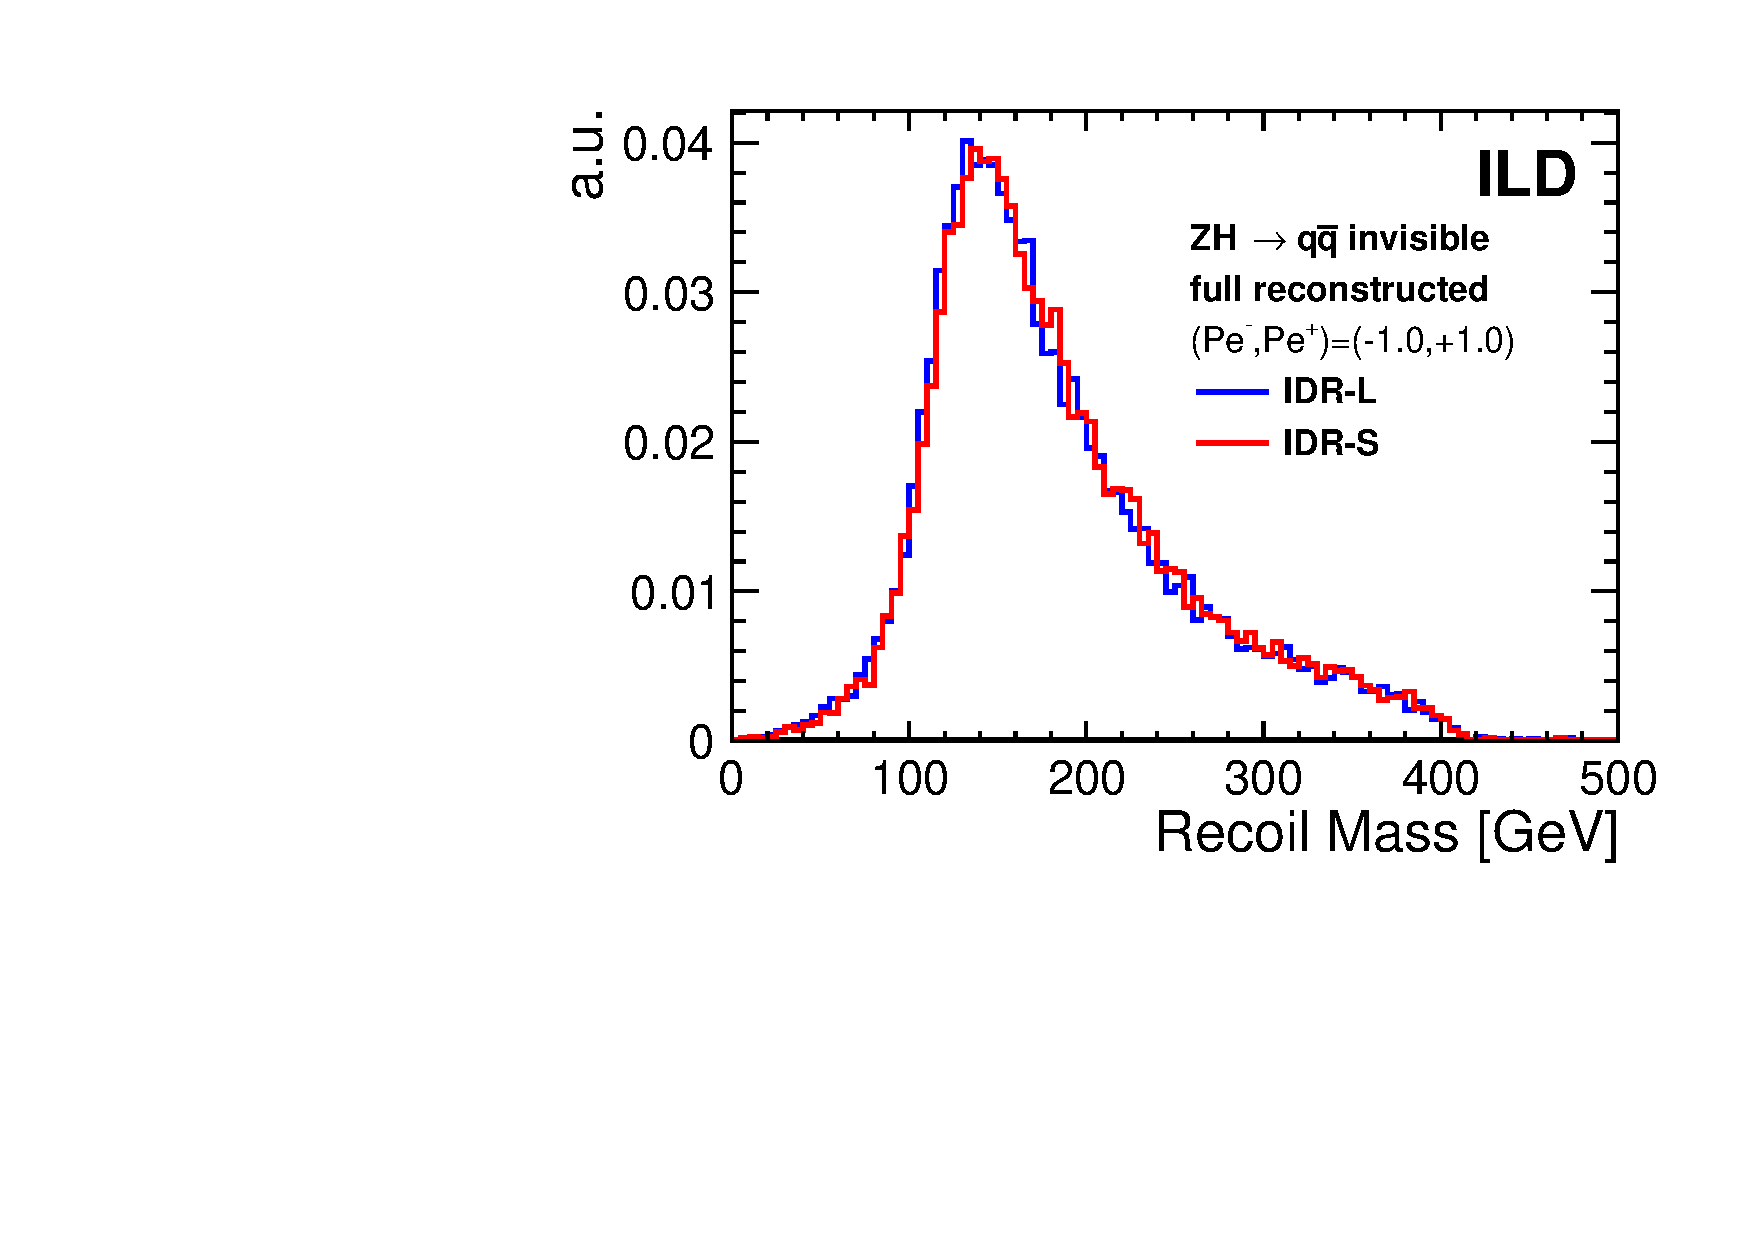
\includegraphics[width=\textwidth]{Performance/fig/compare_detector_mrec_lr.pdf}
 \caption{  \label{fig:Hinv:comp:mrec}}
 \end{subfigure}
%\end{center}
\caption{Comparison of the recoil mass distributions for IDR-L and IDR-S
(a) when cheating semi-leptonic decays, overlay removal, beam spectrum and ISR
(b) at full reconstruction level.
}
\label{fig:Hinv:comp}
\end{figure}

Figure~\ref{fig:Hinv:cheat:mjj} shows the di-jet invariant mass for the selected signal events at various levels of realism from the full reconstruction to cheating all effects apart from the detector and particle flow performance. The first step of partial cheating removes jets with semileptonic heavy flavour decays. In a detector like ILD shower shapes in the highly-granular calorimeter and specific energy loss information from the TPC should allow an
excellent identification of leptons in jets, which, combined with secondary vertex information
should allow to significantly improve scale and resolution for heavy flavour jets with semileptonic decays. However, the corresponding reconstruction algorithms are still under development and thus could not be applied here. Similarly, work is ongoing to improve the
removal of overlay backgrounds, see e.g.\ Sec.~\ref{subsec:bench:higgsino} and Ref.~\cite{Boronat:2014hva}. Thus, we expect that with future reconstruction improvements, a performance similar to the case ``w/o sld and overlay'' could be reached. The beam spectrum (BS) by construction does not affect the invariant di-jet mass. ISR, on the contrary, can lead to photons in the detector. In this analysis, no attempt has been made to identify the corresponding particle flow objects. Therefore, also a large part of the effect of ISR on the di-jet mass should be recoverable with a more sophisticated analysis. 

The corresponding situation for the recoil mass is shown in Fig.~\ref{fig:Hinv:cheat:mrec}.
Here, ISR and BS have a large impact since they lead to a deviation of the actual initial state of the hard interaction from the naive assumption. Since this effect is dominated by photons from ISR and BS which escape undetected along the beam pipe, no attempt has been made to correct the kinematics of those events in which a photon is detected. See e.g.\ Sec.~\ref{subsec:bench:extraH} for an analysis where such a correction is applied. 

The recoil mass distributions obtained with the large and small detector model are compared in Fig.~\ref{fig:Hinv:comp}. Fig.~\ref{fig:Hinv:comp:mrec} shows the situation at the current full reconstruction level, while Fig.~\ref{fig:Hinv:comp:cheatmrec} cheats the effect of semi-leptonic decays (``w/o sld''), overlay removal (``overlay''), beam spectrum (``BS'') and ISR. In both cases, the recoil  mass is slightly shifted to higher values in case of the small detector, due to differences 
in the calibration of the particle flow for the two models. In addition, the cheated recoil mass distribution is a bit wider for the small detector, by about 15\% when considering the gaussian core of the peak, as expected from its slightly worse
JER, c.f.\ Fig.~\ref{fig:perf:pfa_jer} for the barrel and Fig.~\ref{fig:perf:pfa_jer_endcap} for the endcaps.

\begin{figure}[htbp]
\begin{center}
 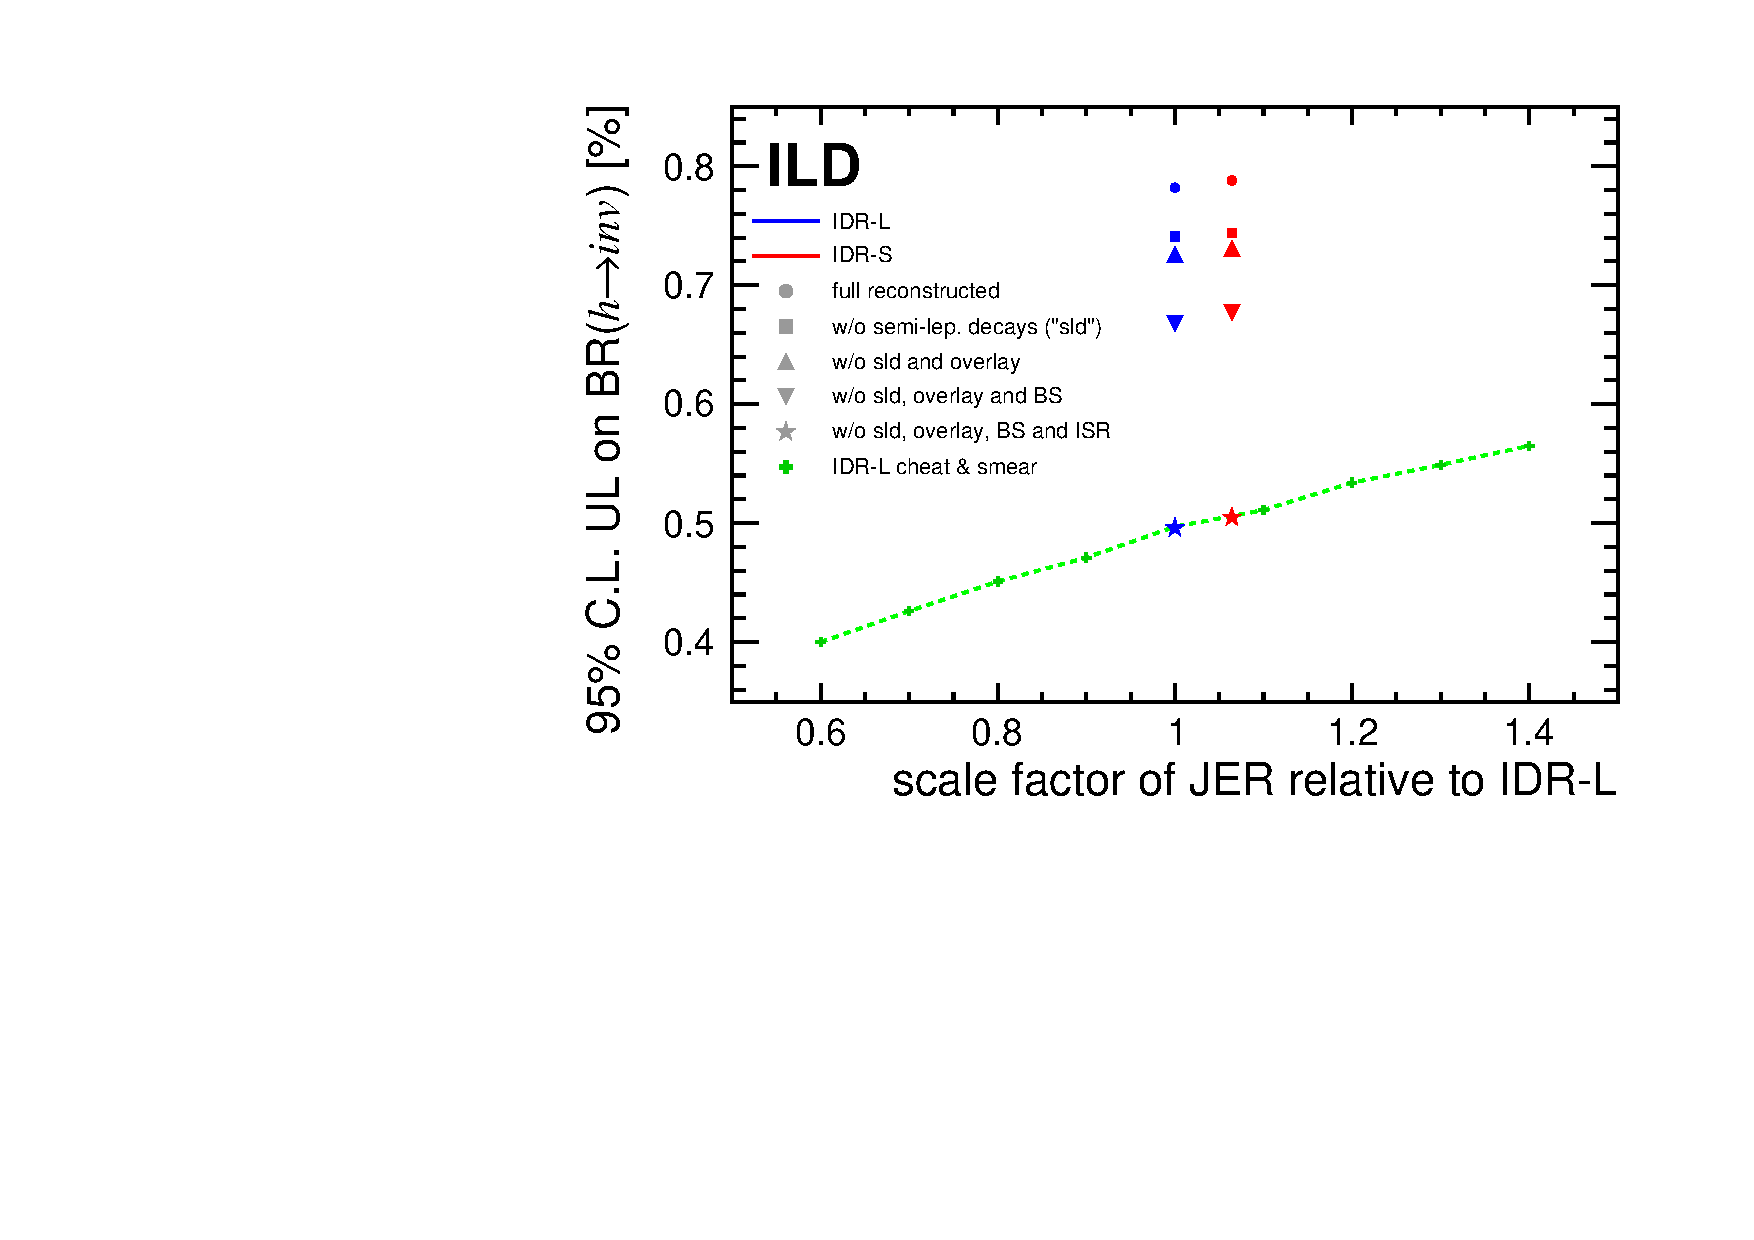
\includegraphics[width=0.75\textwidth]{Performance/fig/performance_plot.pdf}
\end{center}
\caption{Upper limit on $BR( \to $ invisible) at $95\%$ C.L. for ILC500 as defined in Sec.~\ref{sec:benchmarks:lep} as a function of the jet energy resolution. The blue and red symbols show the results obtained from simulation of the IDR-L and IDR-S detector models, respectively, in full reconstruction and at various levels of cheating. The green crosses are obtained by varying the JER up and down w.r.t.\ IDR-L.
}
\label{fig:Hinv:BRlimit}
\end{figure}

The results in terms of the physics observable, namely the $95\%$ C.L.\ upper limit on $\sigma(q\bar{q} H)\times BR(H \to \mbox{inv.})$, are summarized in Fig.~\ref{fig:Hinv:BRlimit} for both detector models at the various cheating levels. In the case of full reconstruction, the upper limit is at 0.78\%  for IDR-L  and at  0.79\%  for IDR-S, corresponding to a relative change of about 1\%. When isolating the effect of the particle flow performance by cheating all other aspects, the limit would be 0.50\% (0.51\%) for IDR-L (IDR-S), i.e.\ a relative change of about 2\%. Also displayed is an estimate of how
the cheated results would change when scaling the JER up and down. This is achieved by fitting the fully reconstructed recoil mass distribution, scaling its width and then generating toy distributions according to the scaled functions. The scale factor with respect to the IDR-L mass resolution is given on the horizontal axis. This clearly shows that
larger variations of the JER, by 20\% or so, have a clear impact on this physics analysis.
In the case of $\sqrt{s}=250$\,GeV, the impact of ISR and BS is much smaller, increasing the relative contribution from the JER.




%%%%%%%%%%%%%%%%%%%%%%%%%%%%%%%%%%%%%%%%%%%%%%%%%%%%%%%%%%%%%%%%%%%
%\subsection{\texorpdfstring{$\tau$}{Tau} decay modes and polarisation, \texorpdfstring{$A_{FB}$ and $A_{LR}$ in $e^+e^- \to \tau^+\tau^-$}{AFB and ALR in e+e- -> tau tau}}
\subsection{\texorpdfstring{$\tau$}{Tau} polarisation \texorpdfstring{in $e^+e^- \to \tau^+\tau^-$}{in e+e- -> tau tau}}

As shown in Sec.~\ref{sec:perf:hlr:tau}, the smaller ECAL inner radius of the small detector model slightly reduces the ability to identify the correct number of photons in
highly-boosted $\tau$ decays. Using the product of efficiency times purity as a figure of merit, this leads to a $5\%$ worse identification of $\tau \to \pi \nu$ and $\tau \to \rho \nu$ decays, while the identification of $\tau \to a_1 \nu$ decays deteriorates by about $15\%$ relative, c.f.\ Fig.~\ref{fig:HLR-tauID}. 

In order to evaluate the impact of this difference in a physics example, the measurement of the $\tau$ polarisation in $e^+e^- \to \tau^+\tau^-$ has been studied, looking specifically at events with no significant ISR, so those {\em not} returning to the $Z$ pole. For the $\tau \to \pi \nu$ channels, the magnitude of the $\pi^{\pm}$ momentum can directly be used to extract the polarisation. In case of the $\tau \to \rho \nu$ decay, a polarimeter vector is constructed from the momenta of the $\pi^{\pm}$ and the $\pi^0$. A detailed description of the analysis and the polarisation extraction can be found in~\cite{ILDNote:tautau}.

\begin{figure}[htbp]
\begin{center}
 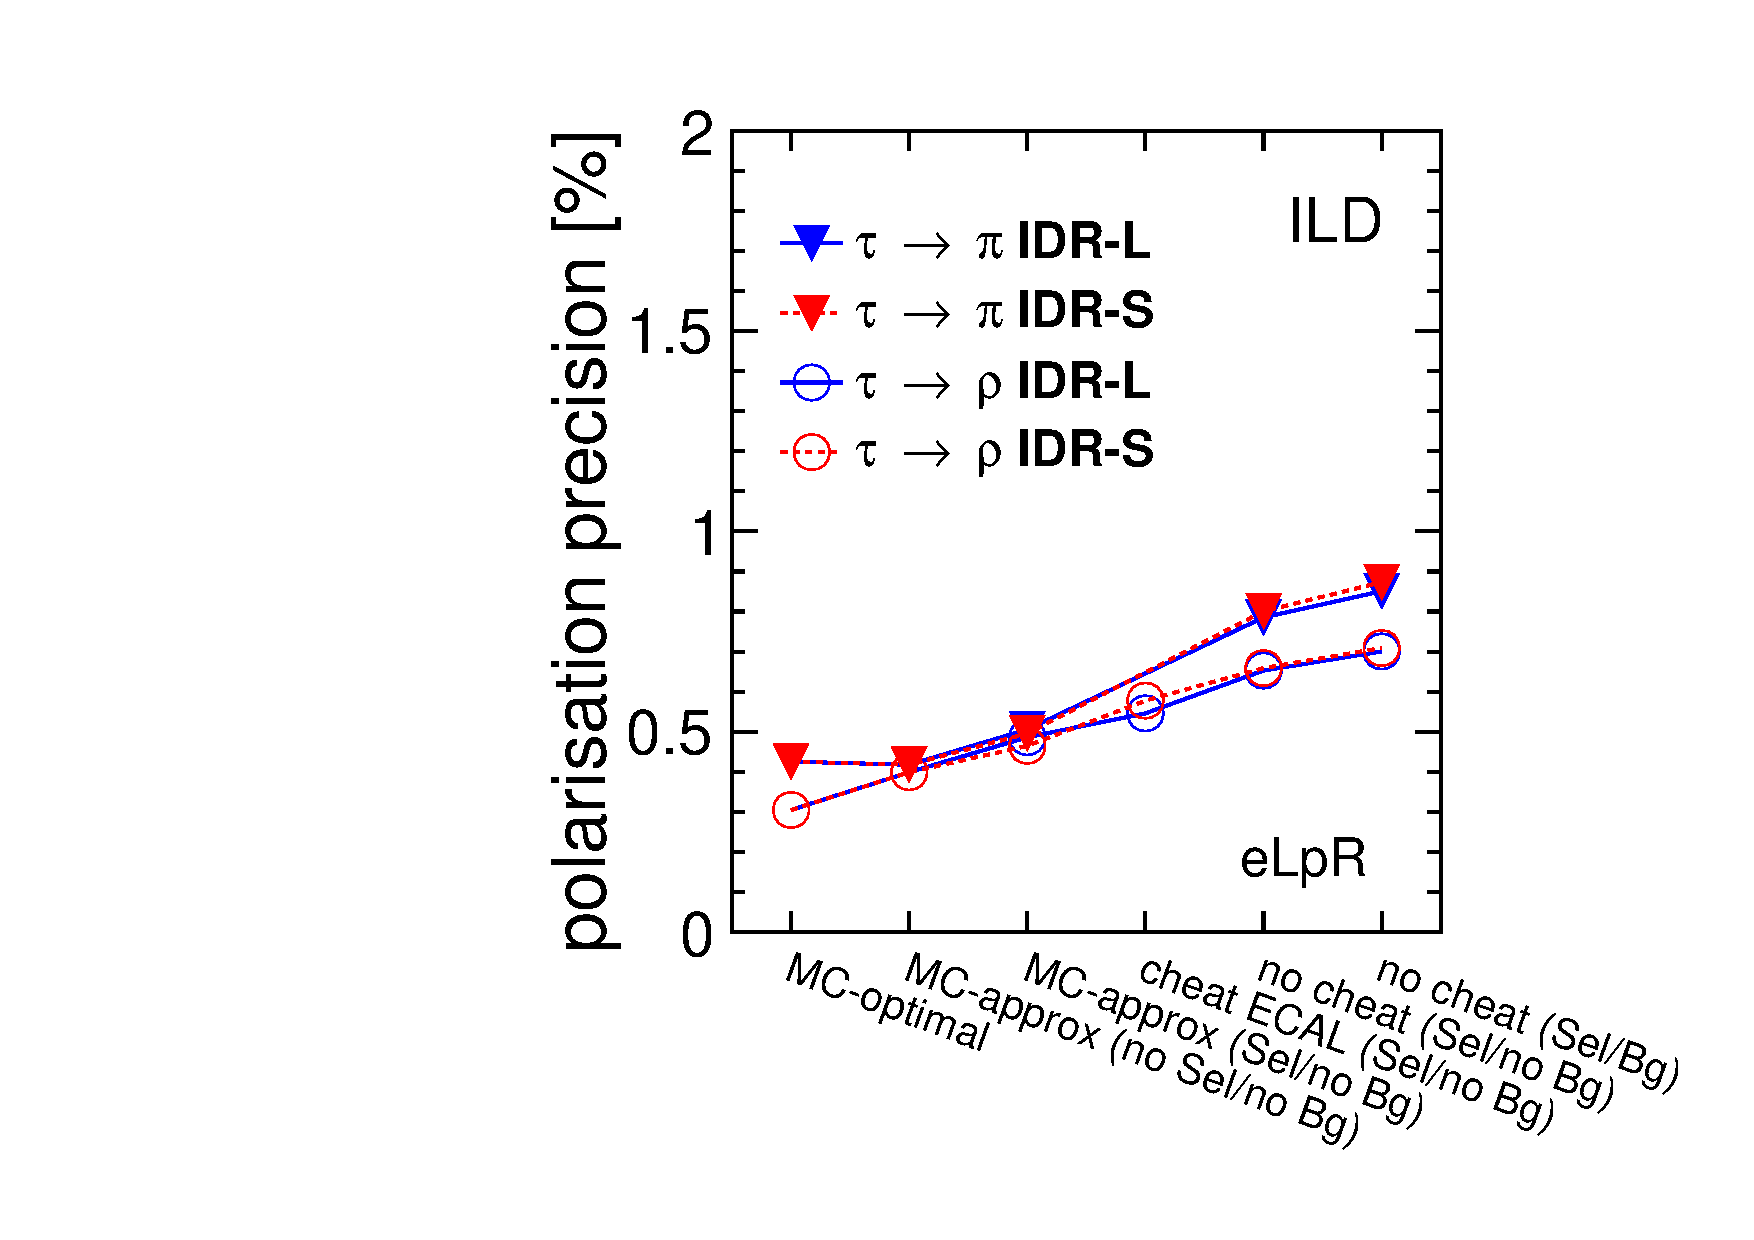
\includegraphics[width=0.55\textwidth]{Performance/fig/drawpexpresults0.pdf}
\end{center}
\caption{Precision on the $\tau$ polarisation achieved with IDR-L and IDR-S at various levels of cheating (see text) based on the $\pi$ and $\rho$ channels in the $P(e^-,e^+)=(-80\%,+30\%)$ data set of ILC500 as defined in Sec.~\ref{sec:benchmarks:lep}.}
\label{fig:tautau:taupol}
\end{figure}

Figure~\ref{fig:tautau:taupol} illustrates the precision on the $\tau$ polarisation achieved with IDR-L and IDR-S  based on the $\pi$ and $\rho$ channels in the $P(e^-,e^+)=(-80\%,+30\%)$ data set, which dominates the combined precision. Various
levels of cheating are shown, starting from the optimal result when using all MC information, including the neutrino momentum. The next entry shows by how much the performance in the $\rho$ channel degrades by the approximate definition of the polarimeters used here\footnote{In principle, improved methods can be used, which however need further investigation~\cite{ILDNote:tautau}.}, followed by the application of the selection efficiency. The last three steps use the fully simulated and reconstructed events, apart from the entry ``cheat ECAL'', which uses MC information for the $\pi^0$ in the $\rho$ channel. In the last step, the full SM background is added. For the $\pi$-channel, the most significant effect occurs when reducing the number of signal events according to the selection efficiency of about $55\%$ observed in the full analysis. In case of the $\rho$-channel, all steps contribute at a similar level to the final result. Overall, the differences between IDR-L and IDR-S are very small. %,  and probably due to limited MC statistics. 
%The largest deterioration of the precision occurs when applying the selection efficiency. Thus, future improvements of the di-$\tau$ selection have the largest potential for improving this measurement.

% \begin{figure}[htbp]
% %\begin{center}
% \begin{subfigure}{0.49\hsize} 
% %\includegraphics[width=\textwidth]{Performance/fig/}
%  \caption{ \label{fig:}}
%  \end{subfigure}
% %\hspace{0.03\textwidth}
% \begin{subfigure}{0.49\hsize} 
% %\includegraphics[width=\textwidth]{Performance/fig/}
%  \caption{  \label{fig:}}
%  \end{subfigure}
% %\end{center}
% \caption{
% (a) 
% (b) 
% }
% \label{fig:}
% \end{figure}

%%%%%%%%%%%%%%%%%%%%%%%%%%%%%%%%%%%%%%%%%%%%%%%%%%%%%%%%%%%%%%%%%%%
%\subsection{\texorpdfstring{$W$}{W} mass, Triple Gauge Couplings and Beam Polarisation from \texorpdfstring{$e^+e^- \to WW \to qql\nu$}{e+e- -> WW -> qqln}}
%%%%%%%%%%%%%%%%%%%%%%%%%%%%%%%%%%%%%%%%%%%%%%%%%%%%%%%%%%%%%%%%%%%
\subsection{Hadronic \texorpdfstring{$WW$ and $ZZ$}{WW and ZZ} separation in Vector Boson Scattering} 

Vector boson scattering is an important process for testing the unitarisation of $WW$ scattering by the Higgs boson, as well as for measuring quartic gauge couplings, and thereby probing for anomalous contributions. Among all relevant final states, the reaction $e^+e^- \to \nu\nu VV \to \nu\nu qqqq$, where $VV$ can be $WW$ or $ZZ$, poses a particular challenge to the detectors and reconstruction algorithms, since it requires the separation of the hadronic $W$ and $Z$ decays without the ability to exploit kinematic constraints, e.g.\ on the
total event energy, due to the two invisible neutrinos.

This benchmark, at a center-of-mass energy of 1\,TeV, has already been studied in full detector simulation for the ILD LoI~\cite{ild:bib:ILDloi}. All relevant aspects, in particular the full overlay from $\gamma\gamma \to$ low-$p_t$ hadrons and from $e^+e^-$ pair background, are now included for the first time, and all quark flavours are considered in the final state~\cite{ILDNote:QGCs}. Figure~\ref{fig:qgc:truejet} illustrates the ranges of jet energies and polar angles probed by this benchmark, both inclusively and for the case of high di-boson invariant
masses, which is the phase space most sensitive to new physics effects. 

\begin{figure}[htbp]
%\begin{center}
\begin{subfigure}{0.49\textwidth} 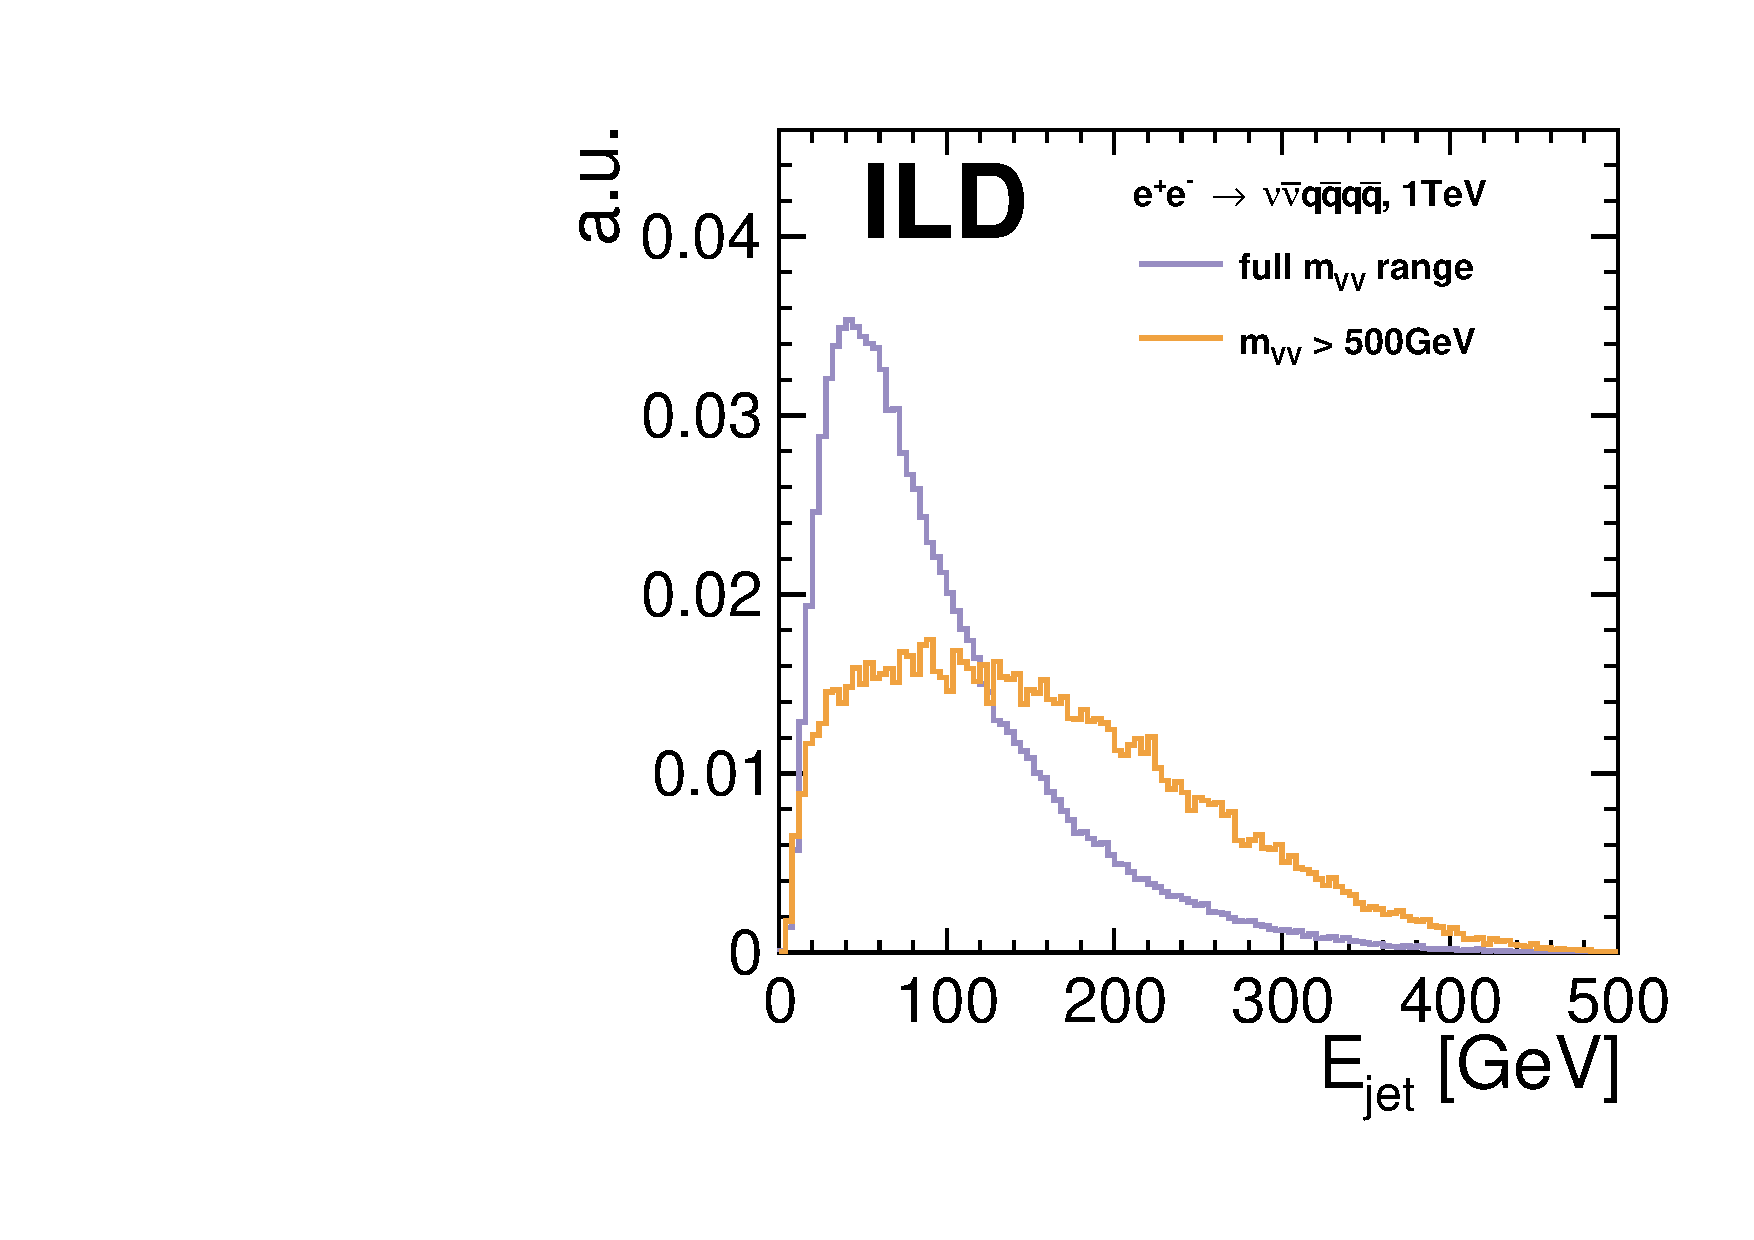
\includegraphics[width=\textwidth]{Performance/fig/comp_jet_E.pdf}
 \caption{ \label{fig:qgc:truejet:E}}
 \end{subfigure}
%\hspace{0.03\textwidth}
\begin{subfigure}{0.49\textwidth} 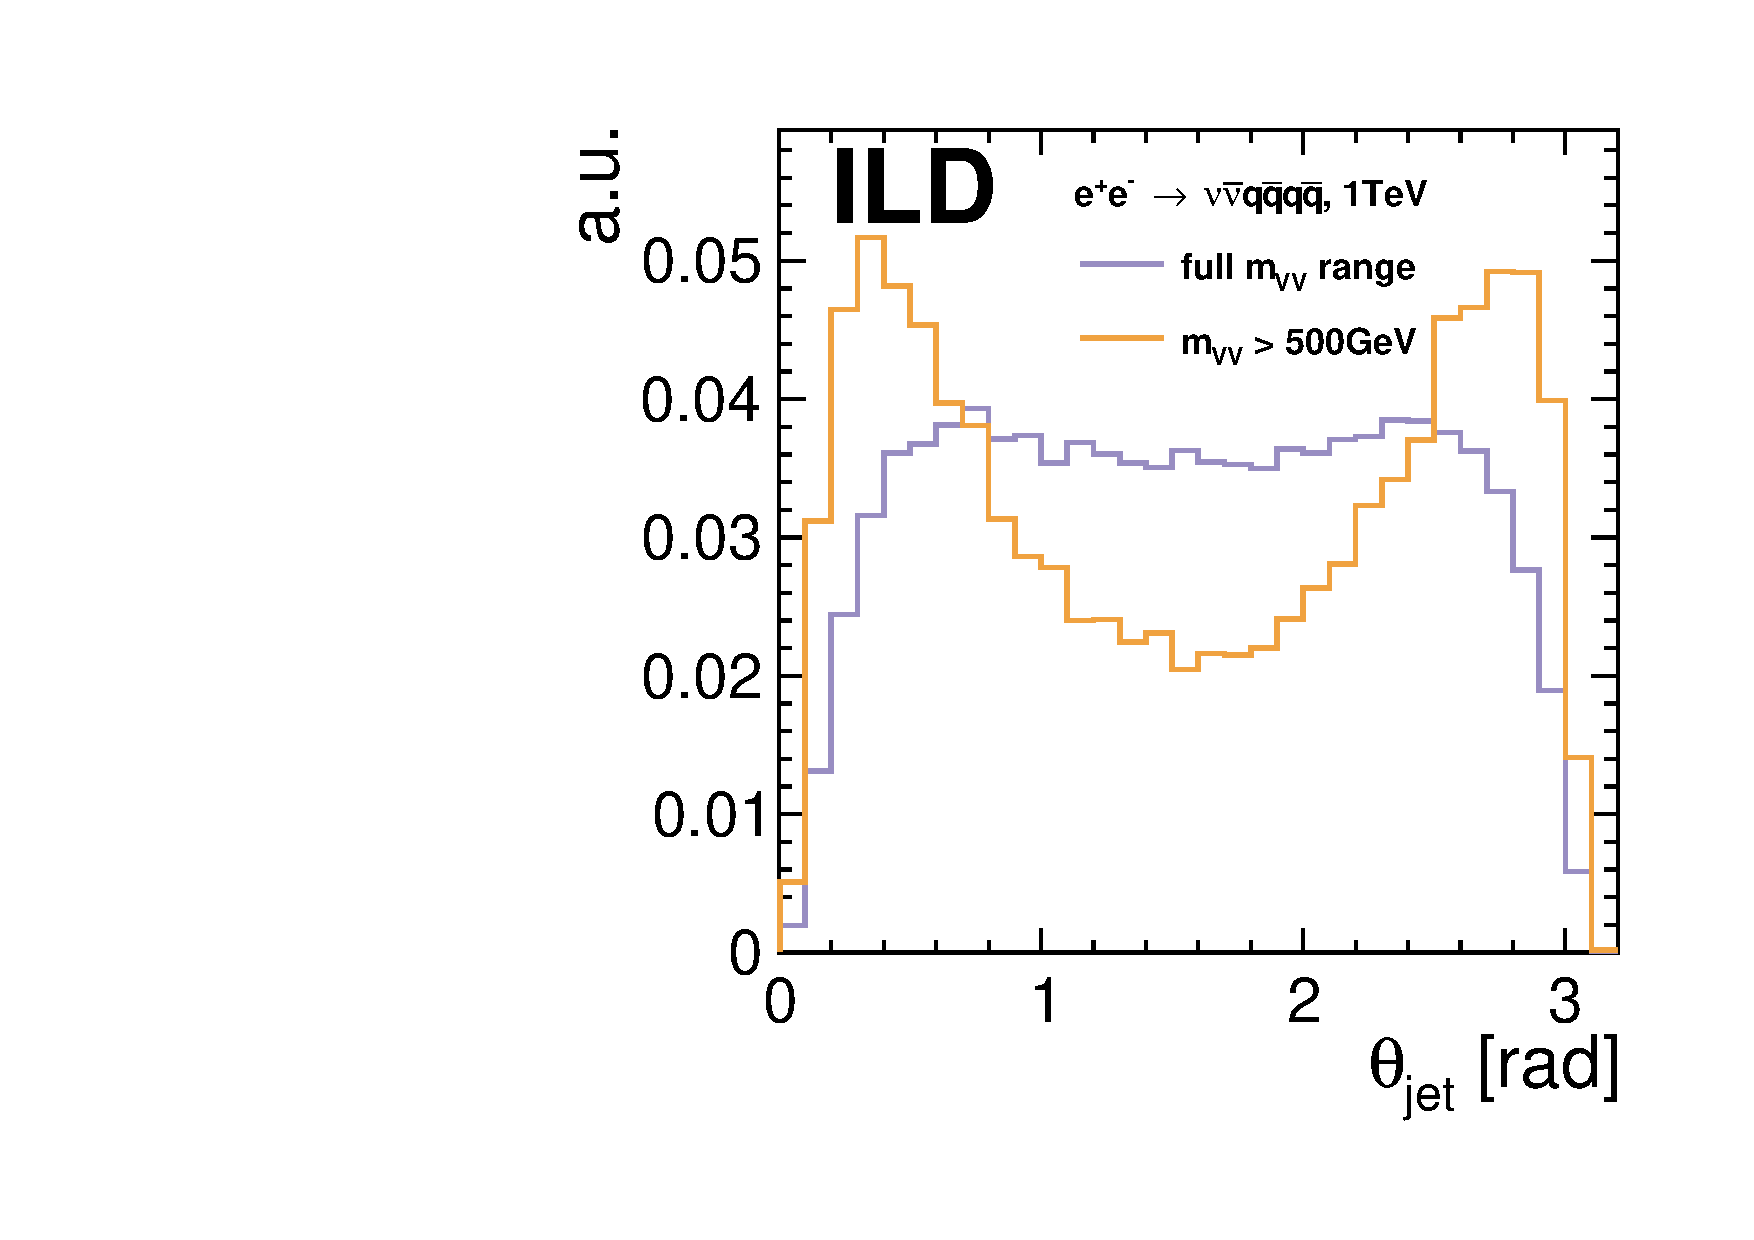
\includegraphics[width=\textwidth]{Performance/fig/comp_jet_theta.pdf}
 \caption{  \label{fig:qgc:truejet:theta}}
 \end{subfigure}
%\end{center}
\caption{(a) Energy and (b) polar angle distributions of the jets from $e^+e^- \to \nu\nu qqqq$ at $\sqrt{s}=1$\,TeV on truth level.
}
\label{fig:qgc:truejet}
\end{figure}

Jet clustering is performed in a two-step procedure, first by requesting $4$ jets with a cone radius of $1.3$ from an exclusive $k_t$ algorithm in order to remove PFOs from the overlay backgrounds. In the second step, all PFOs in the four jets are reclustered into $4$ jets with the (inclusive) $ee$ $k_t$ algorithm. The jets are paired into two boson candidates by minimizing the mass difference between the two bosons. The resulting $W$ and $Z$ mass distributions
are shown in Fig.~\ref{fig:qgc:rec}. Fig.~\ref{fig:qgc:rec:1d} shows the average di-jet mass per event, comparing ILD-L and ILD-S, while Fig.~\ref{fig:qgc:rec:2d} shows the 2-dimensional distribution in the mass plane of the two invariant di-jet masses for ILD-L. At this level, no significant difference between the detector models can be observed.


%\thisfloatsetup{floatwidth=\SfigwFull,capposition=below}
\begin{figure}[htbp]
%\begin{center}
\begin{subfigure}{0.455\hsize} 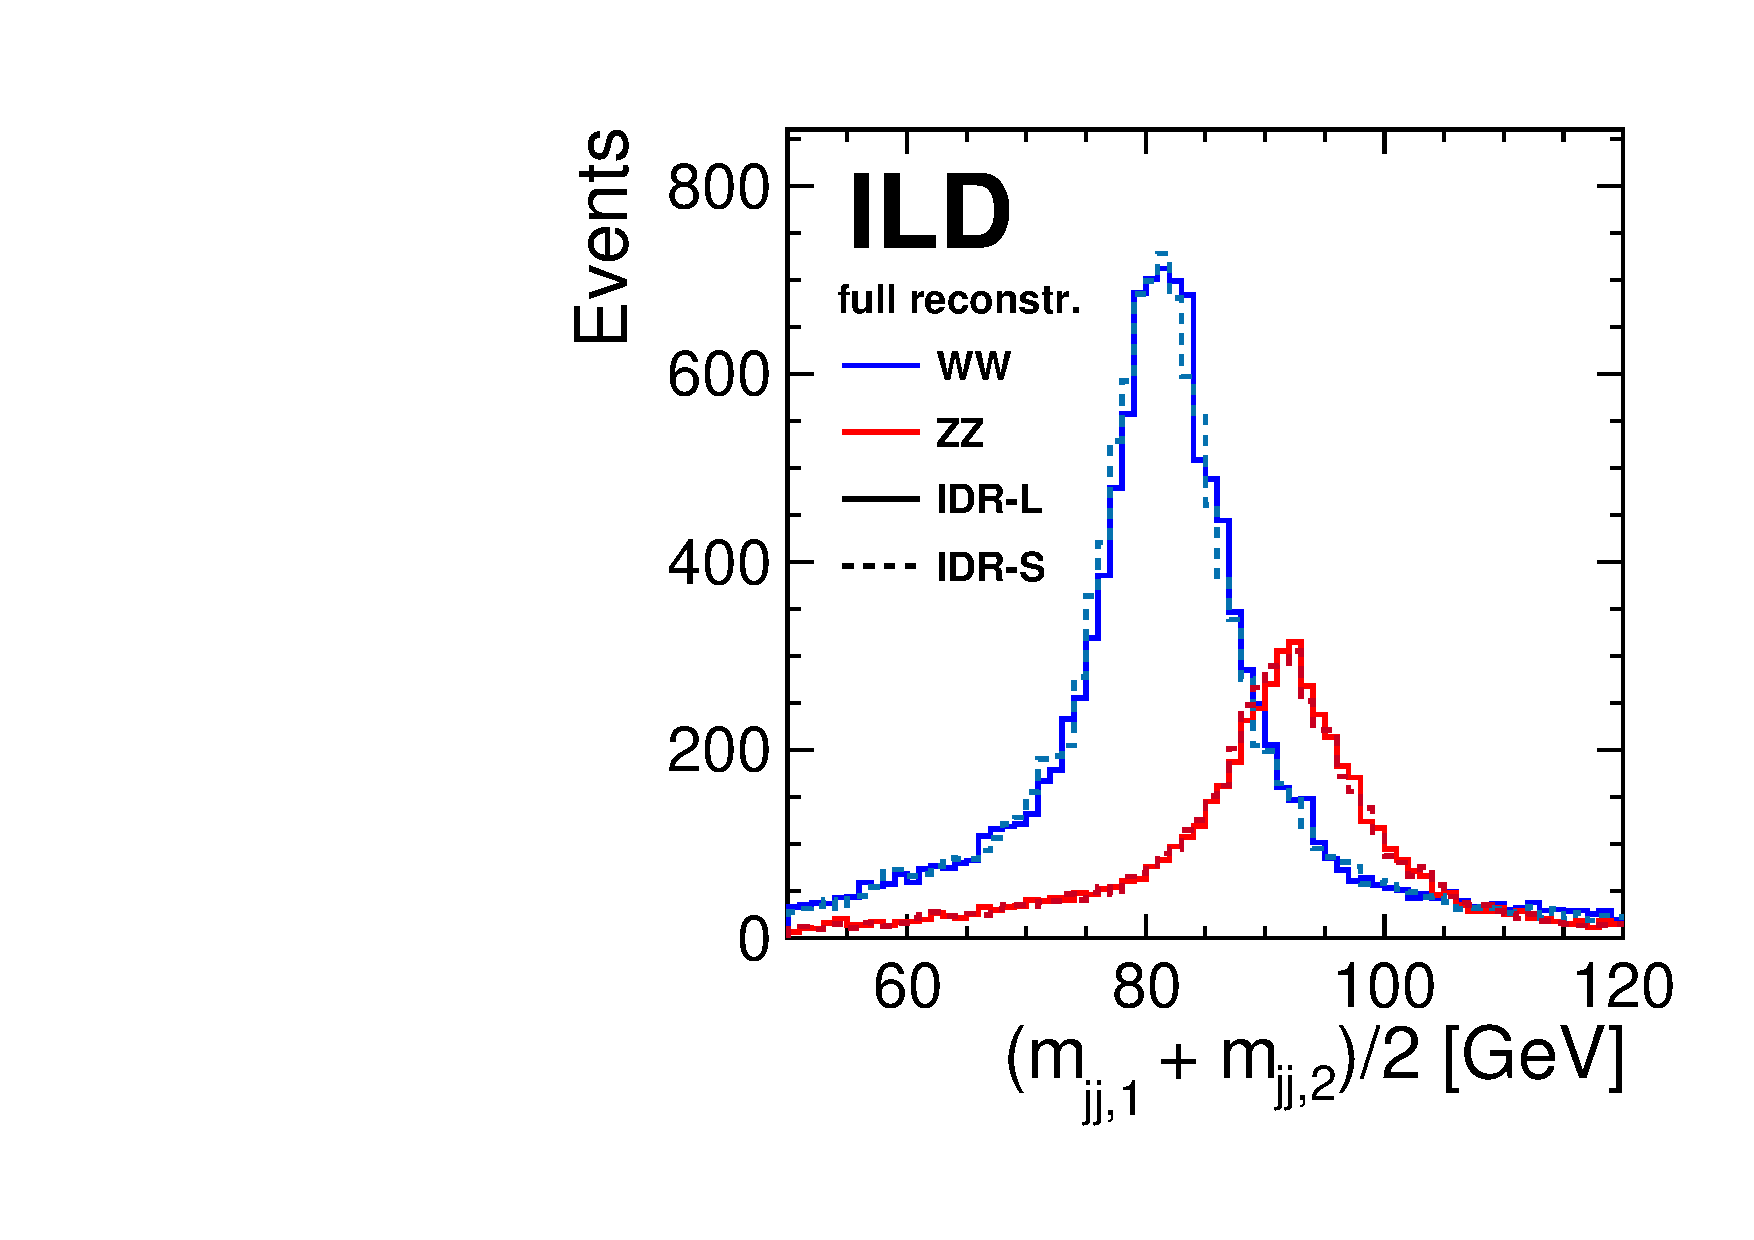
\includegraphics[width=\textwidth]{Performance/fig/ls_comp_rec_monly.pdf}
 \caption{ \label{fig:qgc:rec:1d}}
 \end{subfigure}
%\hspace{0.03\textwidth}
\begin{subfigure}{0.49\hsize} 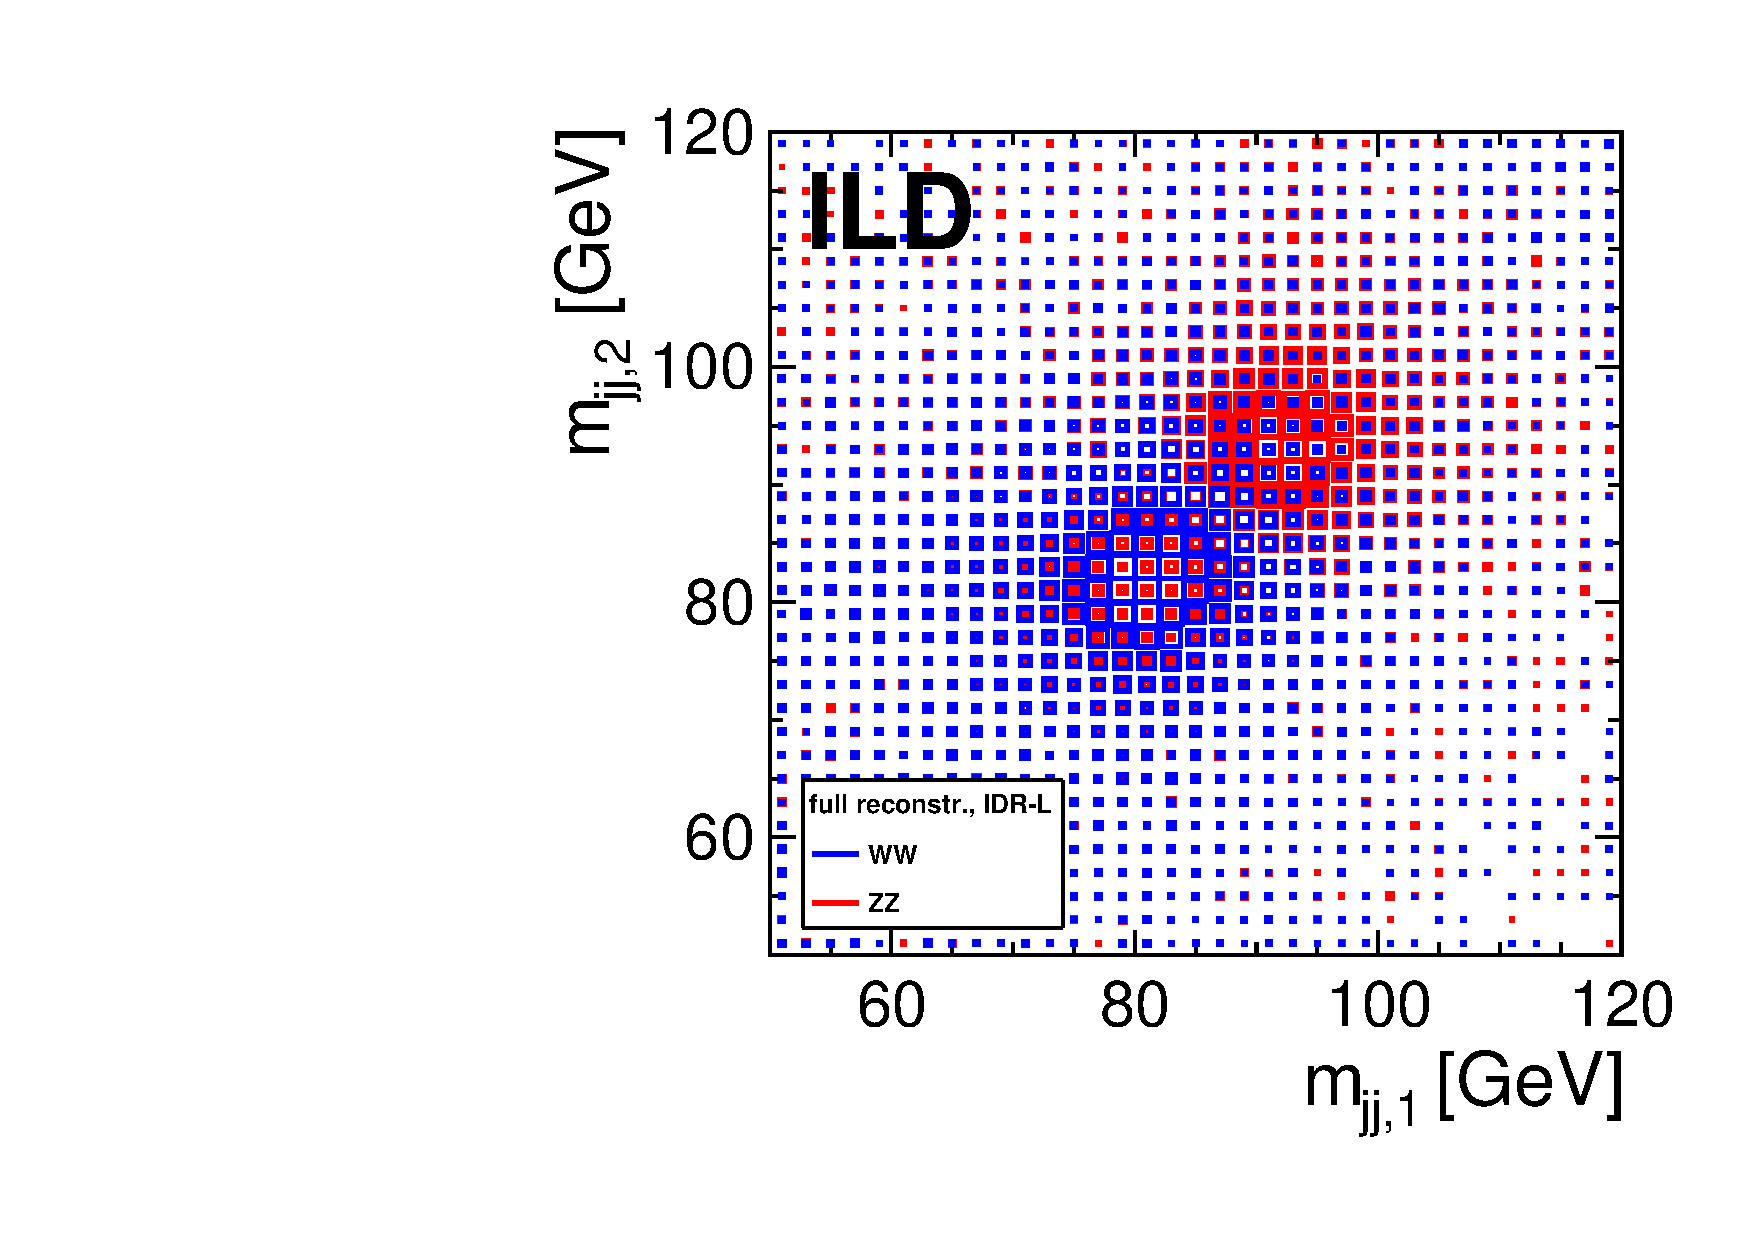
\includegraphics[width=\textwidth]{Performance/fig/m_m_rec.pdf}
 \caption{  \label{fig:qgc:rec:2d}}
 \end{subfigure}
%\end{center}
\caption{Dijet masses in $e^+e^- \to \nu\nu WW$ (blue) and $e^+e^- \to \nu\nu ZZ$ (red) events as obtained from the current full reconstruction for ILC1000 as defined in Sec.~\ref{sec:benchmarks:lep}.
(a) Average of the two di-jet masses per event.
(b) 2D illustration of the two di-jet masses per event. 
}
\label{fig:qgc:rec}
\end{figure}


\begin{figure}[htbp]
%\begin{center}
\begin{subfigure}{0.475\hsize} 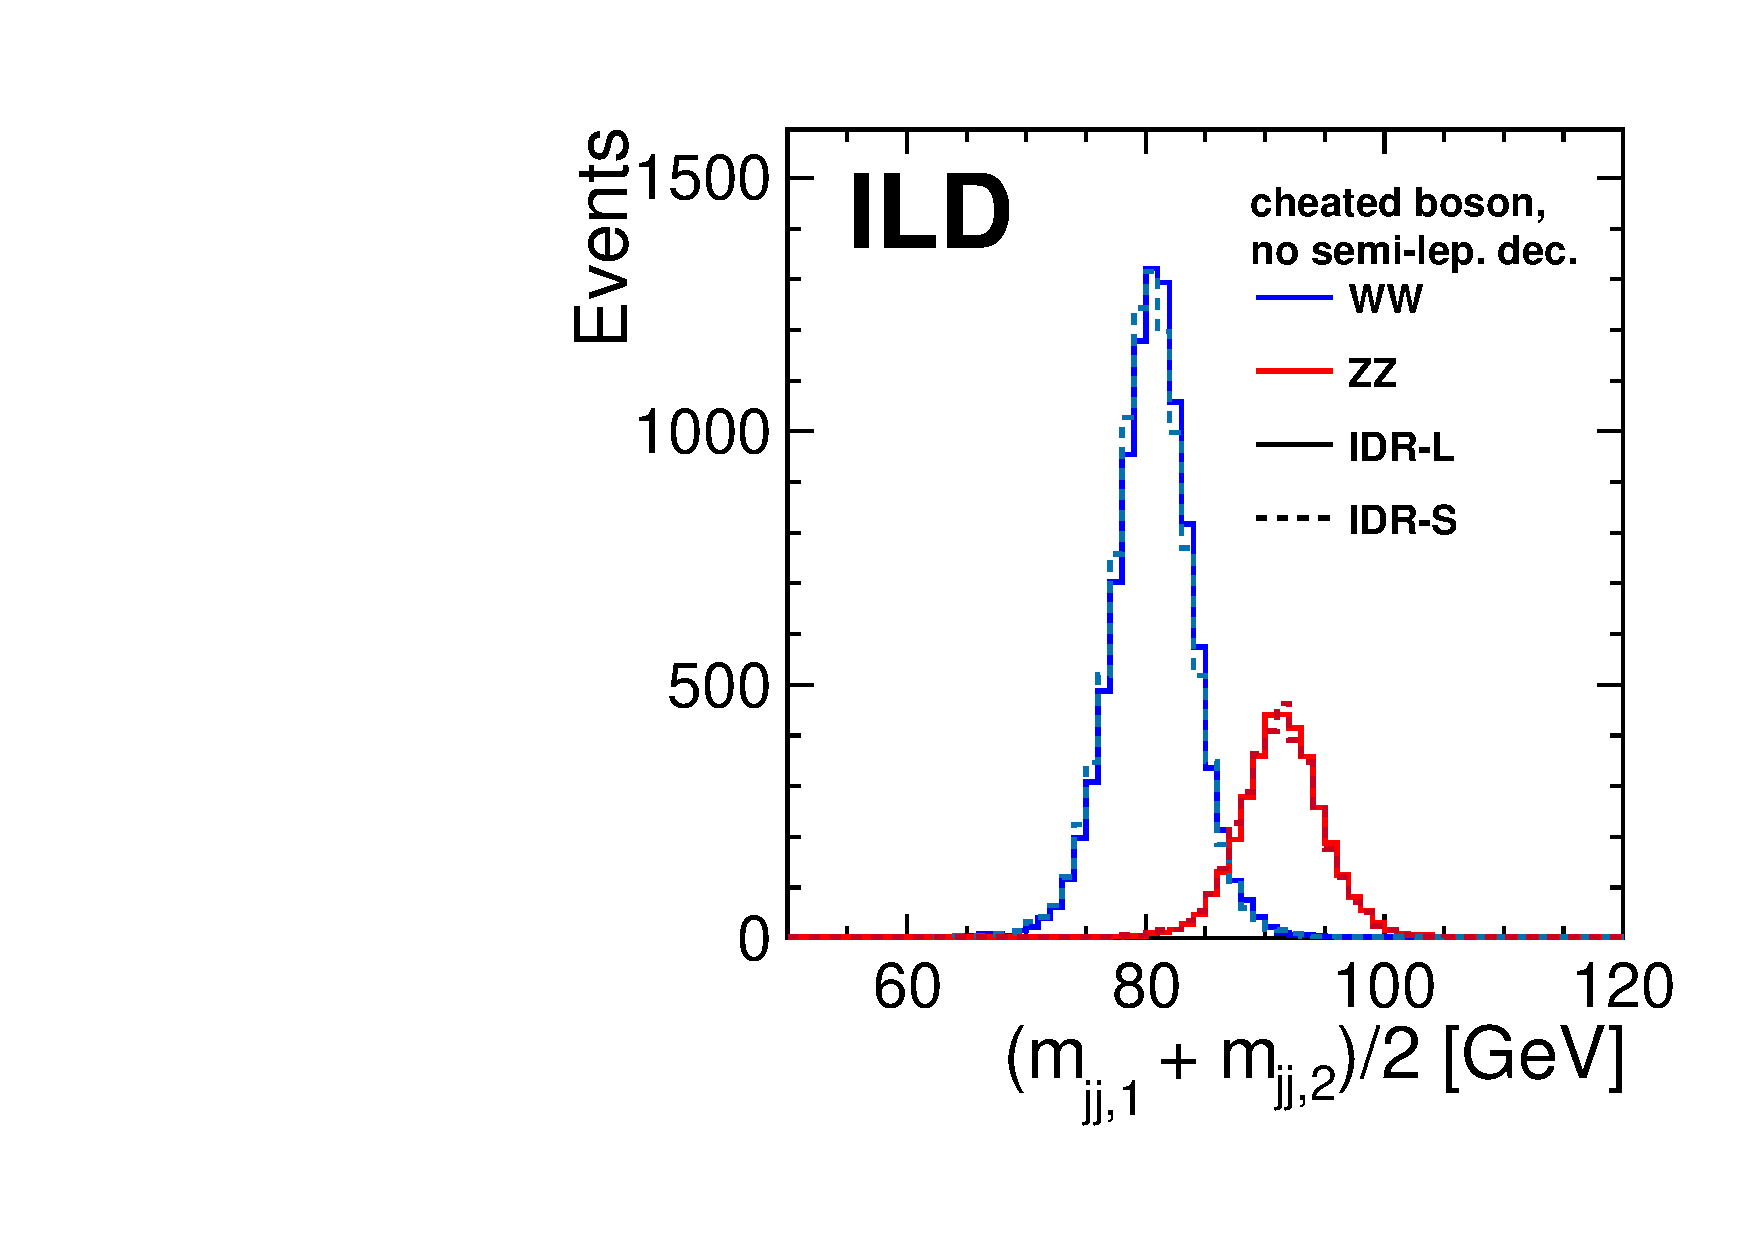
\includegraphics[width=\textwidth]{Performance/fig/ls_comp_icn_noSLD_monly.pdf}
 \caption{ \label{fig:qgc:cheat:1d}}
 \end{subfigure}
%\hspace{0.03\textwidth}
\begin{subfigure}{0.49\hsize} 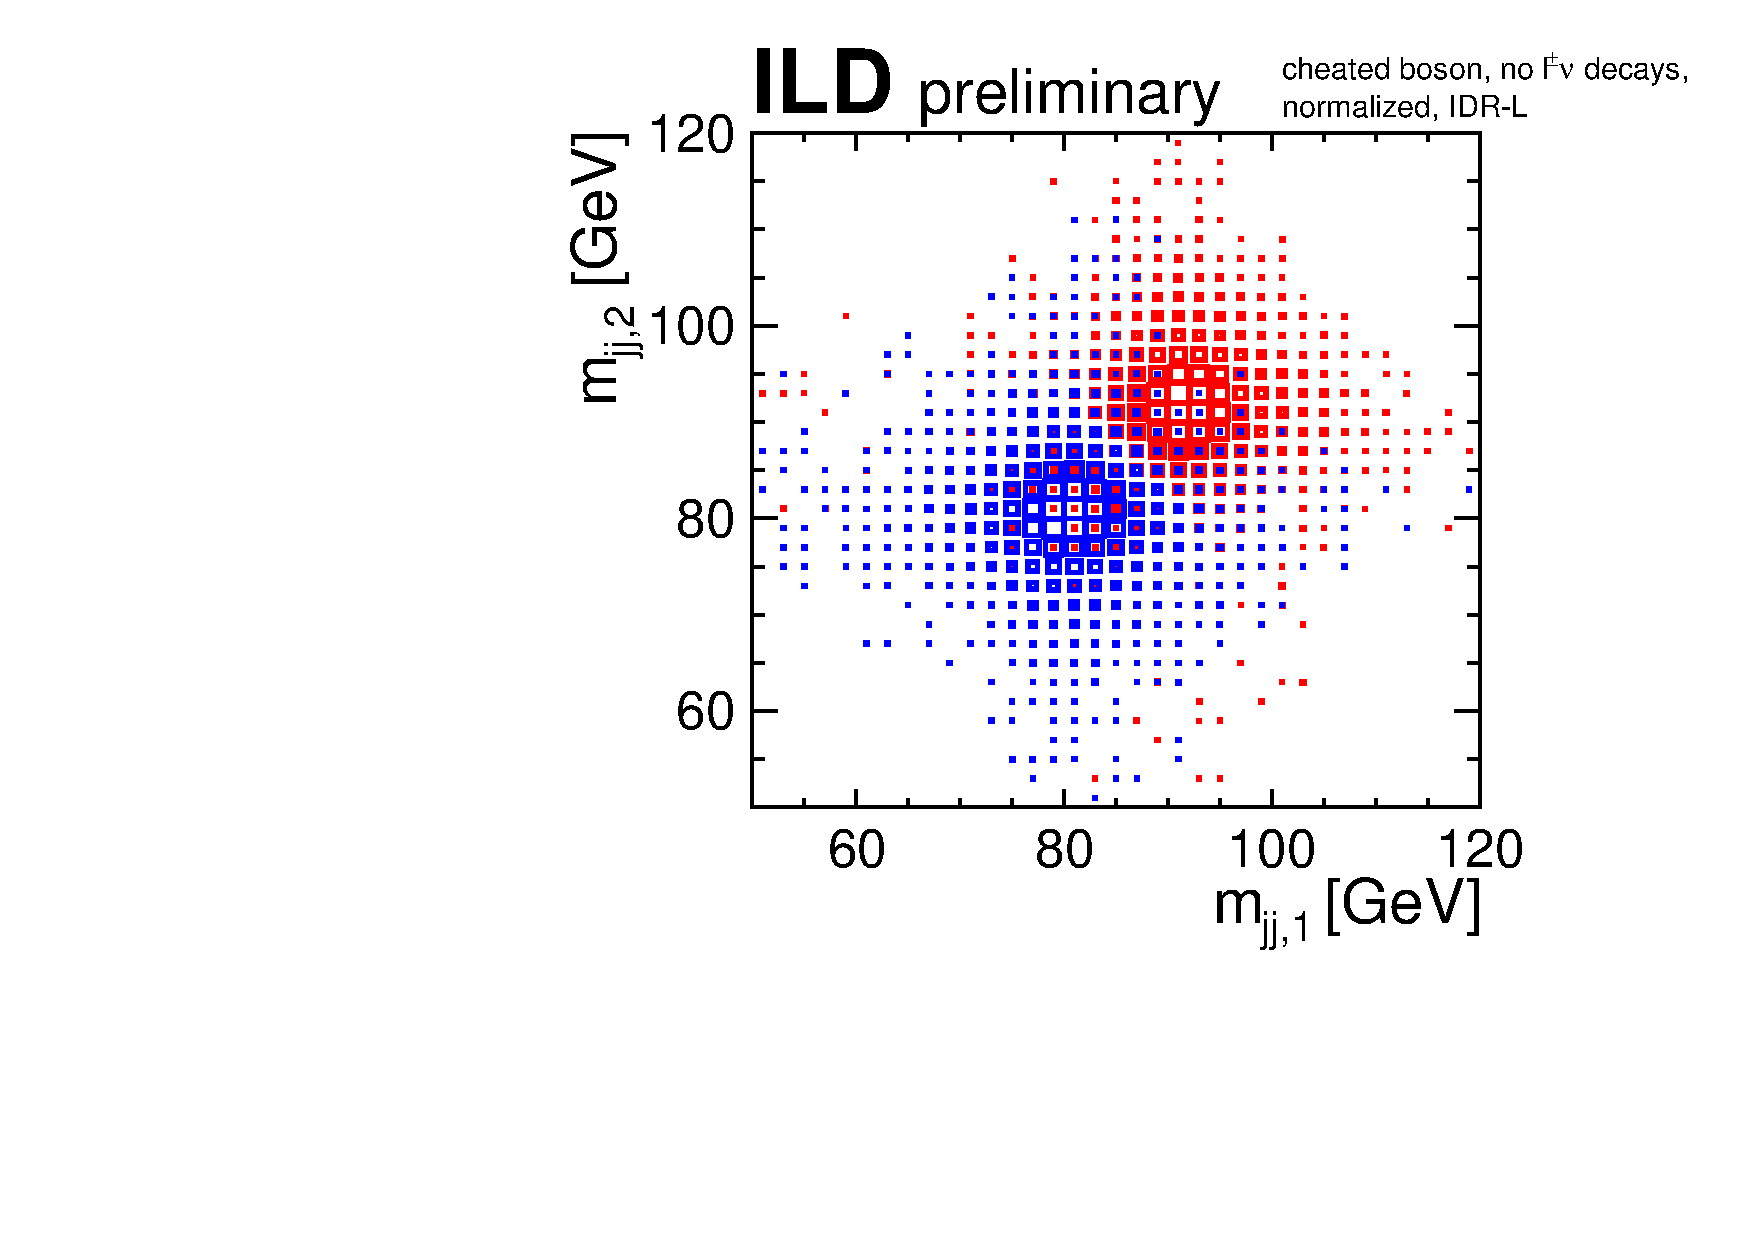
\includegraphics[width=\textwidth]{Performance/fig/m_m_icn_noSLD.pdf}
 \caption{  \label{fig:qgc:cheat:2d}}
 \end{subfigure}
%\end{center}
\caption{Dijet masses in $e^+e^- \to \nu\nu WW$ (blue) and $e^+e^- \to \nu\nu ZZ$ (red) events as obtained for ILC1000 as defined in Sec.~\ref{sec:benchmarks:lep} when cheating the jet clustering and excluding events where one (or more) jets contain semi-leptonic charm or beauty decays.
(a) Average of the two di-jet masses per event. 
(b) 2D illustration of the two di-jet masses per event.
}
\label{fig:qgc:cheat}
\end{figure}


\begin{figure}[htbp]
\begin{center}
\begin{subfigure}{0.495\hsize} 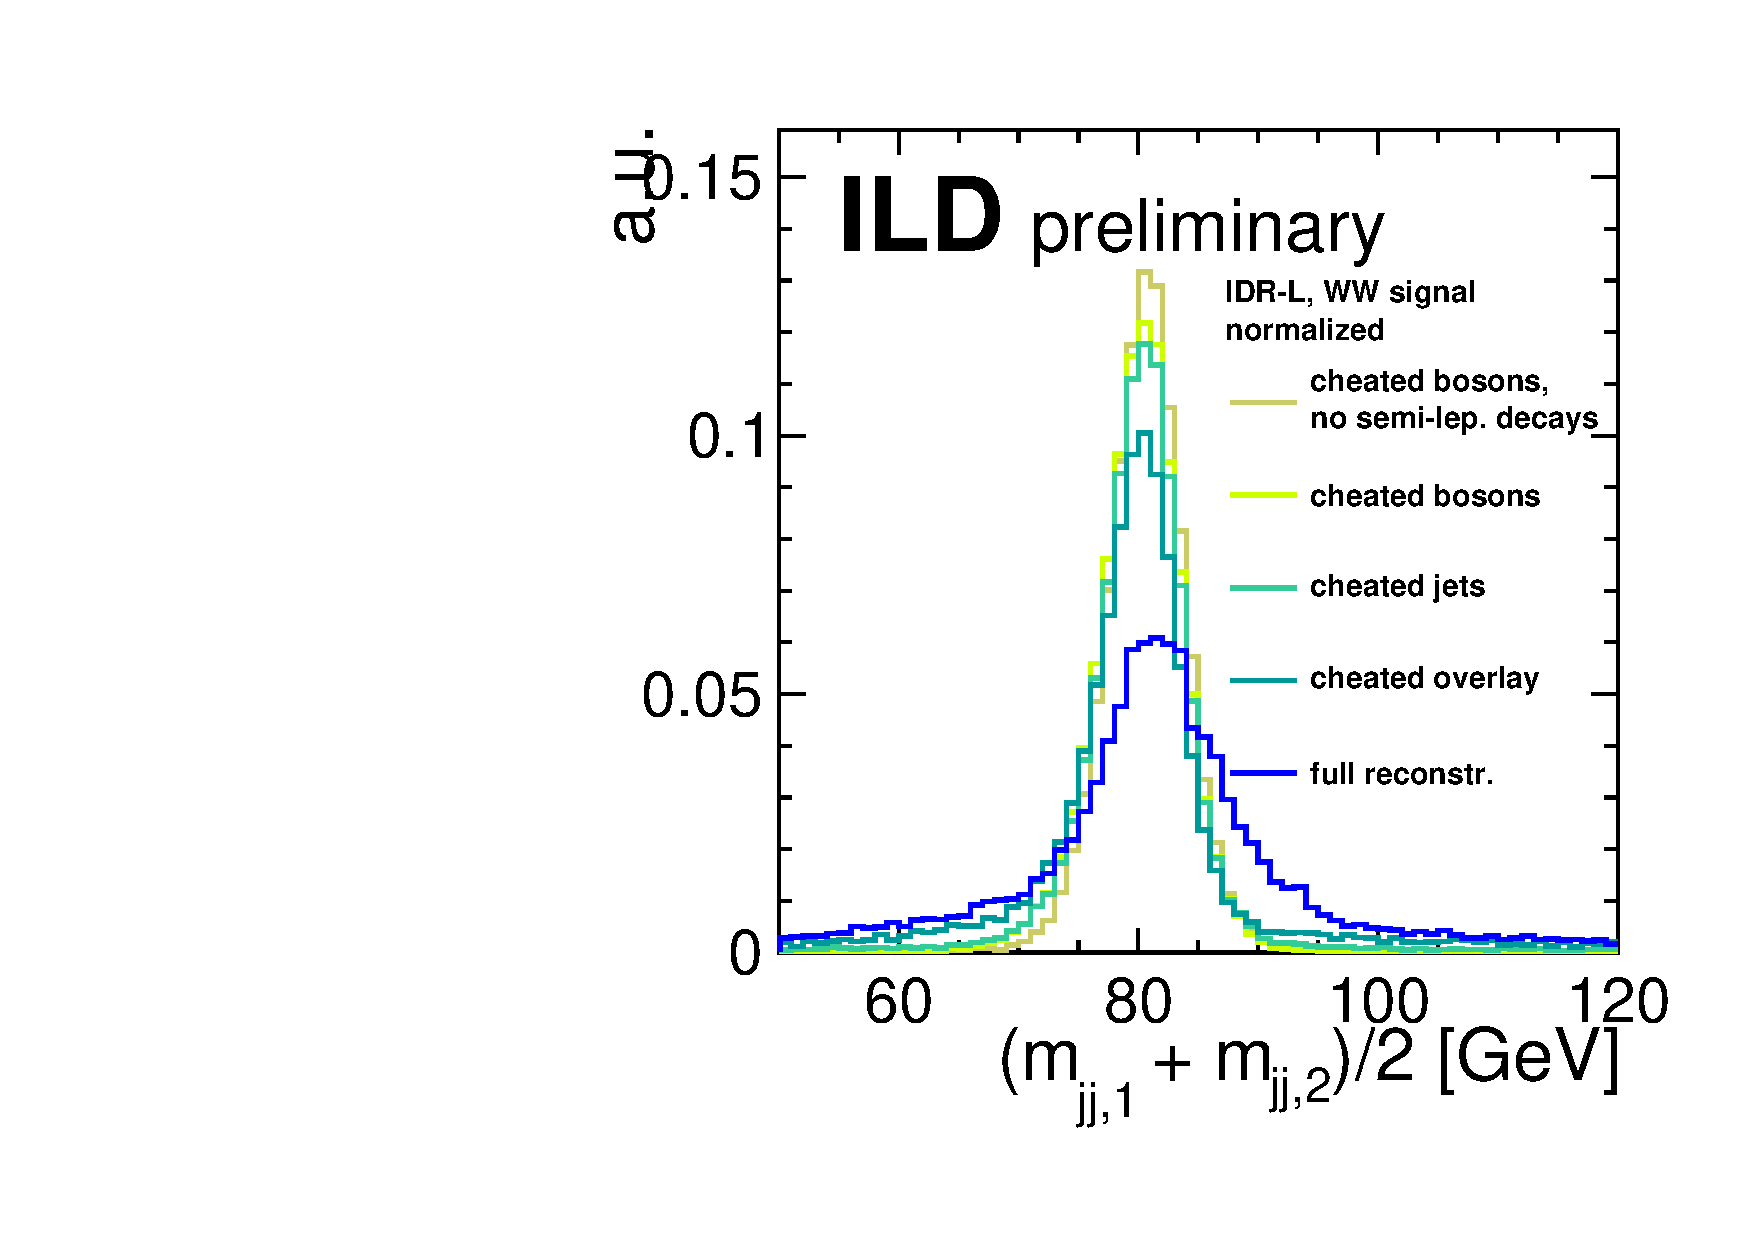
\includegraphics[width=\textwidth]{Performance/fig/l_WW_cheating_steps.pdf}
 \caption{ \label{fig:qgc:cheat:WW}}
 \end{subfigure}
%\hspace{0.03\textwidth}
\begin{subfigure}{0.495\hsize} 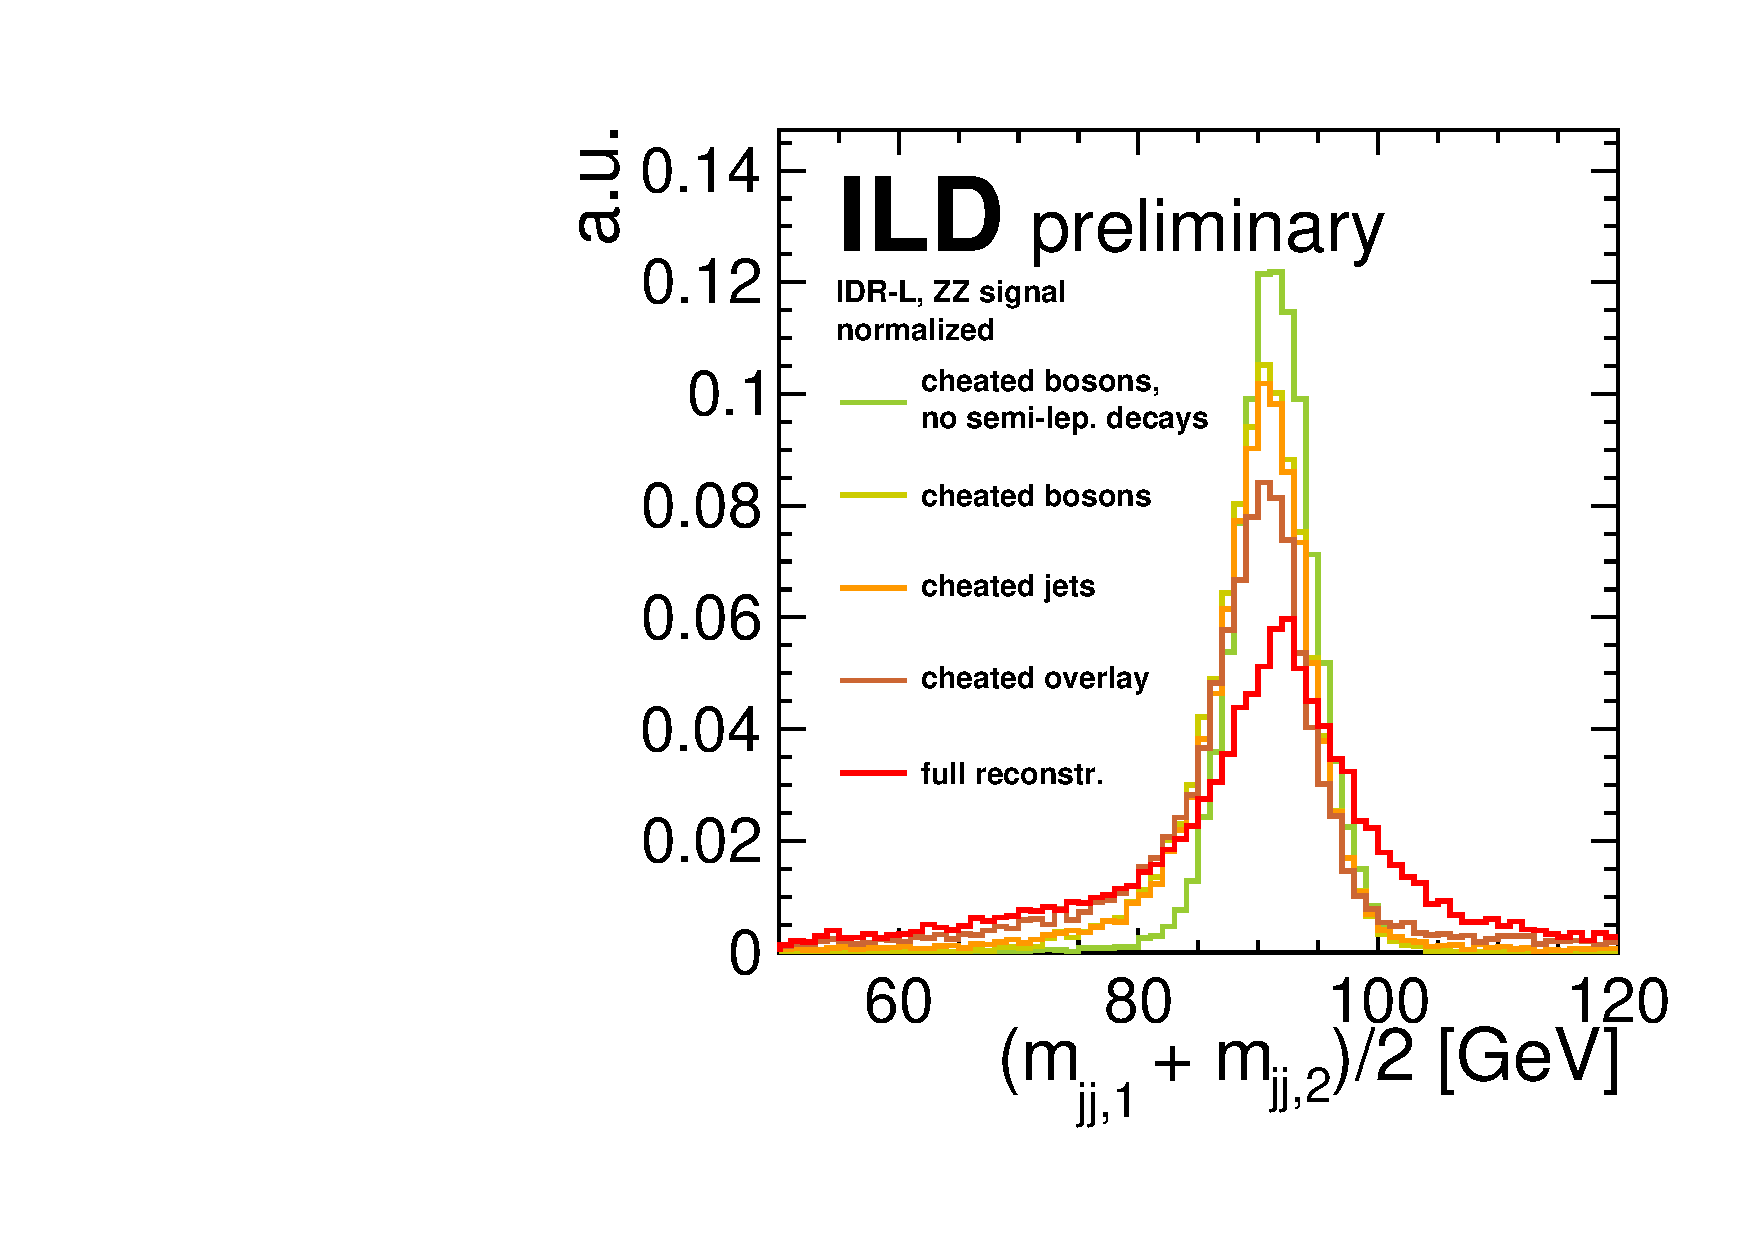
\includegraphics[width=\textwidth]{Performance/fig/l_ZZ_cheating_steps.pdf}
 \caption{  \label{fig:qgc:cheat:ZZ}}
 \end{subfigure}
%\end{center}
\begin{subfigure}{0.495\hsize} 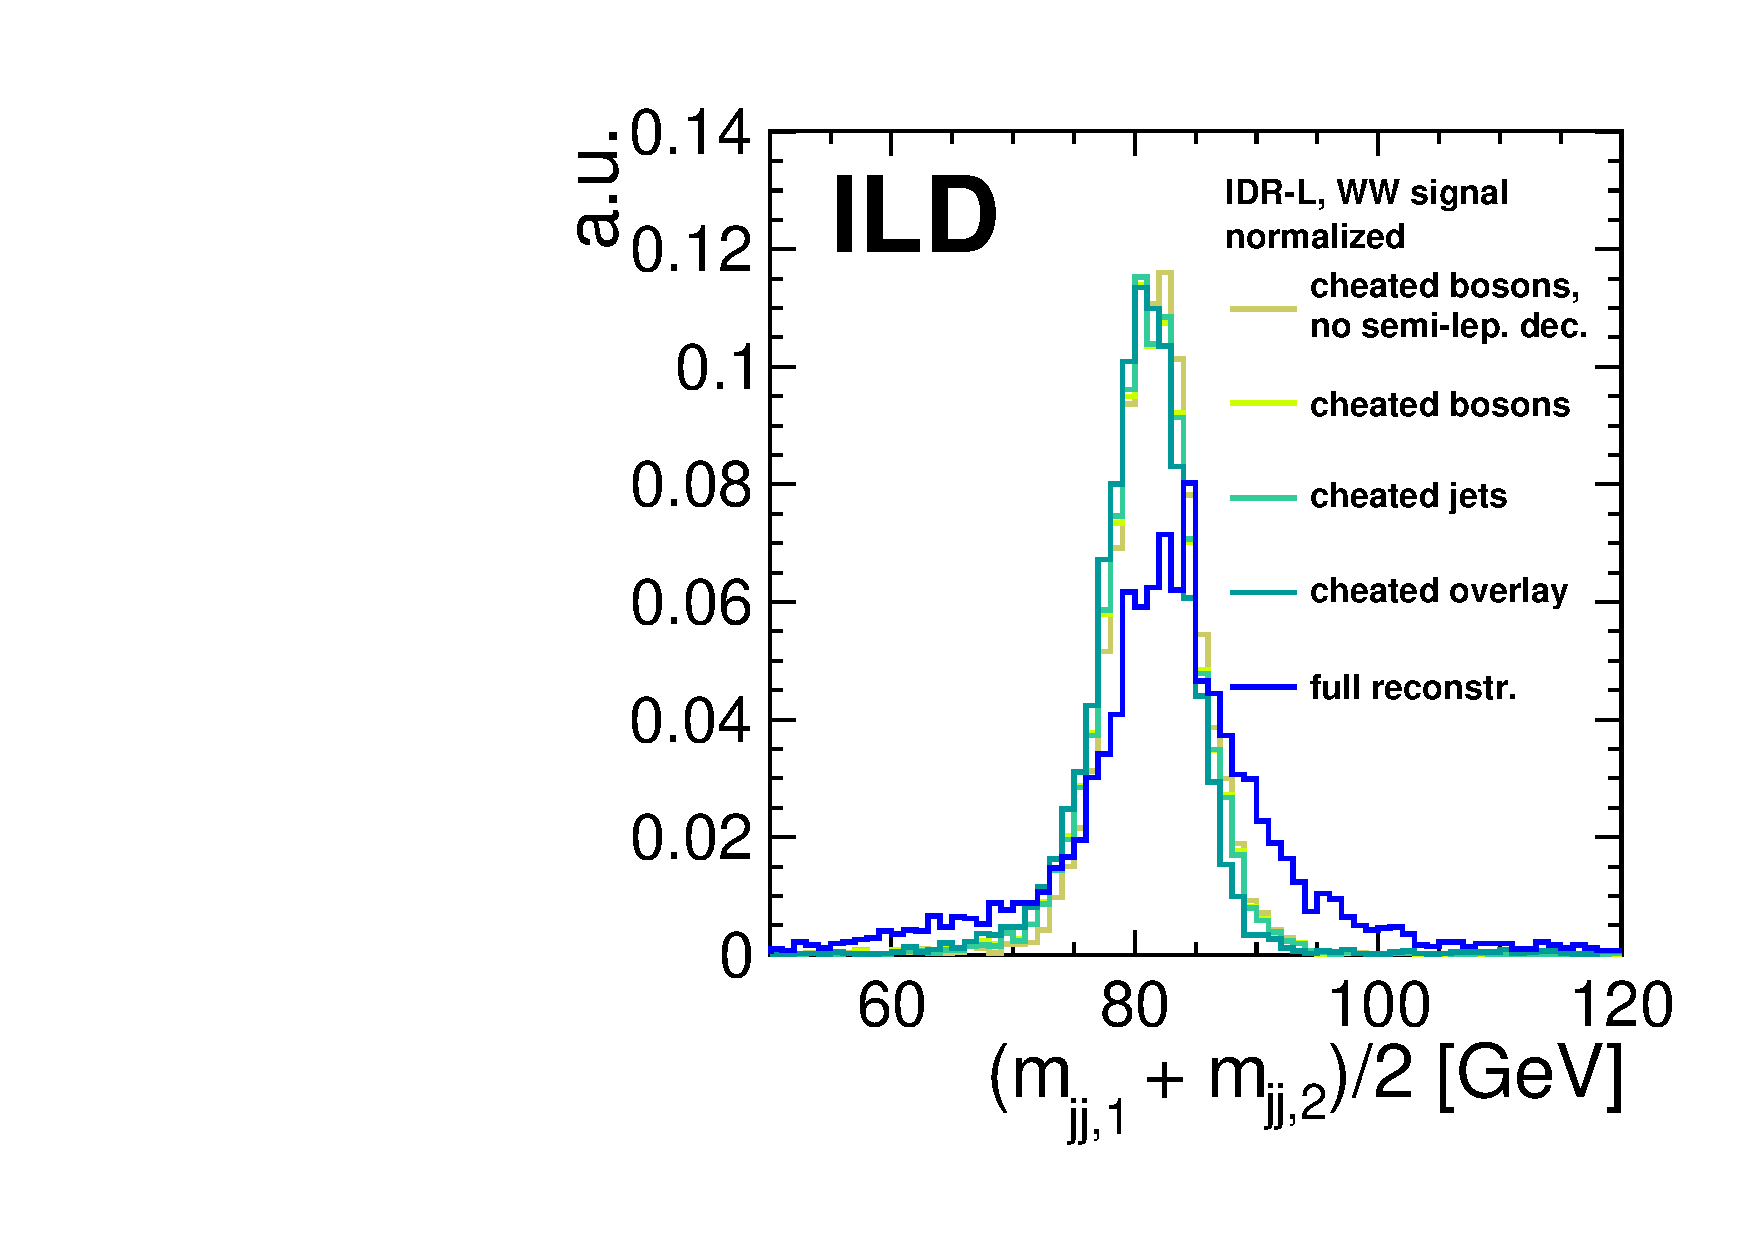
\includegraphics[width=\textwidth]{Performance/fig/l_WW_cheating_steps_highQ2.pdf}
 \caption{ \label{fig:qgc:cheat:WWQ2}}
 \end{subfigure}
%\hspace{0.03\textwidth}
\begin{subfigure}{0.495\hsize} 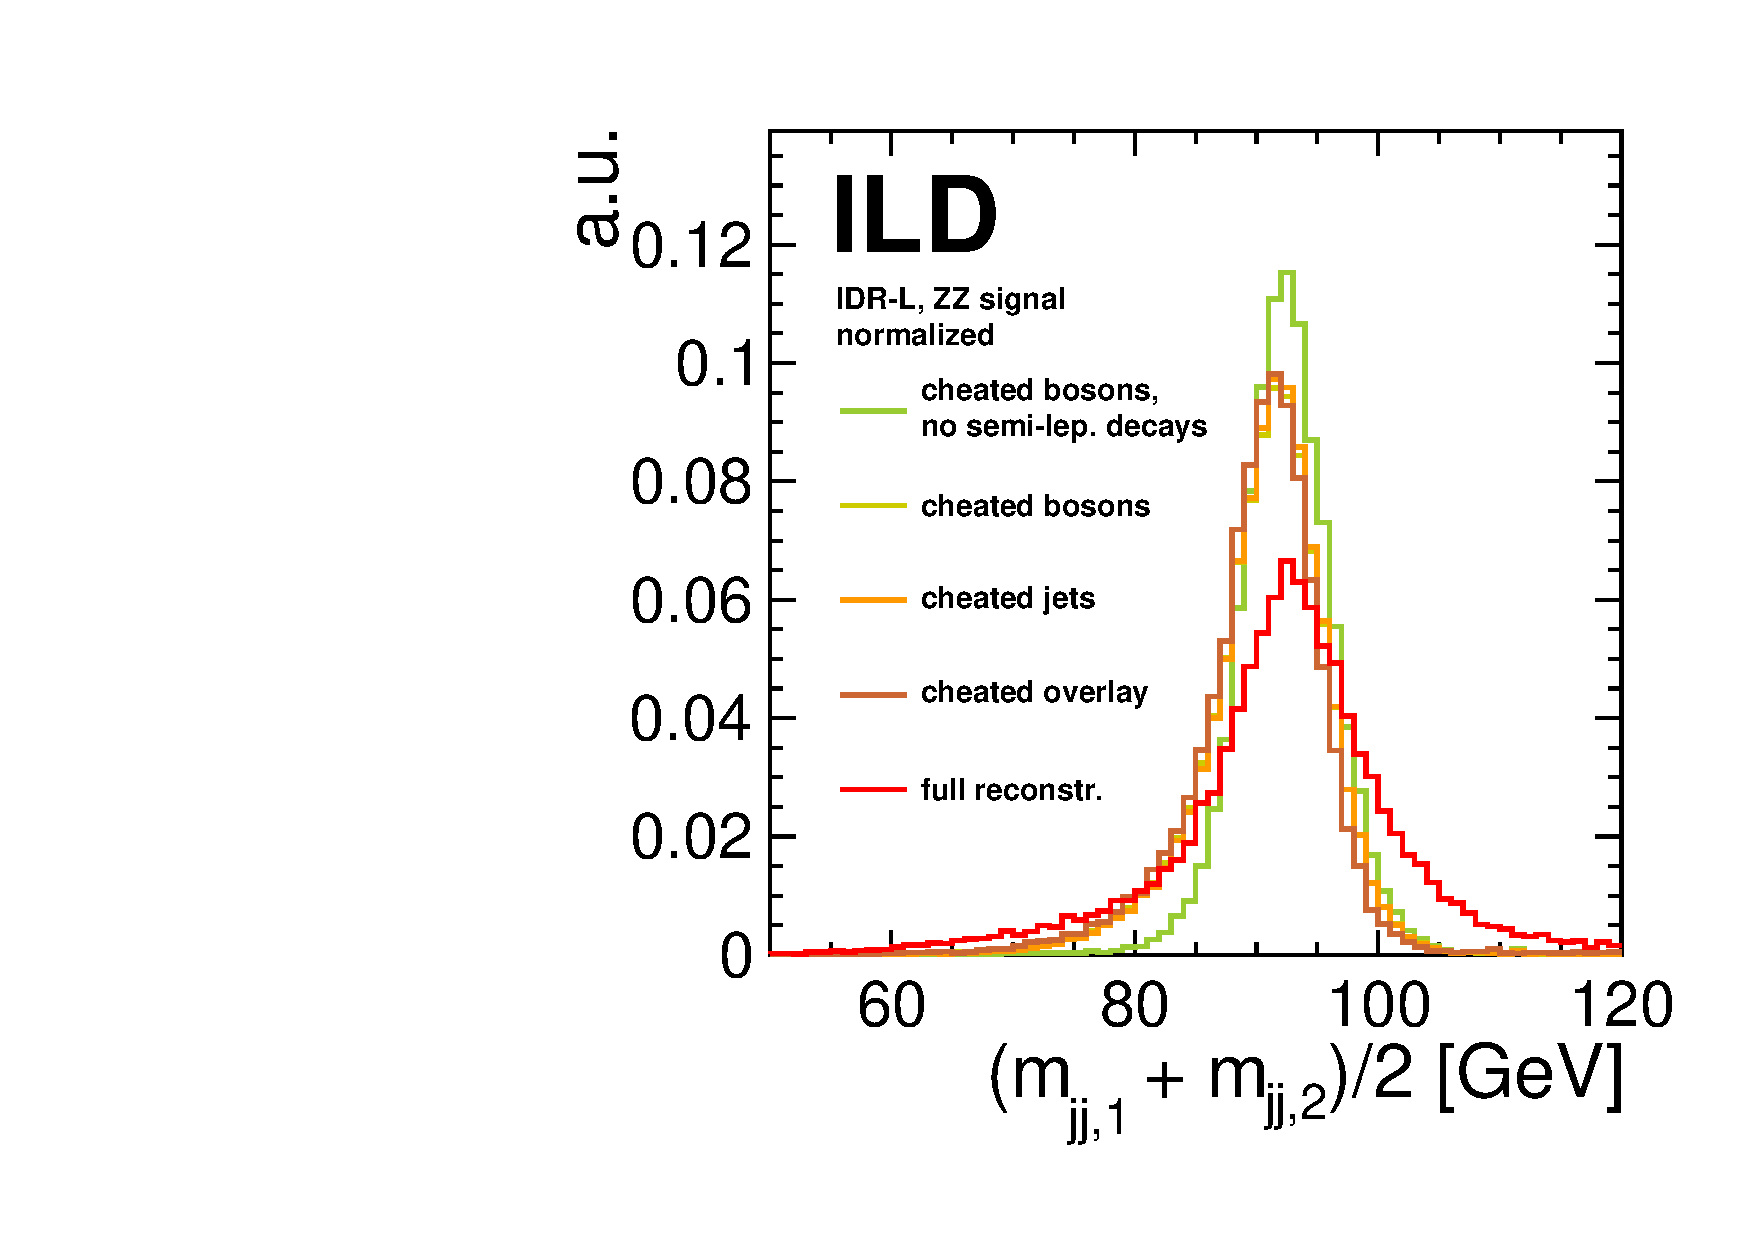
\includegraphics[width=\textwidth]{Performance/fig/l_ZZ_cheating_steps_highQ2.pdf}
 \caption{  \label{fig:qgc:cheat:ZZQ2}}
 \end{subfigure}
\end{center}
\caption{Average di-jet masses as obtained in full reconstruction at various levels of cheating.\\
(a) inclusive $e^+e^- \to \nu\nu WW$ events. 
(b) inclusive $e^+e^- \to \nu\nu ZZ$ events.
(c)  $e^+e^- \to \nu\nu WW$ events with $M(WW)>500$\,GeV. 
(d)  $e^+e^- \to \nu\nu ZZ$ events with $M(ZZ)>500$\,GeV.\\
}
\label{fig:qgc:cheatWWZZ}
\end{figure}

Figure~\ref{fig:qgc:cheat} shows the analogous distributions obtained when cheating the jet clustering (incl.\ the overlay removal), the jet pairing and when excluding events with semi-leptonic decays of heavy quarks, so that only the effects of the natural widths of the bosons, of fragmentation and hadronisation as well as the JER itself remain. Also here, no striking difference between the models can be seen, which leads to the conclusion that on this event sample, which is dominated by events with rather low invariant masses of the di-boson system, the effect of the slightly worse JER of ILD-S is hidden beneath the width and fragmentation/hadronisation effects, since these are only remaining influences -- besides the JER -- in Fig.~\ref{fig:qgc:cheat}.


Nevertheless, the differences between Fig.~\ref{fig:qgc:rec} and Fig.~\ref{fig:qgc:cheat} are striking. Therefore, we investigated the impact of the size of various contributions individually as shown in Fig.~\ref{fig:qgc:cheatWWZZ}, for ILD-L only. For the inclusive $WW$ and $ZZ$ samples, shown in Figs.~\ref{fig:qgc:cheat:WW} and~\ref{fig:qgc:cheat:ZZ}, the dominant effect is the residual of the non-perfect overlay removal, followed by the jet clustering itself and the semi-leptonic decays. Non-perfect jet pairing only plays a minor role. This can be compared to the situation found when only considering events with high $WW$/$ZZ$ invariant masses, shown in Figs.~\ref{fig:qgc:cheat:WWQ2} and~\ref{fig:qgc:cheat:ZZQ2}. In this case, the impact of non-perfect jet clustering is reduced to a negligible level. Instead, the effect of the residual overlay from low-$p_t$ $\gamma \gamma \to $hadron events dominates. For the $ZZ$ events, also the missing neutrinos from semi-leptonic heavy quark decays play a visible role. 
These results demonstrate the need for development of more sophisticated high-level reconstruction algorithms, in particular for the overlay removal, the jet clustering and the identification and correction of semi-leptonic heavy flavour decays. For all these cases promising tools are under development, see e.g.\ Sec.~\ref{subsec:bench:higgsino} and Ref.~\cite{Boronat:2014hva}.

%%%%%%%%%%%%%%%%%%%%%%%%%%%%%%%%%%%%%%%%%%%%%%%%%%%%%%%%%%%%%%%%%%%
\subsection{Photon Energy Scale Calibration from \texorpdfstring{$e^+e^- \to \gamma Z \to \gamma \mu^+\mu^-$}{e+e- -> aZ -> mumu}}
\label{subsec:bench:gammaZ}
%%%%%%%%%%%%%%%%%%%%%%%%%%%%%%%%%%%%%%%%%%%%%%%%%%%%%%%%%%%%%%%%%%%

Di-fermion production, with or without radiative return to the $Z$ pole, is an integral part of the ILC physics case. In addition, the radiative return events offer an important
opportunity to cross calibrate the energy scales of various subdetectors. As a detector benchmark, we chose here the example of calibrating the photon energy scale against the momentum scale of the tracker. Thereby, the momenta and angles of the muons as well as the 
polar and azimuthal angle of the photon serve as input from which the energy of the photon and the amount of energy lost in beamstrahlung and collinear ISR are determined by
requiring conservation of energy and $p_y$ between initial and final state. It should be stressed that it is not necessary to apply a $Z$ mass constraint, which would introduce an additional uncertainty due to the large natural width of the $Z$ resonance. A full description of this and alternative methods can be found in~\cite{ILDNote:gammaZ}.
 

\begin{figure}[htbp]
\begin{subfigure}{0.49\hsize} 
 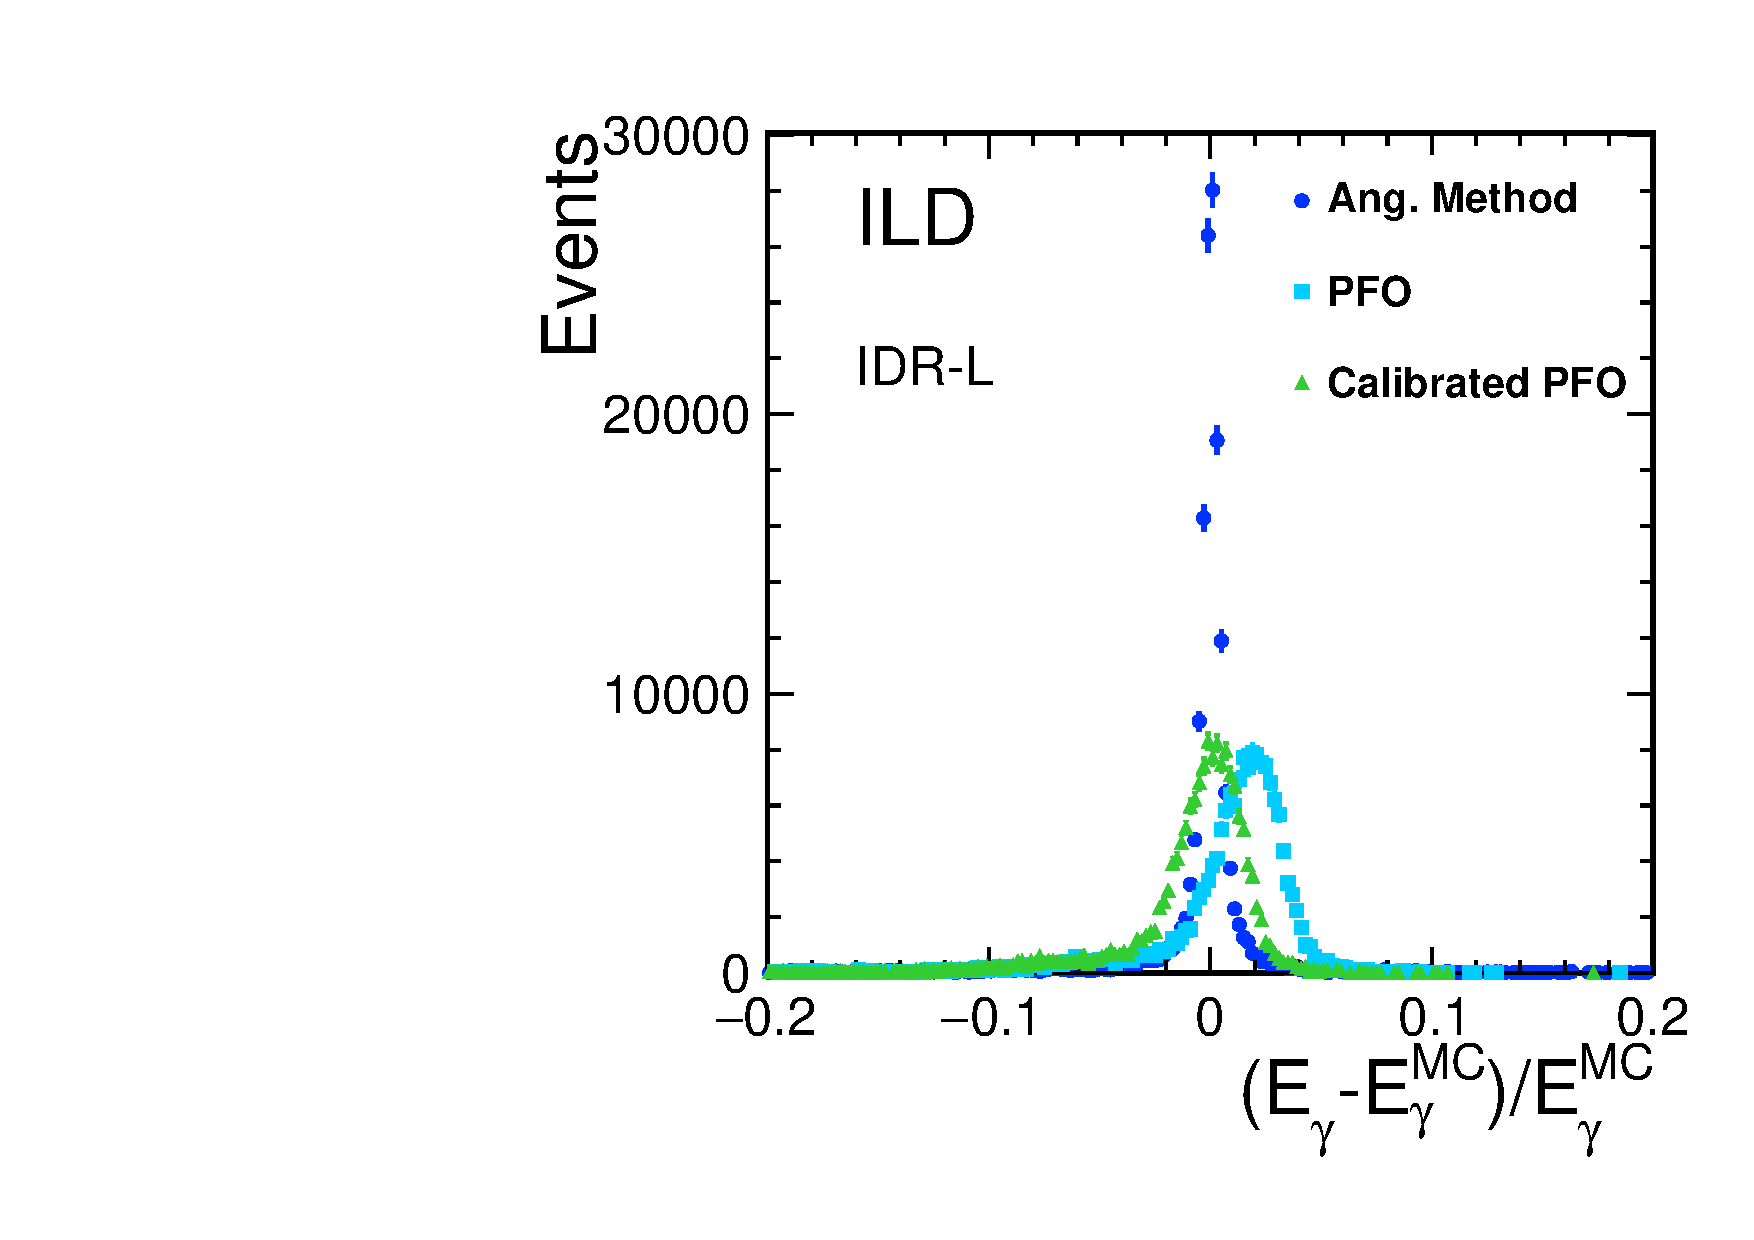
\includegraphics[width=\textwidth]{Performance/fig/IDR1MethodComp.pdf}
 \caption{ \label{fig:gammaZ:meanE:allE}}
 \end{subfigure}
\begin{subfigure}{0.49\hsize} 
 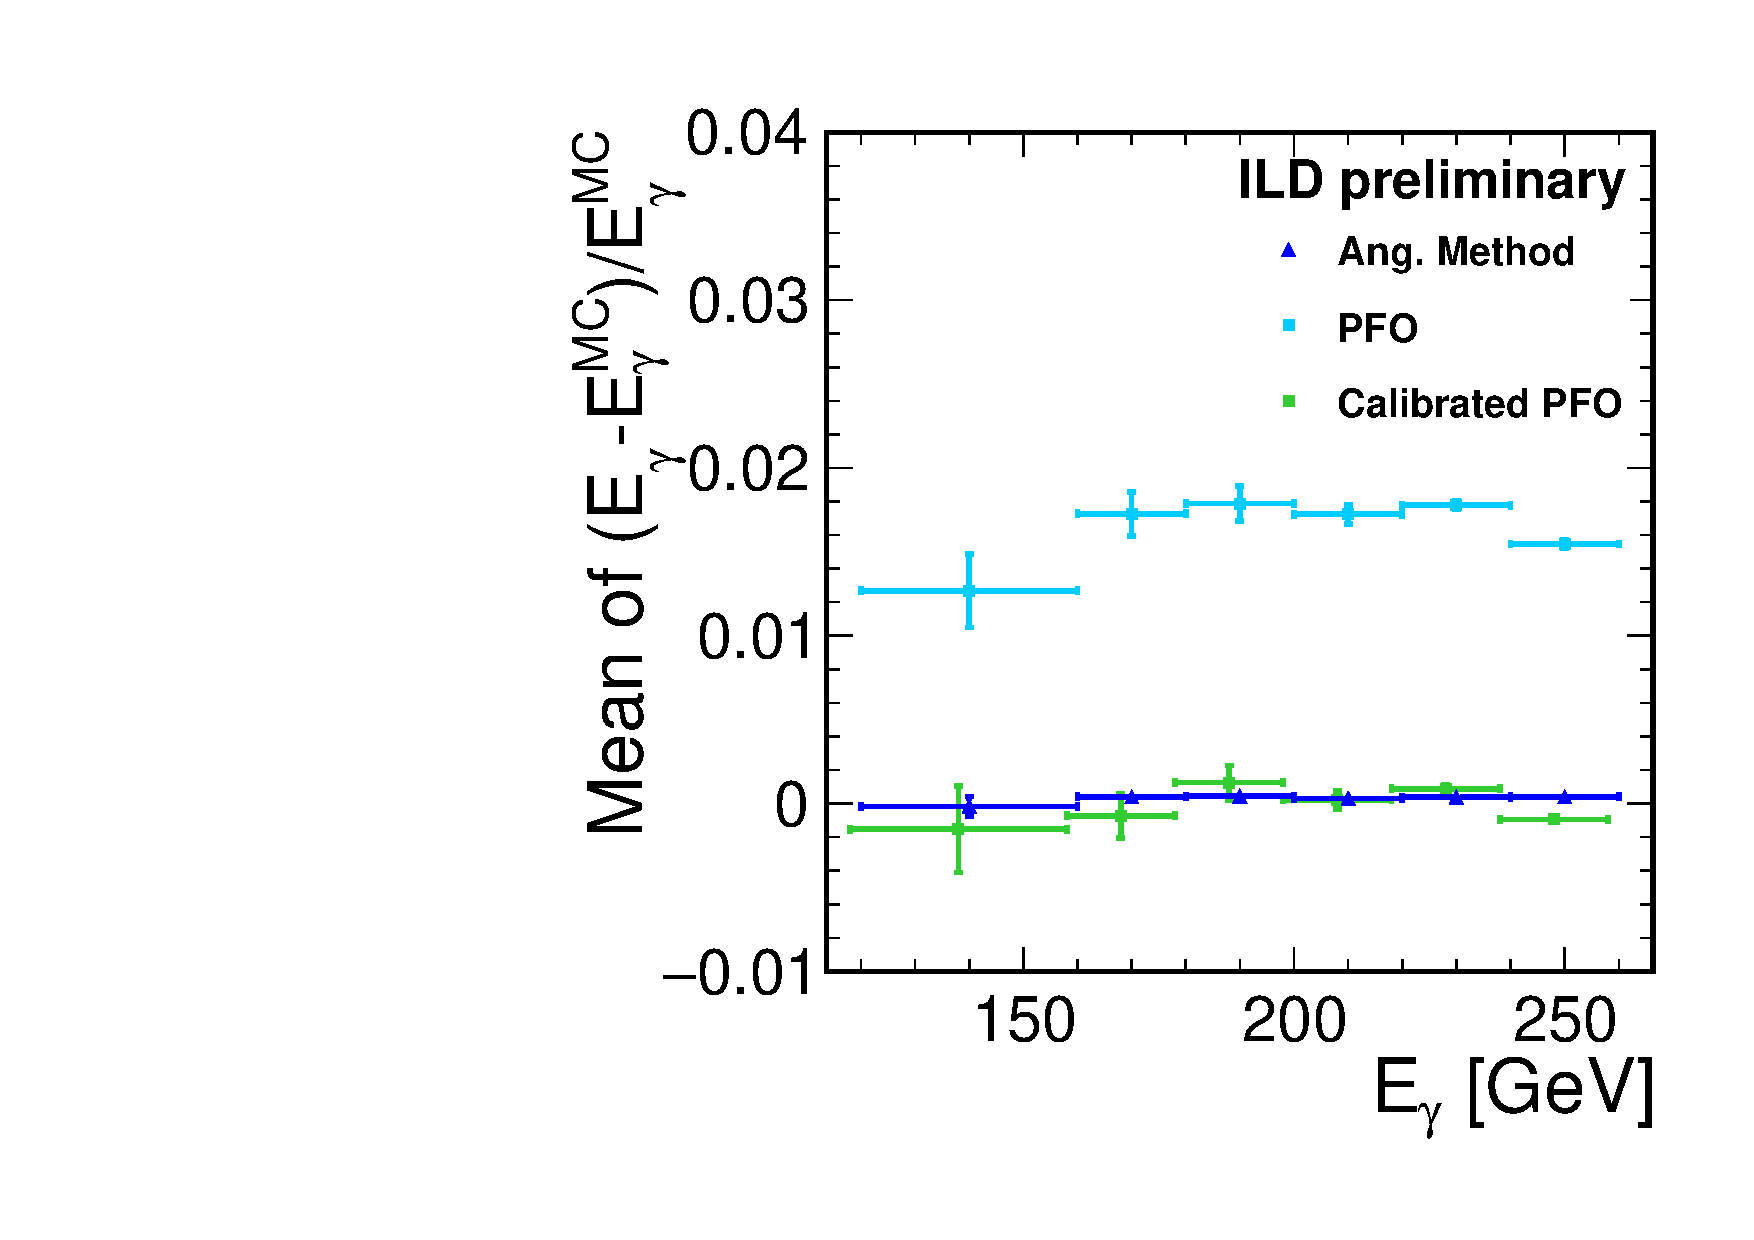
\includegraphics[width=\textwidth]{Performance/fig/IDR5ECentervalueE.pdf}
 \caption{  \label{fig:gammaZ:meanE:vsE}}
 \end{subfigure}
\caption{
Deviation of the photon energy from its true value when using non-perfectly calibrated PFO-level energies (cyan), when calculating the photon energy from the $\mu$ momenta and kinematic constraints (blue, ``angular method'') and after calibrating the mean PFO-level w.r.t.\ the mean obtained from the $\mu$ momenta (green).  
(a) Distribution of deviation for all photons in the sample.
(b) Mean deviation in bins of the photon energy.
}
\label{fig:gammaZ:meanE}
\end{figure}

Figure~\ref{fig:gammaZ:meanE} illustrates the power of this method by application to a non-perfectly calibrated photon reconstruction in the large detector model, both inclusively for all photons (Fig.~\ref{fig:gammaZ:meanE:allE}) and in bins of the photon energy (Fig.~\ref{fig:gammaZ:meanE:vsE}). Since the $e^+e^- \to \mu^+\mu^-\gamma$ sample
is dominated by radiative returns to the $Z$ pole, the majority of photons has high energies close to $241$\,GeV.

\begin{figure}[htbp]
\begin{subfigure}{0.49\hsize} 
 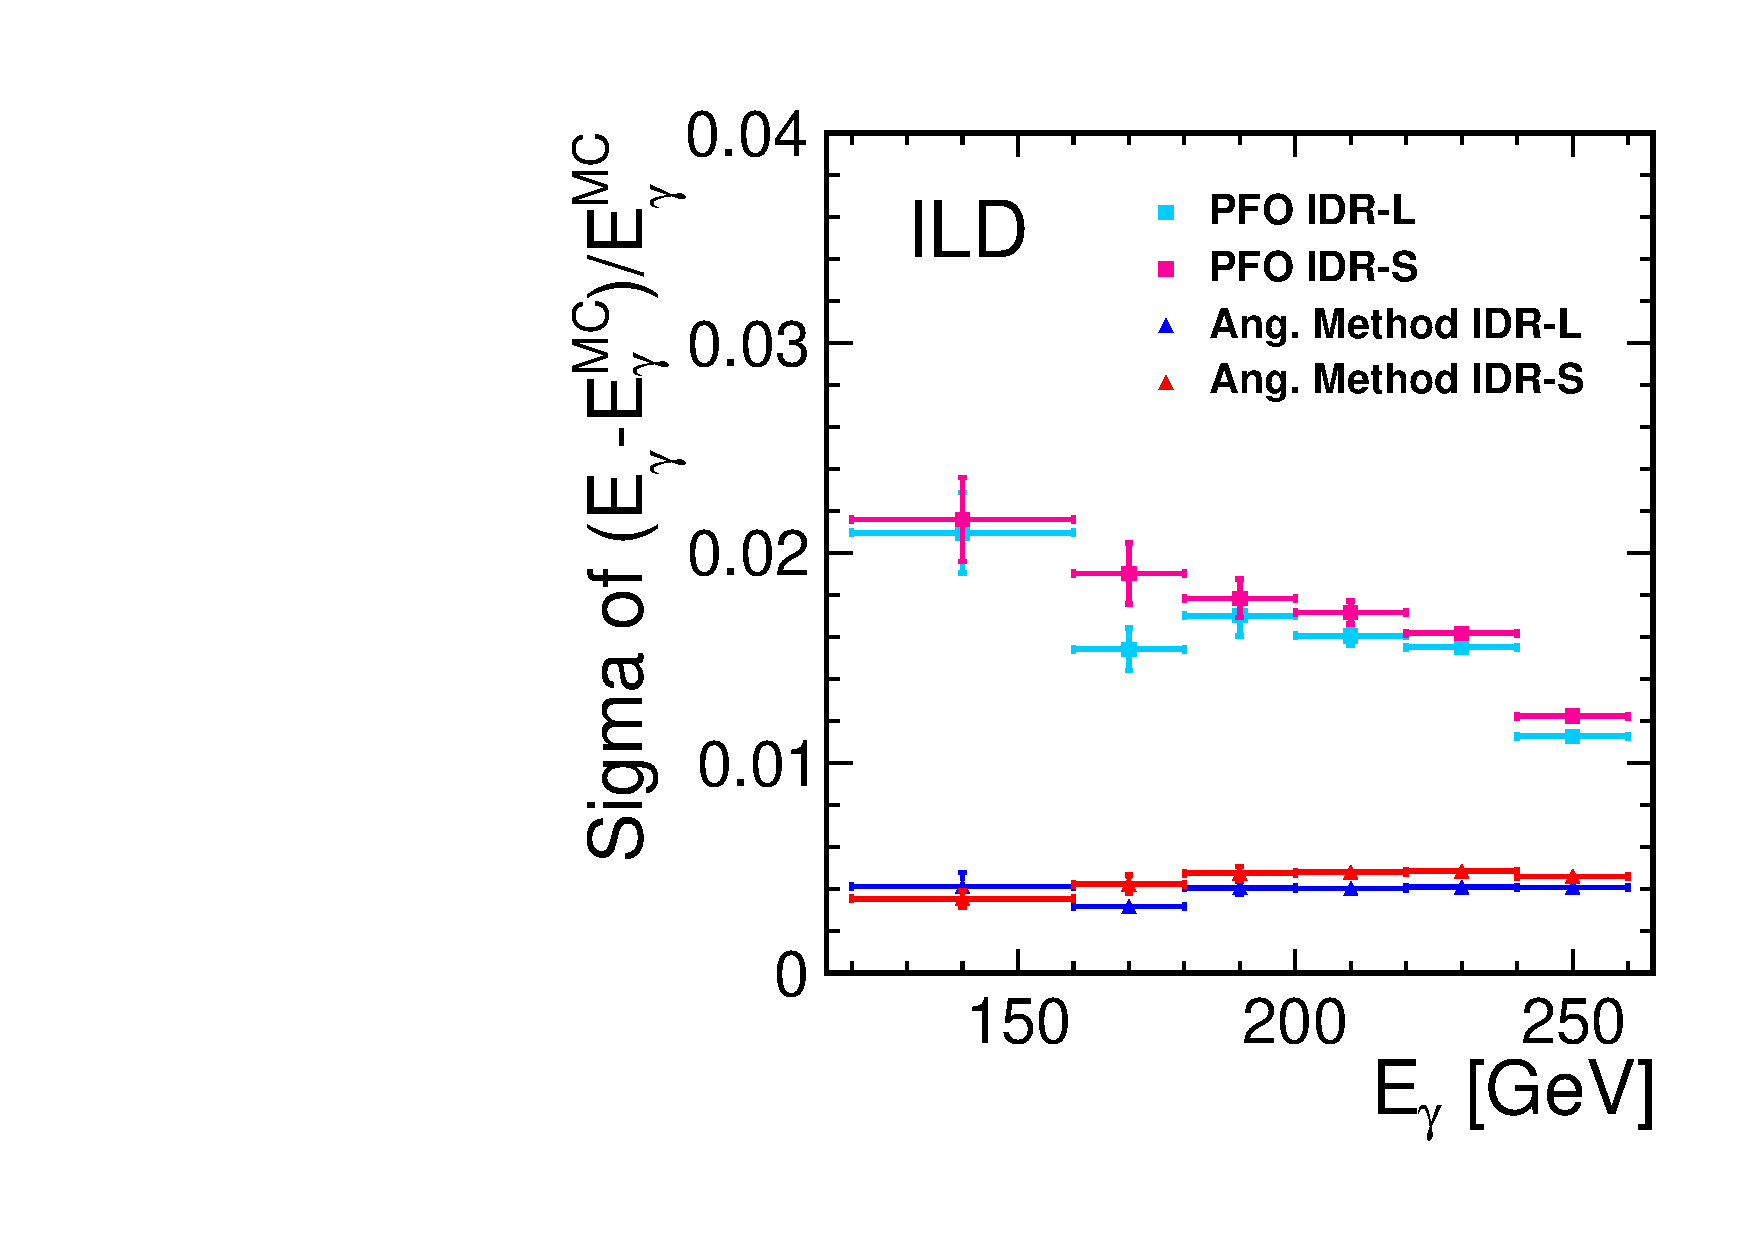
\includegraphics[width=\textwidth]{Performance/fig/IDR4EResolutionE.pdf}
 \caption{ \label{fig:gammaZ:sigmaE:rel}}
 \end{subfigure}
\begin{subfigure}{0.49\hsize} 
 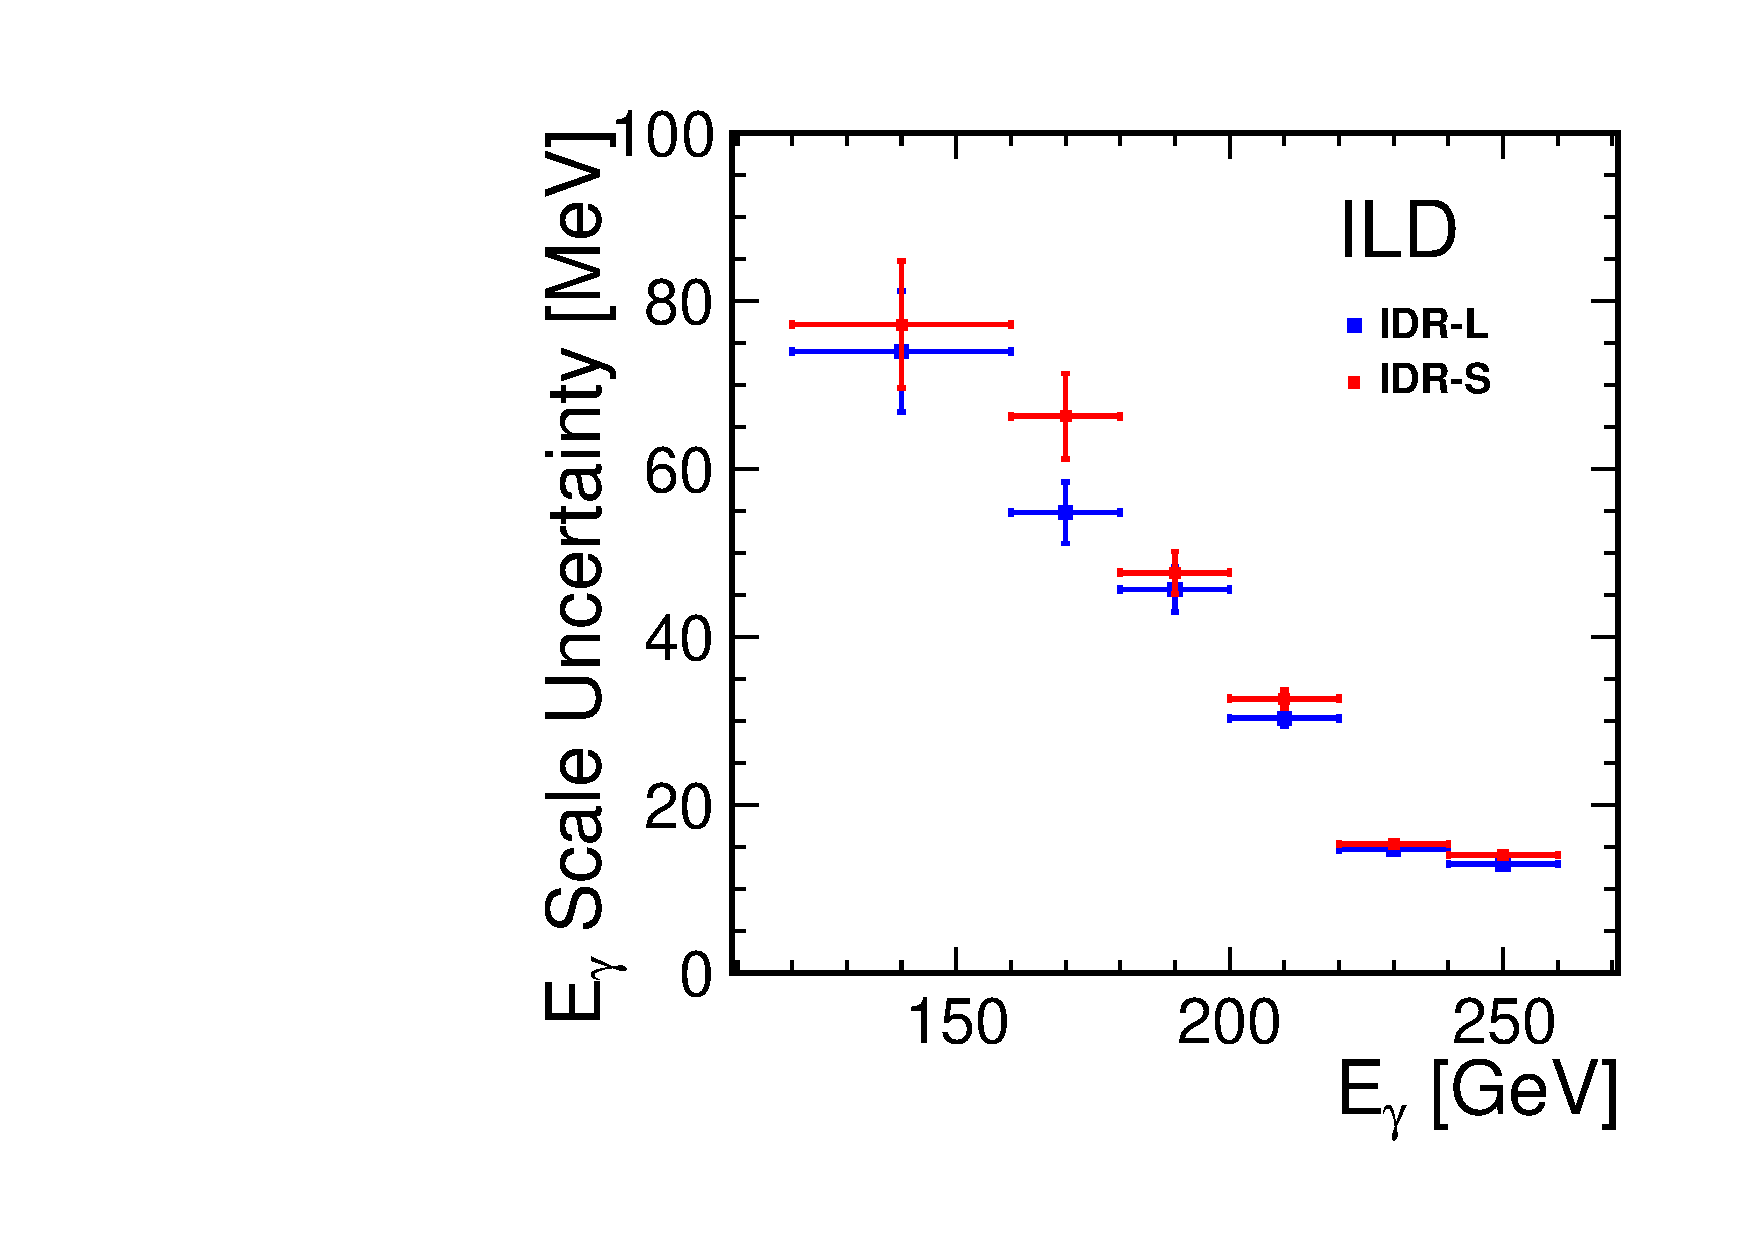
\includegraphics[width=\textwidth]{Performance/fig/IDR6EScaleUncertainty.pdf}
 \caption{  \label{fig:gammaZ:sigmaE:abs}}
 \end{subfigure}
\caption{Uncertainty on the photon energy scale calibration as a function of the photon energy for IDR-L and IDR-S.
(a) Relative uncertainty when using non-perfectly calibrated PFO-level energies (cyan/magenta) and when calculating the photon energy from the $\mu$ momenta and kinematic constraints (blue/red, ``angular method'').
(b) Absolute uncertainty from the angular method in MeV.
}
\label{fig:gammaZ:sigmaE}
\end{figure}

\begin{figure}[htbp]
\begin{subfigure}{0.49\hsize} 
 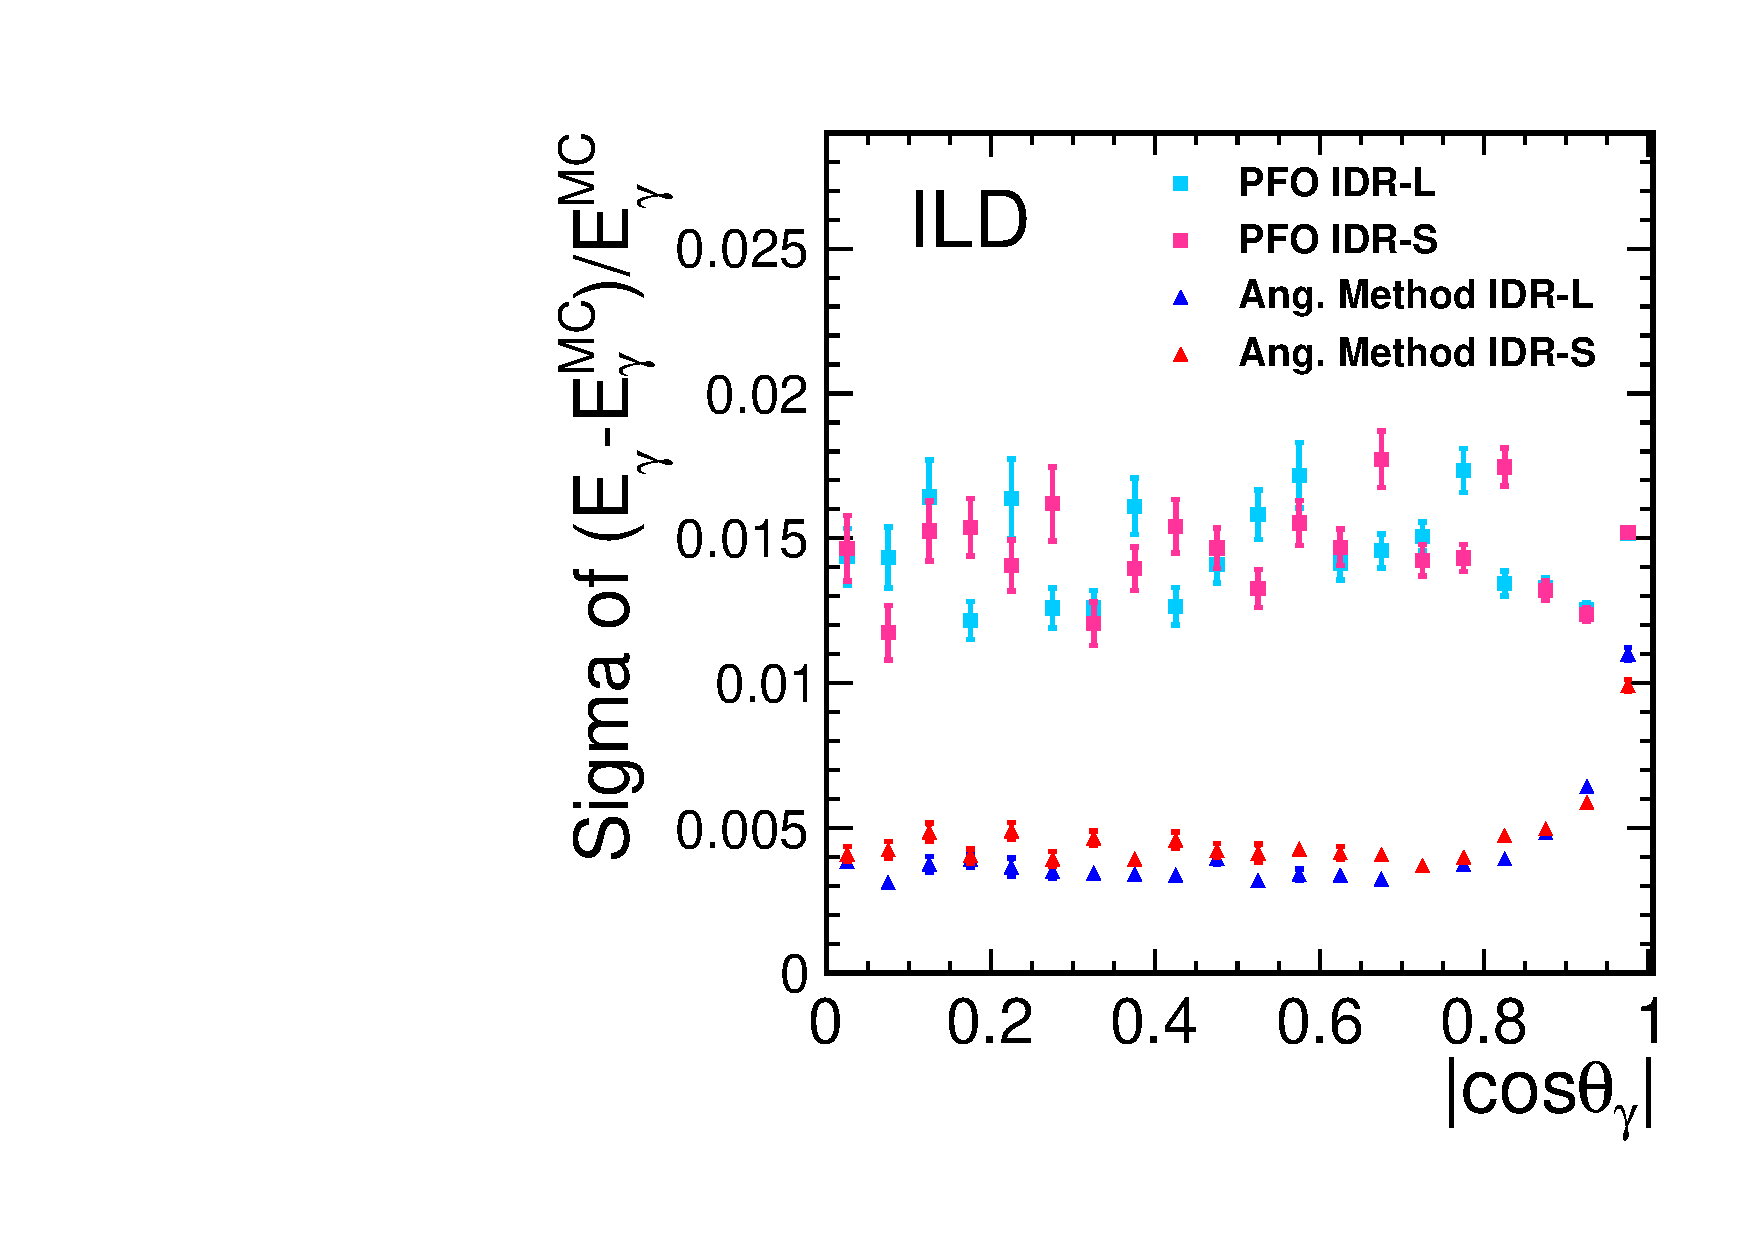
\includegraphics[width=\textwidth]{Performance/fig/IDR2EResolutionTheta.pdf}
 \caption{ \label{fig:gammaZ:angles:theta}}
 \end{subfigure}
\begin{subfigure}{0.49\hsize} 
 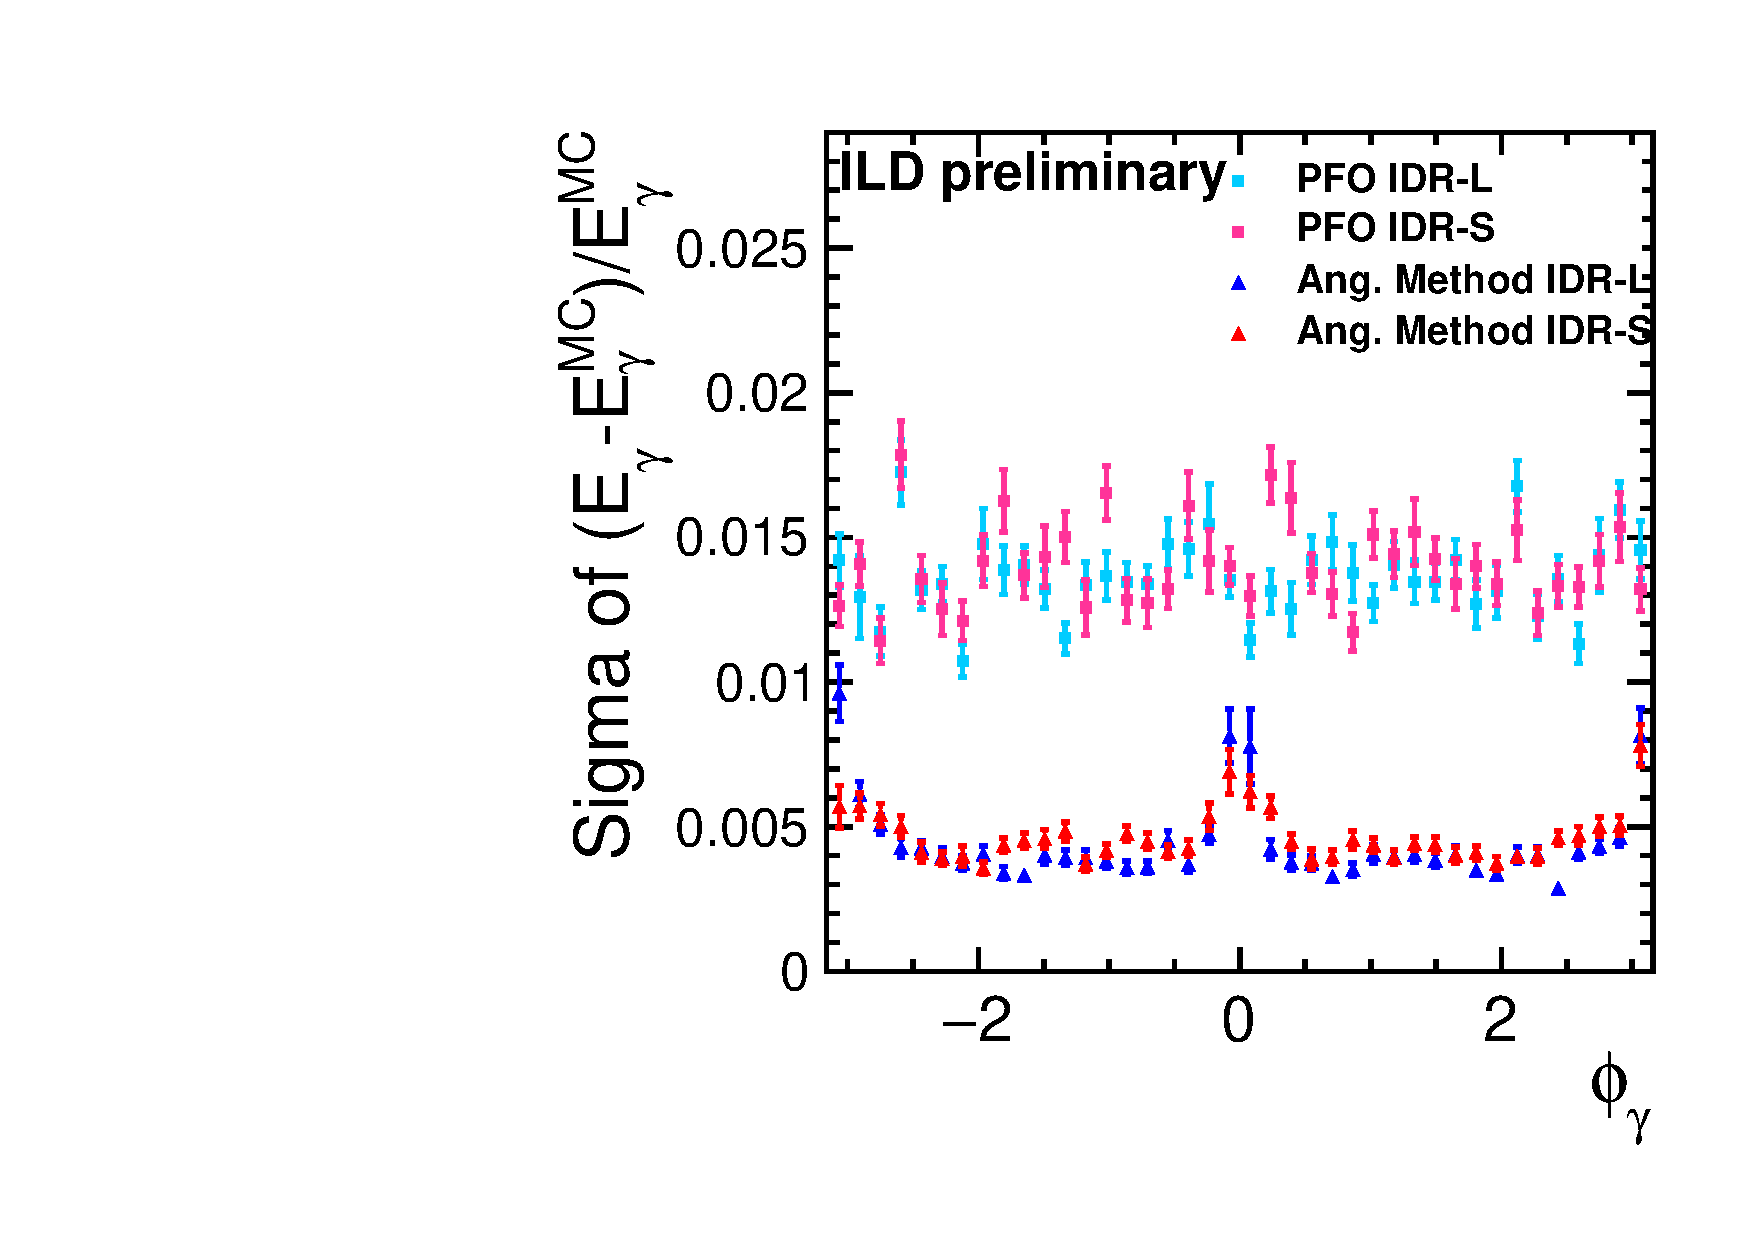
\includegraphics[width=\textwidth]{Performance/fig/IDR3EResolutionPhi.pdf}
 \caption{  \label{fig:gammaZ:angles:phi}}
 \end{subfigure}
\caption{
Resolution of the photon energy when using non-perfectly calibrated PFO-level energies (cyan/magenta) and when calculating the photon energy from the $\mu$ momenta and kinematic constraints (blue/red, ``angular method'').  
(a) as a function of the polar angle
(b) as a function of the azimuthal angle
}
\label{fig:gammaZ:angles}
\end{figure}

The resolution of the angular method, i.e.\ the width of the blue distribution in Fig.~\ref{fig:gammaZ:meanE:allE} is shown for IDR-L and IDR-S in Fig.~\ref{fig:gammaZ:sigmaE:rel} as a function of the photon energy. This translates into
an absolute uncertainty on the photon energy scale calibration of about $10$\,MeV for high-energy photons, as shown in Fig.~\ref{fig:gammaZ:sigmaE:abs}, for a perfectly calibrated and aligned tracking system and when integrating over the whole calorimeter. 
The angular dependencies of the resolution of this method are shown in Fig.~\ref{fig:gammaZ:angles}. As a function of the polar angle, Fig.~\ref{fig:gammaZ:angles:theta} clearly shows the effect of the better momentum resolution of IDR-L for central high-momentum tracks, while in the two most forward bins, the small detector performs better due to its higher magnetic field. As a function of the azimuthal angle, there is no particular region where the performance of the two detector models differs, as can be seen in Fig.~\ref{fig:gammaZ:angles:phi}. The modulation of the resolution with $\phi$ is an effect of using the $p_y$ constraint only, which is the easiest method as the $p_y$ conservation is not influenced by the beam crossing angle. The modulation will be reduced when also $p_x$ balance is exploited e.g.\ in a kinematic fit.


%%%%%%%%%%%%%%%%%%%%%%%%%%%%%%%%%%%%%%%%%%%%%%%%%%%%%%%%%%%%%%%%%%%
\subsection{\texorpdfstring{$A_{FB}$ and polarised cross sections from $e^+e^- \to b\bar{b}$}{AFB and ALR from ee -> bb}}
\label{subsec:bench:bbbar}
%%%%%%%%%%%%%%%%%%%%%%%%%%%%%%%%%%%%%%%%%%%%%%%%%%%%%%%%%%%%%%%%%%%

The measurement of the polar angle spectrum and hence of the forward backward asymmetries of $b$-quarks requires to distinguish the $b$-jet from the $\bar{b}$-jet. The two most important techniques for this are the reconstruction of the charge at the secondary vertex, and the identification of charged Kaons in the $b$-decay chain. While the first method requires a complete reconstruction of all tracks from the secondary vertices, the Kaon ID hinges upon a special
feature of ILD, namely the measurement of the specific energy loss $dE/dx$ in the TPC. In order to arrive at a reliable $b$-charge measurement, a consistent double-tag is required for each event, allowing for all four possible combinations of the two techniques: Either each of the two $b$-tagged jets contributes one tag (``K+K'', ``Vtx+Vtx'', ``Vtx+K (diff. jet)''), or both charge tags are found in the same $b$-tagged jet (``Vtx+K (same jet)''). The efficiency of the Kaon identification is compared for both detector models in Fig.~\ref{fig:perf:KaonID} in Sec.~\ref{sec:perf:sys:pid}. All details of the event reconstruction and selection can be found in~\cite{ILDNote:bbtt}.

\begin{figure}[htbp]
%\begin{center}
\begin{subfigure}{0.49\hsize} 
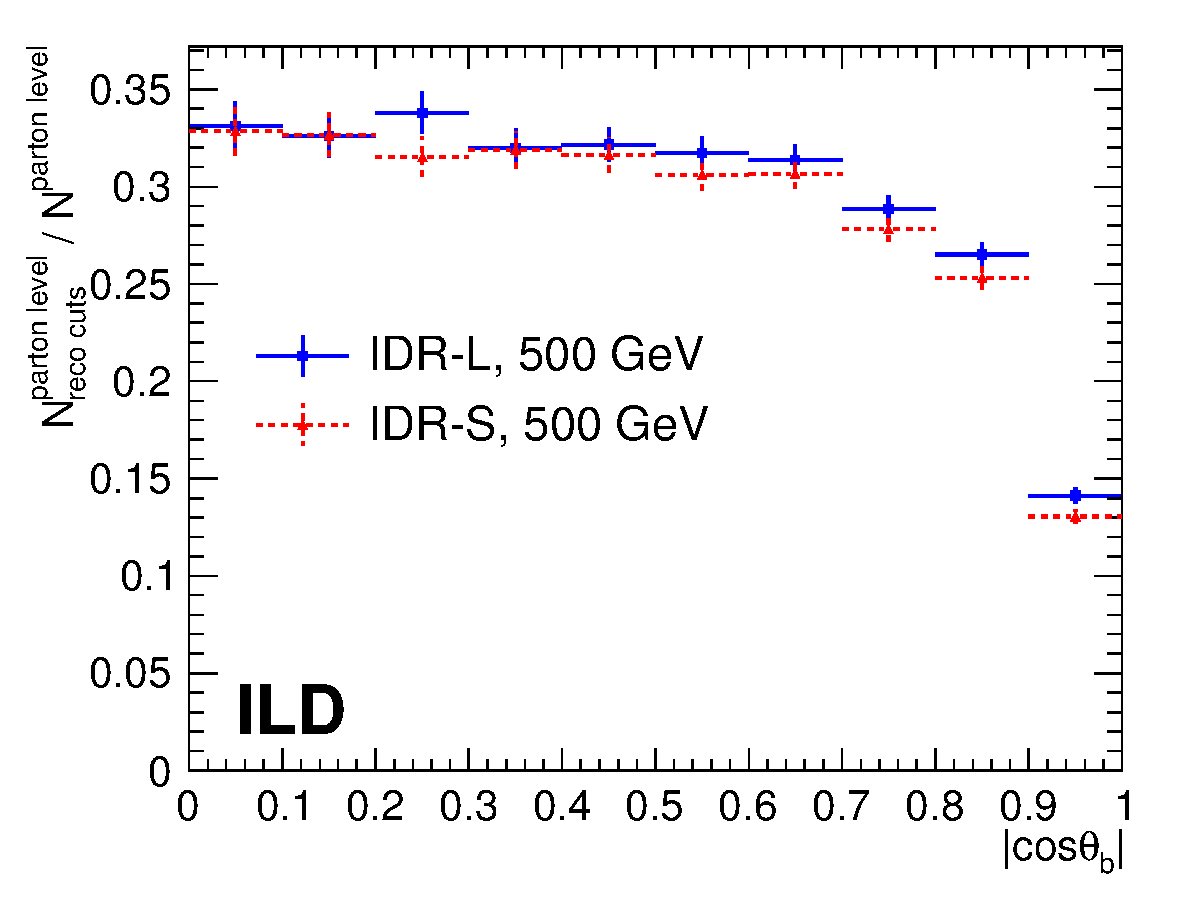
\includegraphics[width=\textwidth]{Performance/fig/acceptance_2models_v2.pdf}
 \caption{ \label{fig:bbbar:effipur:effi}}
 \end{subfigure}
%\hspace{0.03\textwidth}
\begin{subfigure}{0.49\hsize} 
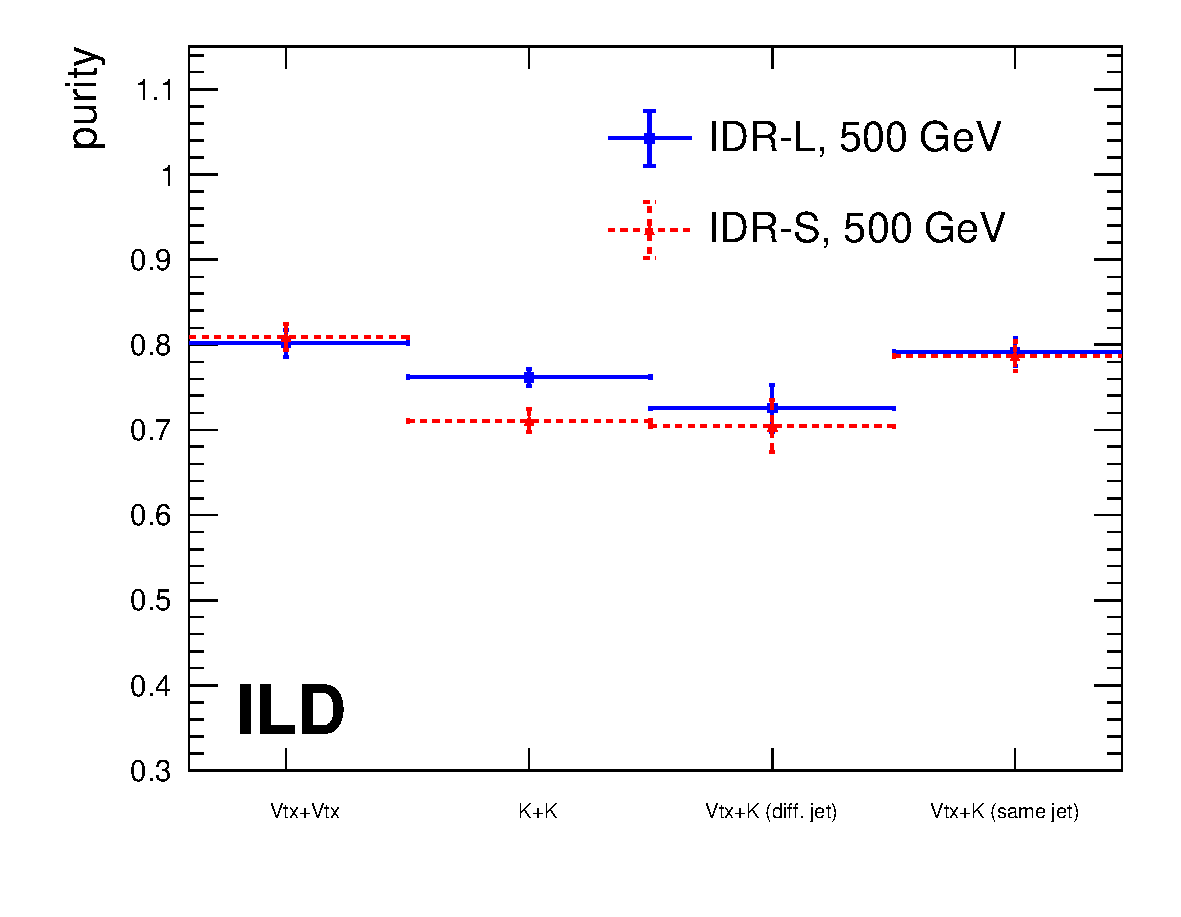
\includegraphics[width=\textwidth]{Performance/fig/purity_v3.pdf}
 \caption{  \label{fig:bbbar:effipur:pur}}
 \end{subfigure}
%\end{center}
\caption{
(a) Acceptance of the $e^+e^- \to b\bar{b}$ analysis as a function of $\cos{\theta}$ of the $b$-quark for IDR-L and IDR-S.
(b) Purity of the four different categories for charge tagging for IDR-L and IDR-S. 
}
\label{fig:bbbar:effipur}
\end{figure}

Figure~\ref{fig:bbbar:effipur:effi} compares the acceptance of the $b$-jet reconstruction for the large and the small version of ILD.
For $|\cos{\theta_b}|>0.5$, corresponding to a large part of the endcap 
region, the acceptance of IDR-L is about 1\% larger than for IDR-S. The purity of the four combinations of charge-ID is shown in Fig.~\ref{fig:bbbar:effipur:pur}. While the charge-ID via vertex charge performs identically for both detectors, the Kaon-charge ID yields a higher purity for IDR-L due to the larger radius of the TPC, which improves the $dE/dx$ resolution. 

The reconstructed  $|\cos{\theta_b}|$ distribution is shown in Fig.~\ref{fig:bbbar:result} for an integrated luminosity of $46$\,fb$^{-1}$ with purely left-handed electrons and right-handed positrons. The distributions obtained for both detectors are compared with the parton level. The results for both detector models agree within the statistical uncertainty given by the size of the simulated sample. However the migration from larger to smaller $\cos{\theta_b}$ seems to be larger in case of the small detector model.


\begin{figure}[htbp]
\begin{center} 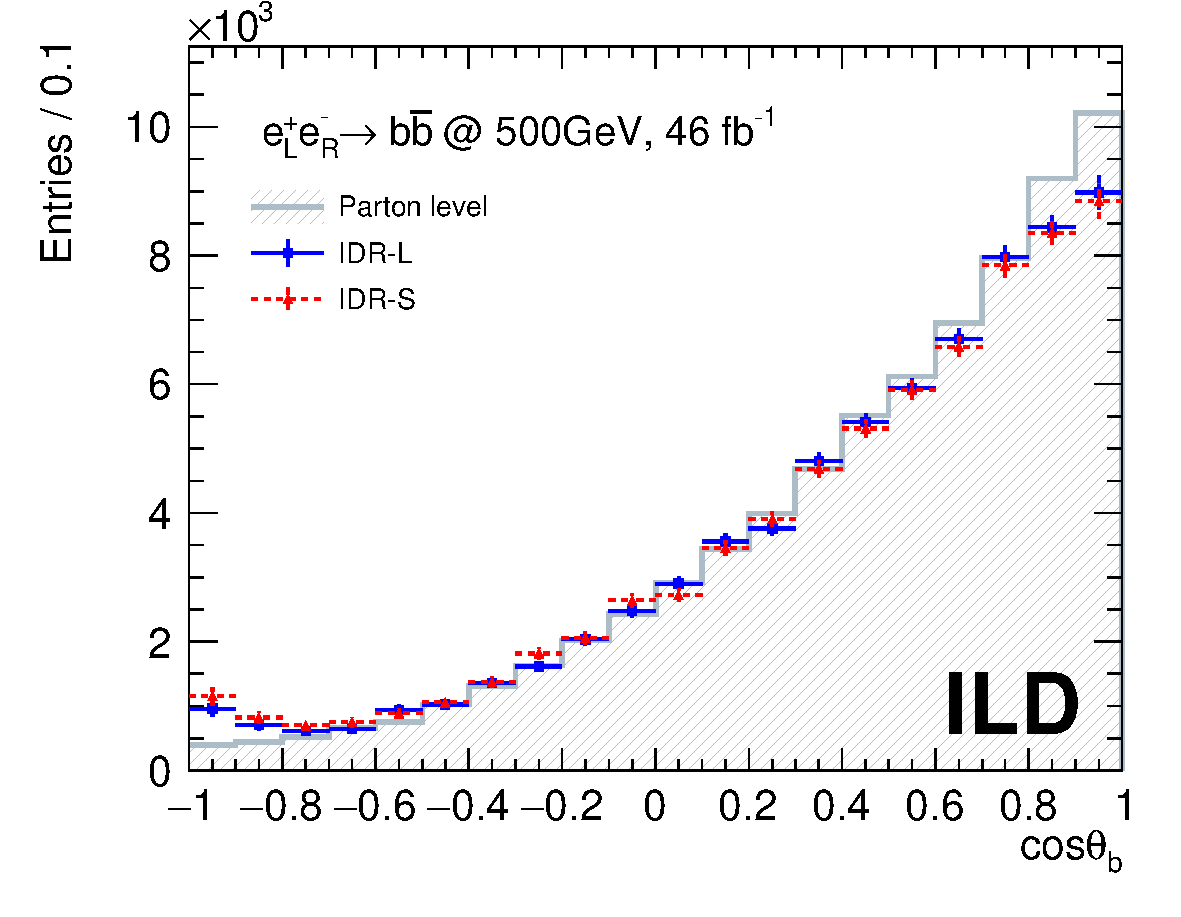
\includegraphics[width=0.55\textwidth]{Performance/fig/result2models_v3.pdf}
\end{center}
\caption{Generator-level distribution of $\cos{\theta_b}$ and the corresponding reconstructed distributions for IDR-L and IDR-S. The distribution is shown for a simulated sample of $46$\,fb$^{-1}$ for pure $e^-_L e^+_R$ beams.}
\label{fig:bbbar:result}
\end{figure}

%%%%%%%%%%%%%%%%%%%%%%%%%%%%%%%%%%%%%%%%%%%%%%%%%%%%%%%%%%%%%%%%%%%
\subsection{\texorpdfstring{$A_{FB}$ and polarised cross sections from $tt \to bb qql\nu$}{AFB and ALR from tt -> bbqqlv}}
\label{subsec:bench:ttbar}
%%%%%%%%%%%%%%%%%%%%%%%%%%%%%%%%%%%%%%%%%%%%%%%%%%%%%%%%%%%%%%%%%%%

The forward-backward asymmetry and the polarised cross sections of $e^+e^- \to t\bar{t}$ are crucial ingredients to the determination of the couplings of top quark to the photon and the $Z$ boson. In the semi-leptonic channel, which represents 43.5\% of all $t \bar t$ decays, the lepton charge is available to distiguish between the $t$ and the $\bar{t}$ quark. In the fully hadronic case, representing 46.5\% of all $t\bar t$ decays, $t$ and the $\bar{t}$ can only be distinguished by identifying the $b$ and $\bar{b}$-jets. For this purpose, the same techniques as presented in the previous subsection can be used, namely the charge at the secondary vertex and the charge of a Kaon in the jet (if present). While these techniques are common between the $e^+e^- \to b\bar{b}$ and $e^+e^- \to t\bar{t}$ cases, the two benchmarks probe very different momentum ranges for the Kaon as well as for the tracks forming the secondary vertex: The $b\bar{b}$ case offers a sample of back-to-back jets with typically $200-250$\,GeV each, while the $t\bar{t}$ case, the majority of the $b(\bar{b})$ jets have momenta of less than $50$\,GeV. Furthermore, the 6-fermion final state presents a much more busy environment than the 2-fermion final state.
Therefore, the two channels are complementary in terms of evaluating the detector performance. This is for instance reflected by the $5\%$ higher purity of the Kaon ID in case of the $t\bar{t}$ benchmark, c.f.\ Fig.~\ref{fig:perf:KaonID} in Sec.~\ref{sec:perf:sys:pid}.

As a $t\bar{t}$ benchmark for this document, the semi-leptonic channel was chosen, because it also tests the lepton (charge) reconstruction. Nevertheless, the Kaon and vertex charge tags can be applied on the $b(\bar{b})$-jets in addition. The inclusion of the The full description of the analysis can be found in~\cite{ILDNote:bbtt}. 

Like in the $e^+e^- \to b\bar{b}$ case, an event is considered only if two independent charge tags give consistent information. They can be from the lepton and one of the $b$-tagged jets (``K+L'', ``Vtx+L'') from both $b$-tagged jets (``K+K'', ``Vtx+Vtx'', ``Vtx+K'') or even from the same $b$-tagged jet (``Vtx+K$'$''). The purities of several double-tag combinations are compared for the large and small detector models in Fig.~\ref{fig:ttbar:effi}. While the size of the detector has no direct influence on the semi-leptonic analysis, especially the Kaon-ID based methods achieve a higher purity in case of the large detector. Overall, the combination of all the double-tag methods
increases the available statistics by about $40\%$ compared to using the lepton charge alone, from $22\%$ to $30\%$. 

\begin{figure}[htbp]
\begin{center} 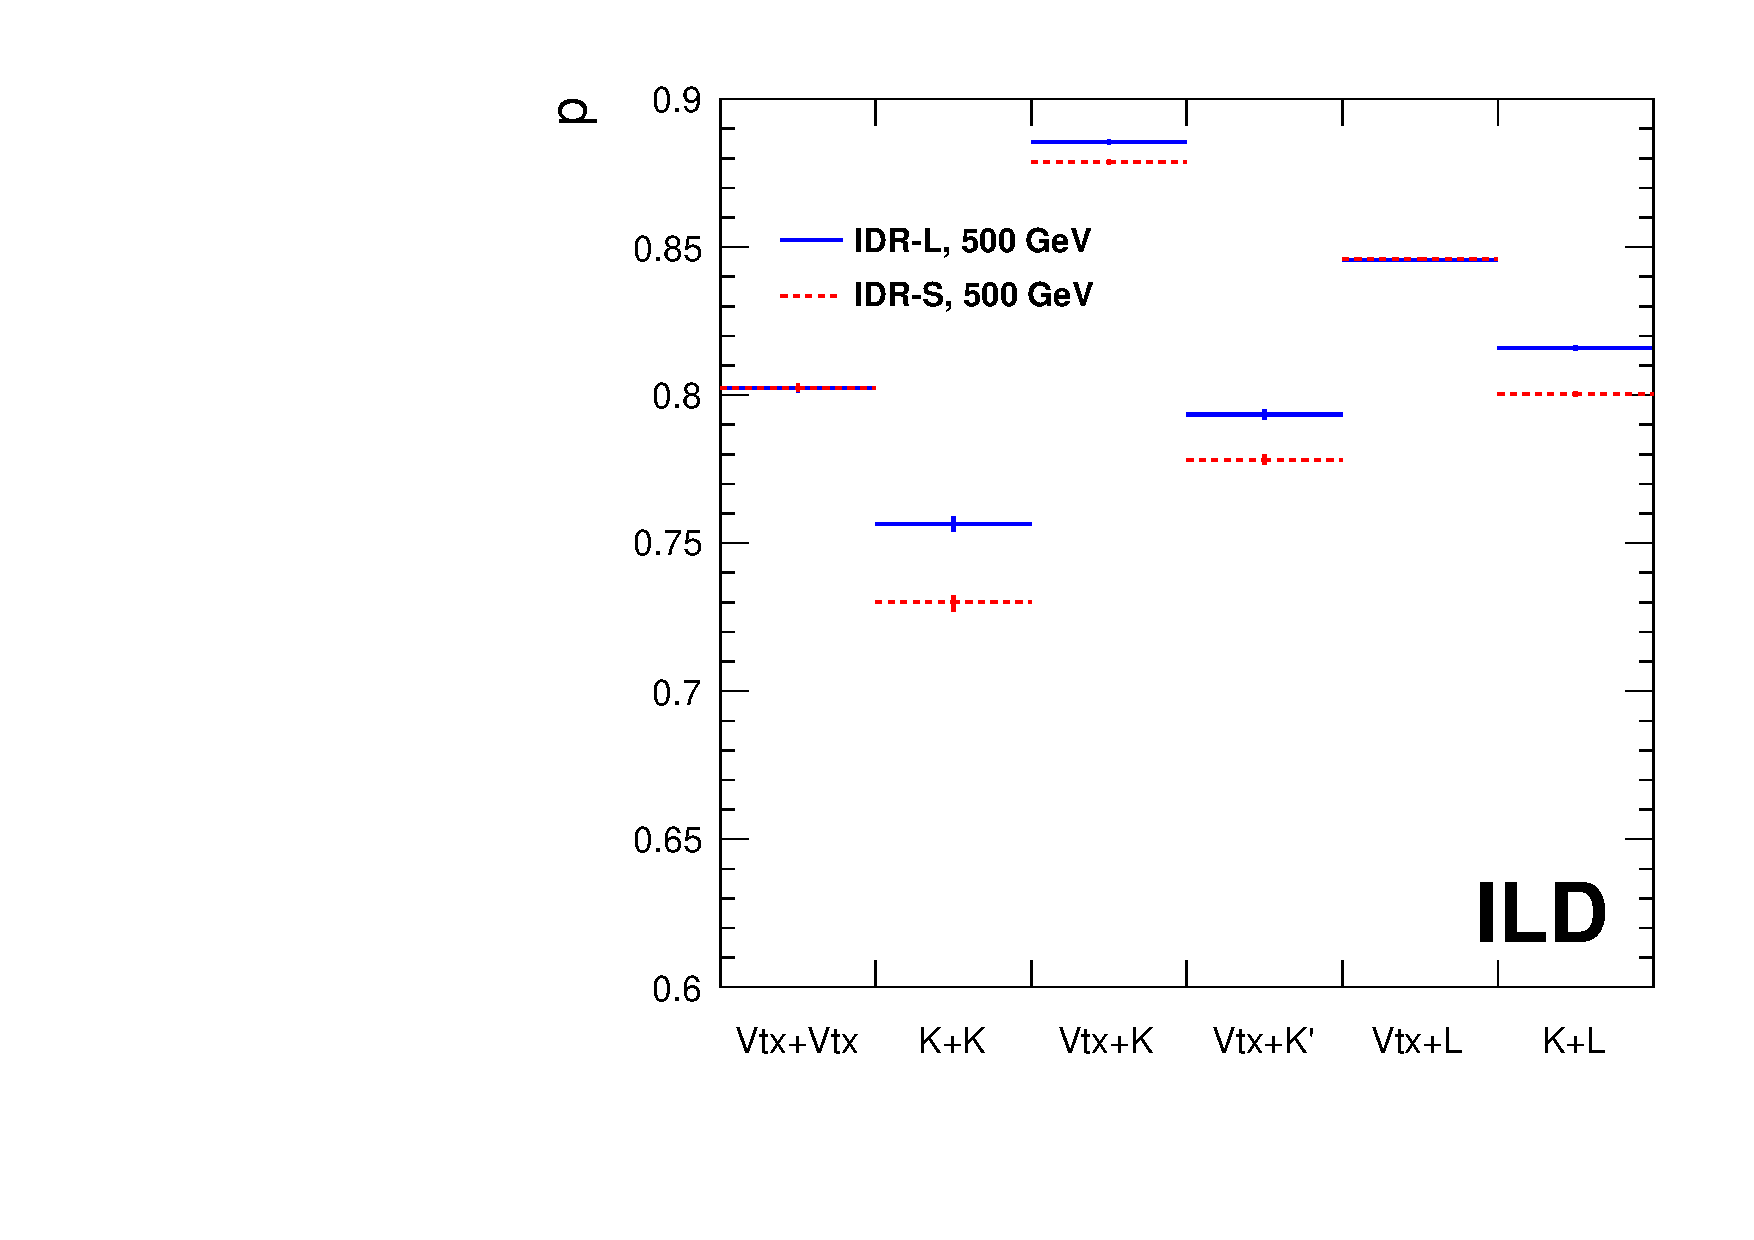
\includegraphics[width=0.55\textwidth]{Performance/fig/p_value_l5_ele_mu_noLcut.pdf}
\end{center}
\caption{Purity of the different double-tag methods to identify the charge of the $t$/$\bar{t}$ quarks. ``Vtx+K'' and `Vtx+K$'$'' refer to the vertex and Kaon charge tags in different jets and in the same jet, respectively. As expected, the double Kaon tag shows the largest difference between the two detector models due to the different TPC radius.}
\label{fig:ttbar:effi}
\end{figure}

If the lepton tag is (artificially) ignored, the channel is a perfect proxy for estimating the performance achievable in the fully hadronic channel. The jet-based double-tag methods alone yield an efficiency of about $15\%$. This means that from a future inclusion of the fully hadronic channel in the analysis a $50\%$ increase in the statistics available for the asymmetry and cross-section measurements.



\begin{figure}[htbp]
%\begin{center}
\begin{subfigure}{0.475\hsize} 
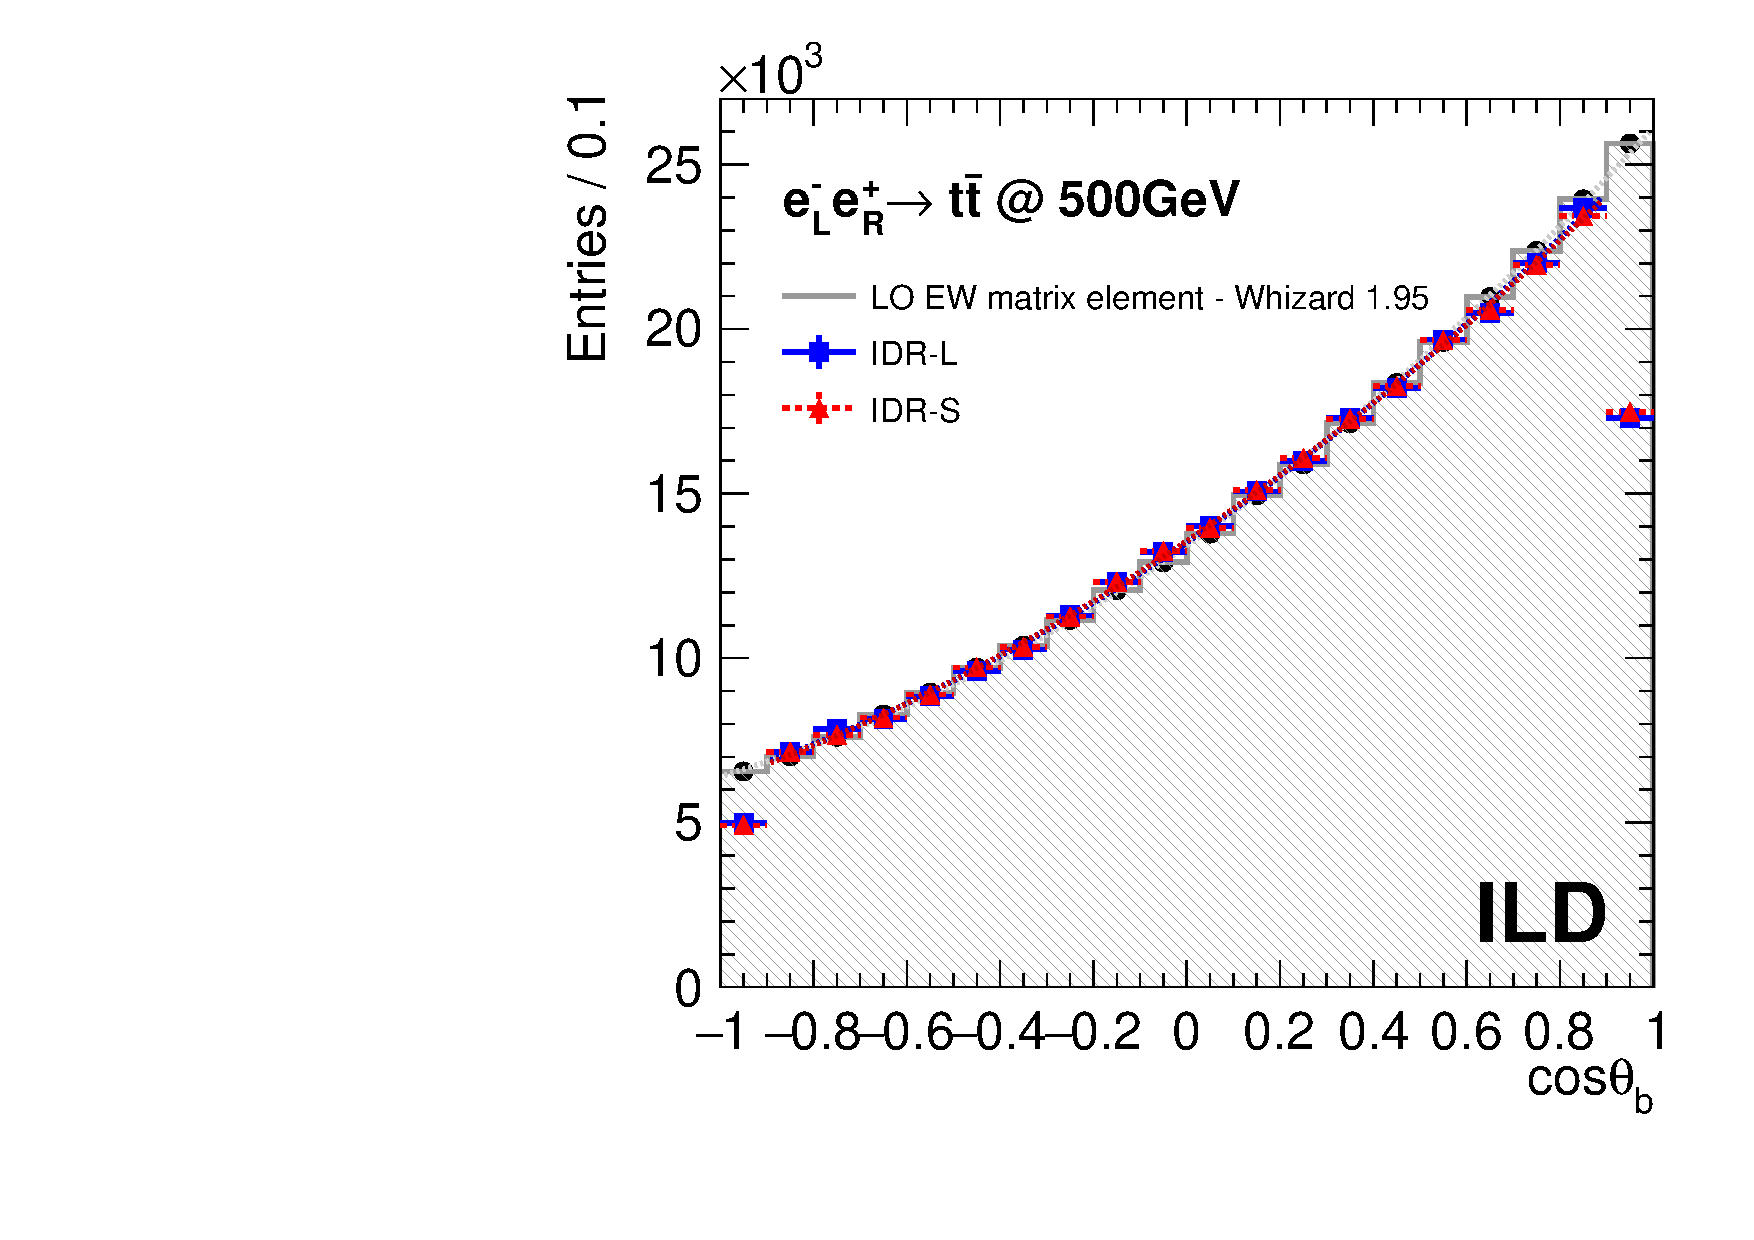
\includegraphics[width=\textwidth]{Performance/fig/compare_normalized_b.pdf}
 \caption{ \label{fig:ttbar:costhetab}}
 \end{subfigure}
%\hspace{0.03\textwidth}
\begin{subfigure}{0.475\hsize} 
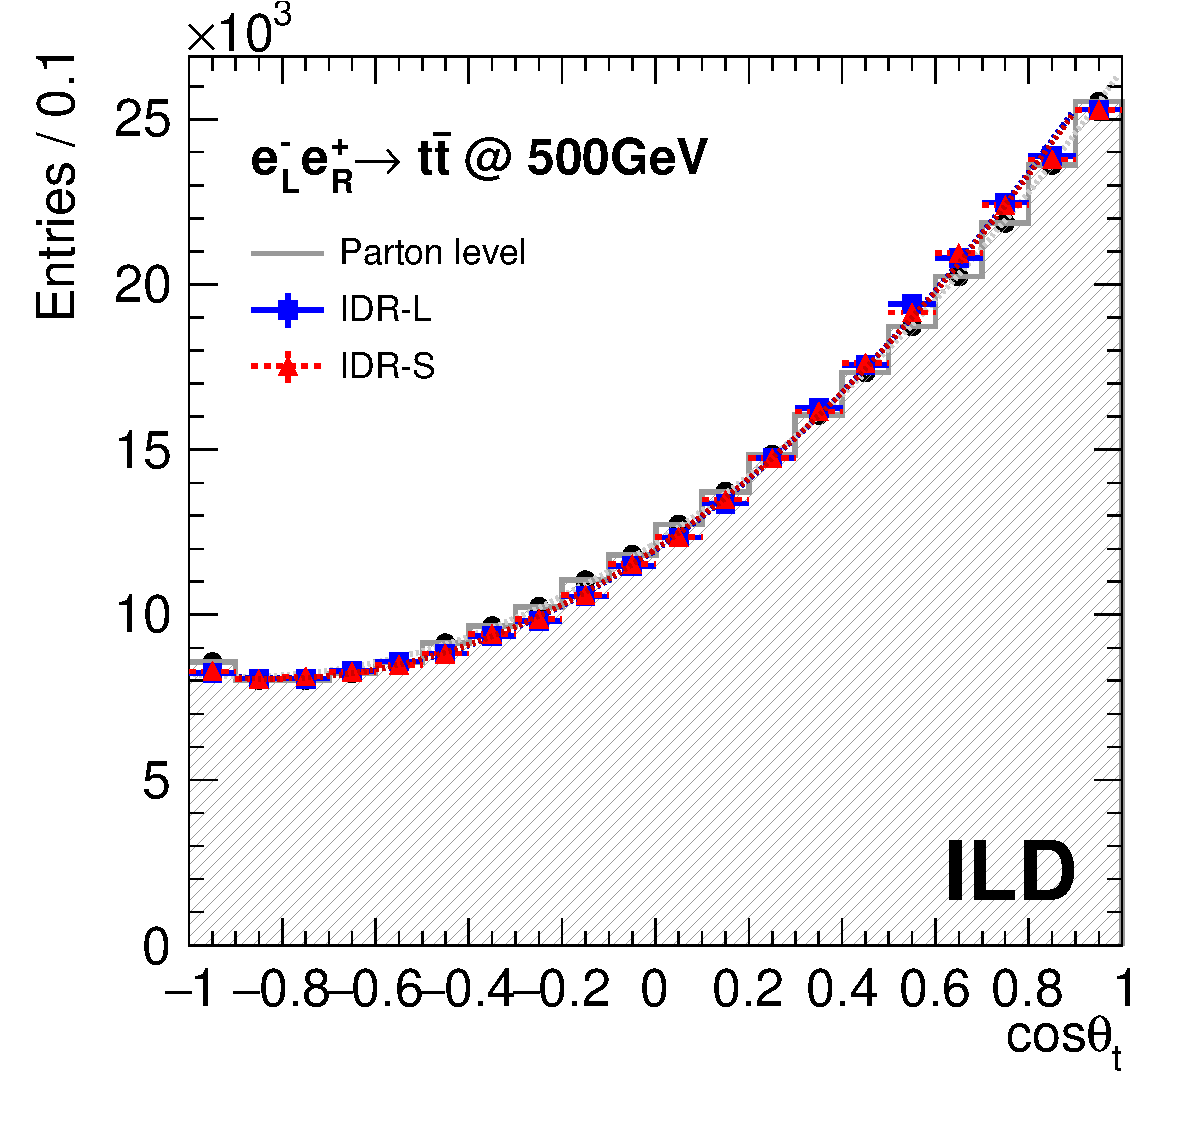
\includegraphics[width=\textwidth]{Performance/fig/compare_normalized.pdf}
 \caption{  \label{fig:ttbar:costhetat}}
 \end{subfigure}
%\end{center}
\caption{Polar angle distributions at leading order matrix element level and at reconstruction level for IDR-L and IDR-S. The distributions are shown for pure $e^-_L e^+_R$ data, in arbitrary absolute normalisation. Results corresponding to ILC500 as defined in  Sec.~\ref{sec:benchmarks:lep} are given in Tab.~\ref{tab:AFBtt}.
(a) Polar angle of the $b$-quark $\cos{\theta_b}$. 
(b) Polar angle of the $t$-quark $\cos{\theta_t}$.
}
\label{fig:ttbar:result}
\end{figure}

The reconstructed  polar angle ($\cos{\theta_t}$) distribution is shown for the purely left-handed electron and purely right-handed positron case in Fig.~\ref{fig:ttbar:costhetat}. Thereby, $\cos{\theta_t}$ is the polar angle of the three-momentum calculated from the two reconstructed tops as $\vec{p}_{t\bar{t}} = \vec{p}_t-\vec{p}_{\bar t}$. Figure~\ref{fig:ttbar:costhetab} shows the -- analoguously calculated -- polar angle spectrum of the $b$ quark that is emitted from the $t$ decay. This observable has been studied for the first time for the IDR and adds to the physics potential of ILD.  Both, the polar angle spectrum of the $t$ quark and of the $b$ quark,  as reconstructed with the two detector models under study are compared to the leading-order electroweak matrix element prediction. No difference is found here between the two detector models.
 
\begin{figure}[htbp]
%\begin{center}
\begin{subfigure}{0.475\hsize} 
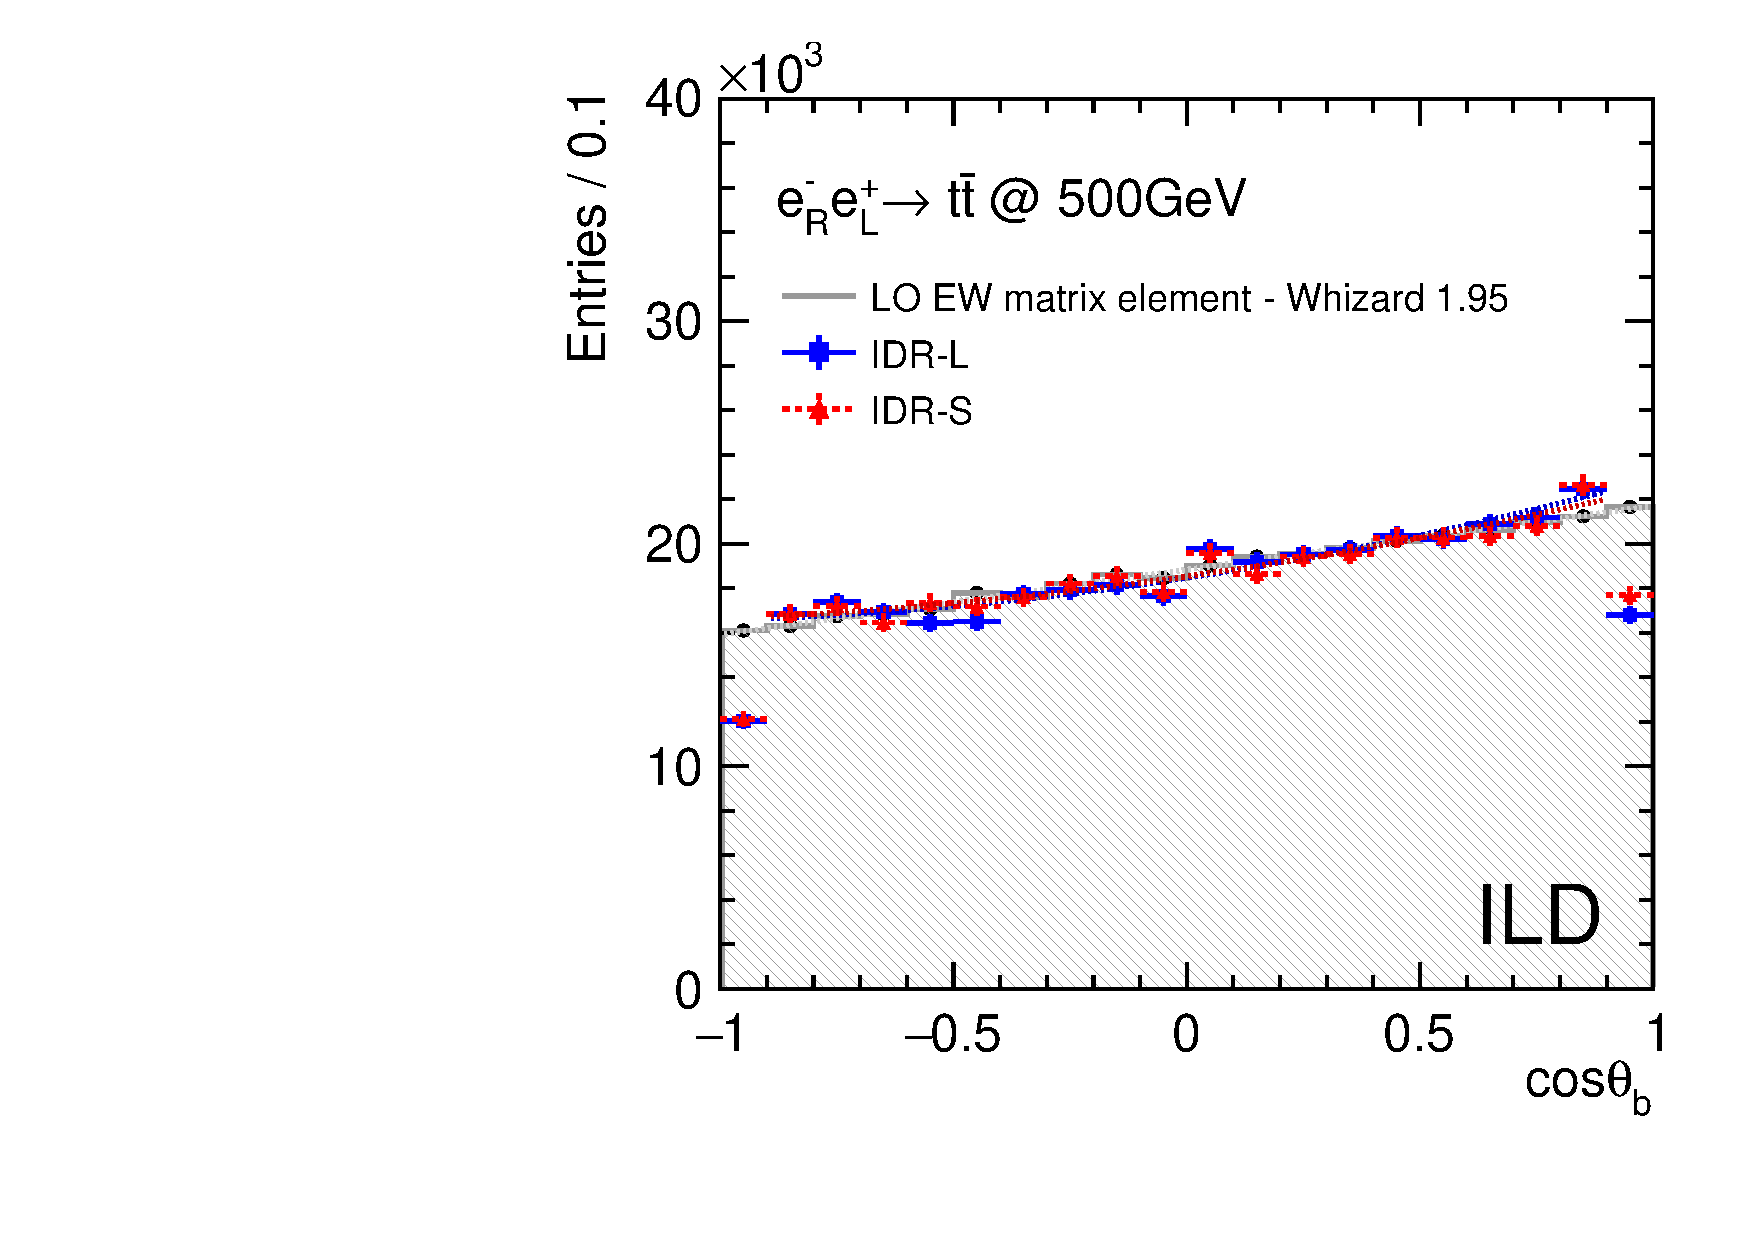
\includegraphics[width=\textwidth]{Performance/fig/compare_normalized_eRpL_b}
 \caption{ \label{fig:ttbar:costhetabRL}}
 \end{subfigure}
%\hspace{0.03\textwidth}
\begin{subfigure}{0.475\hsize} 
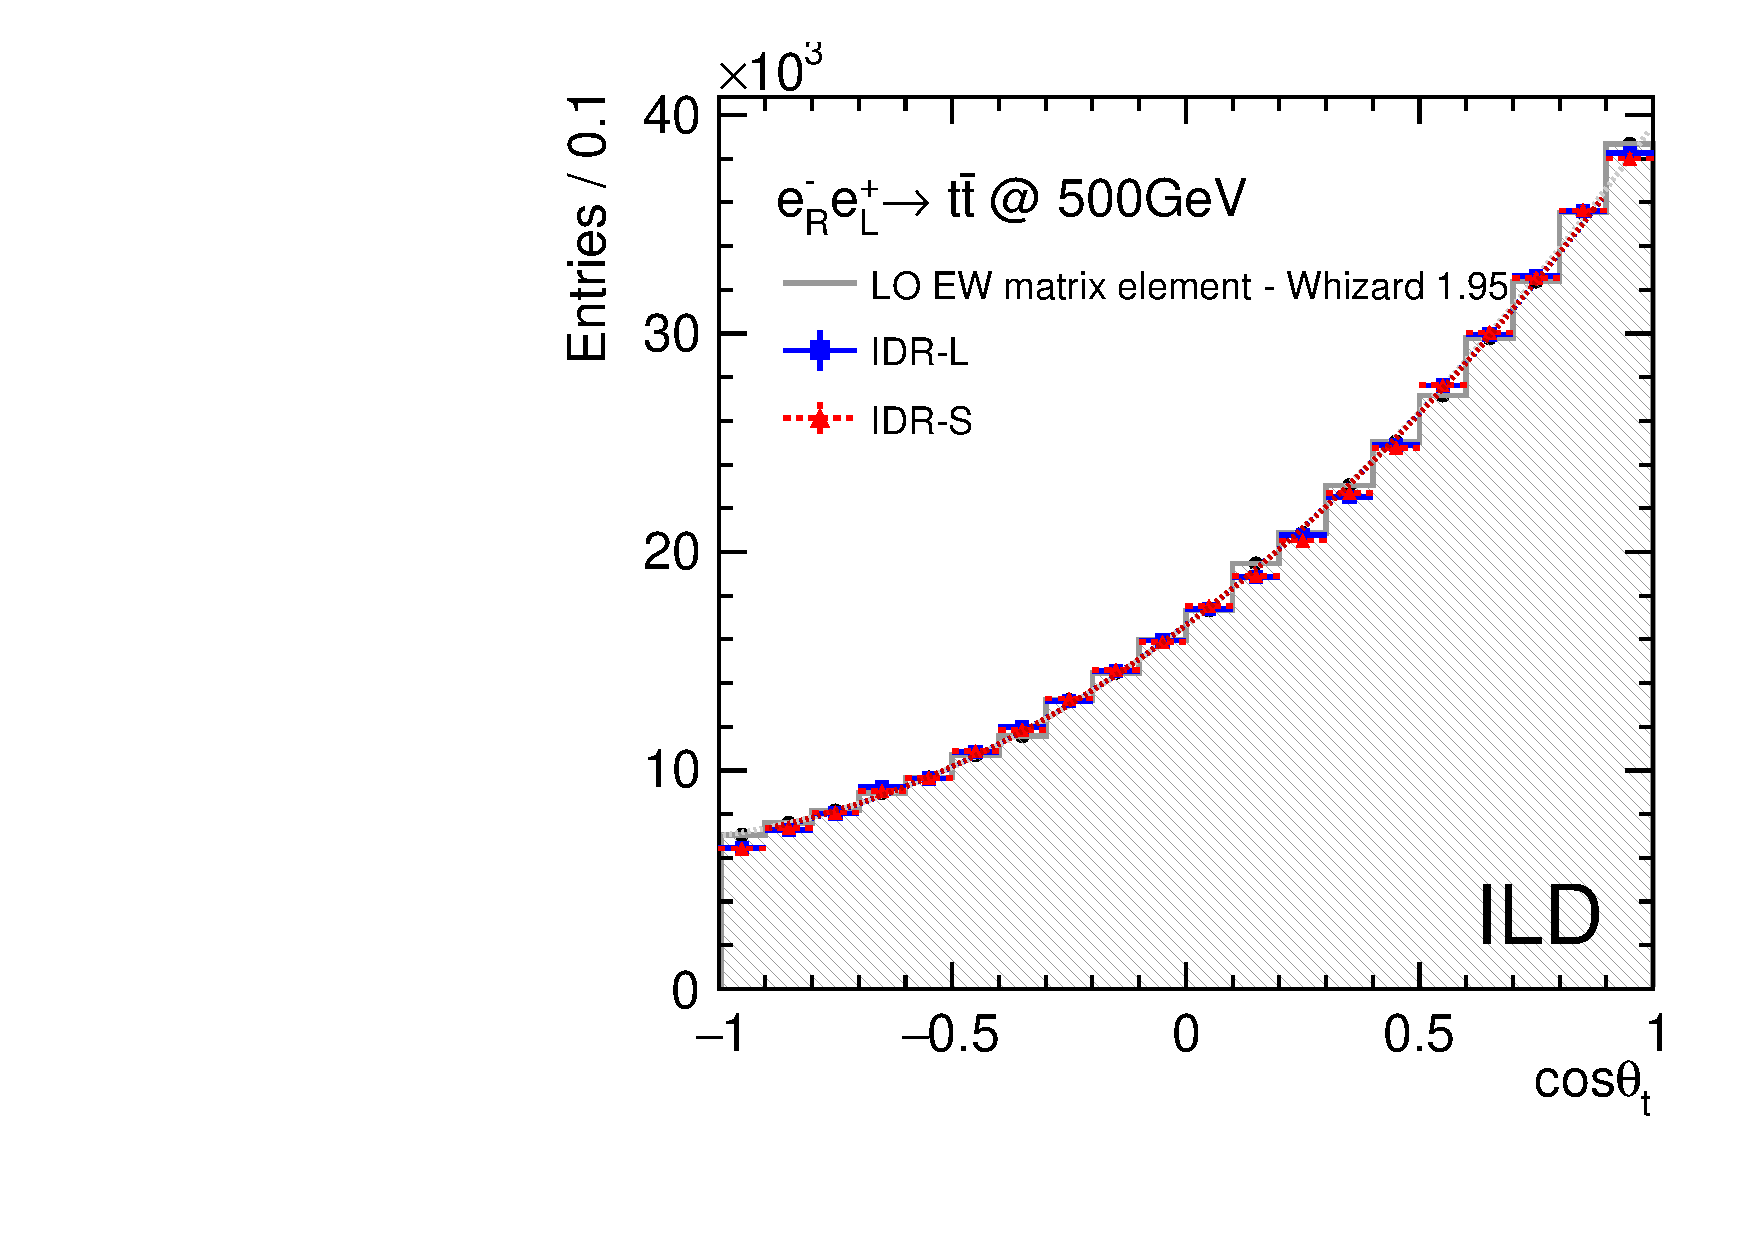
\includegraphics[width=\textwidth]{Performance/fig/compare_normalized_eRpL}
 \caption{  \label{fig:ttbar:costhetatRL}}
 \end{subfigure}
%\end{center}
\caption{Polar angle distributions at leading order matrix element level and at reconstruction level for IDR-L and IDR-S. The distributions are shown for pure $e^-_R e^+_L$ data, in arbitrary absolute normalisation. Results corresponding to ILC500 as defined in  Sec.~\ref{sec:benchmarks:lep} are given in Tab.~\ref{tab:AFBtt}.
(a) Polar angle of the $b$-quark $\cos{\theta_b}$. 
(b) Polar angle of the $t$-quark $\cos{\theta_t}$.
}
\label{fig:ttbar:resultRL}
\end{figure}

The analogous distributions are shown in Fig.~\ref{fig:ttbar:resultRL} for the opposite beam helicity configuration, again compared to the leading-order electroweak matrix element level. Also here, no difference is found here between the two detector models.  Note the difference in the polar angle spectra of the $b$ quark between Figs.~\ref{fig:ttbar:costhetab}, and~\ref{fig:ttbar:costhetabRL} which is due to the $V-A$ interaction at the $tbW$ vertex.

The resulting precisions on the polarised cross sections as well as on $A_{FB}$ as expected for the $P(e^-,e^+)=(\pm 80\%, \mp 30\%)$ data sets of ILC500 as defined in Sec.~\ref{sec:benchmarks:lep} are equal for the two detector models as given in Tab.~\ref{tab:AFBtt}.

\begin{table}[htb]
\begin{center}
\begin{tabular}{|c|c|c|c|}
\hline
 & $P(e^-,e^+)$ & $(\delta\sigma / \sigma)_{stat} [\%]$ & $(\delta A_{FB}^t / A_FB^t)_{stat} [\%]$ \\
\hline
\multirow{2}{*}{IDR-L/S} &  $(-80\%,+30\%)$ & 0.17 & 0.7 \\
                         &  $(+80\%,-30\%)$ & 0.25 & 0.53 \\
\hline
\end{tabular}
\end{center}
\caption{Statistical uncertainties on the polarised cross section and the top forward-backward asymmetry obtained in this analysis for the ILC500 as defined in Sec.~\ref{sec:benchmarks:lep}.}
\label{tab:AFBtt}   
\end{table}    

In order to put these results into perspective, they have been translated into $1\sigma$ precisions on the electromagnetic form factors of the top quark. These are displayed in Fig.~\ref{fig:ttbar:formfac} in comparison to the most recent projections for HL-LHC. %and estimates for FCCee~\cite{Janot:2015yza}. 
The projections for HL-LHC are derived from the {\em individual} constraints of EFT Wilson coefficients presented in Tab.\,C2.3 of Ref.~\cite{Durieux:2019rbz} (the most favorable scenario for HL-LHC). This figure clearly demonstrates the superiority of a linear $e^+e^-$ collider with polarised beams operated at an adequate center-of-mass energy.             
\begin{figure}[htbp]
\begin{center} 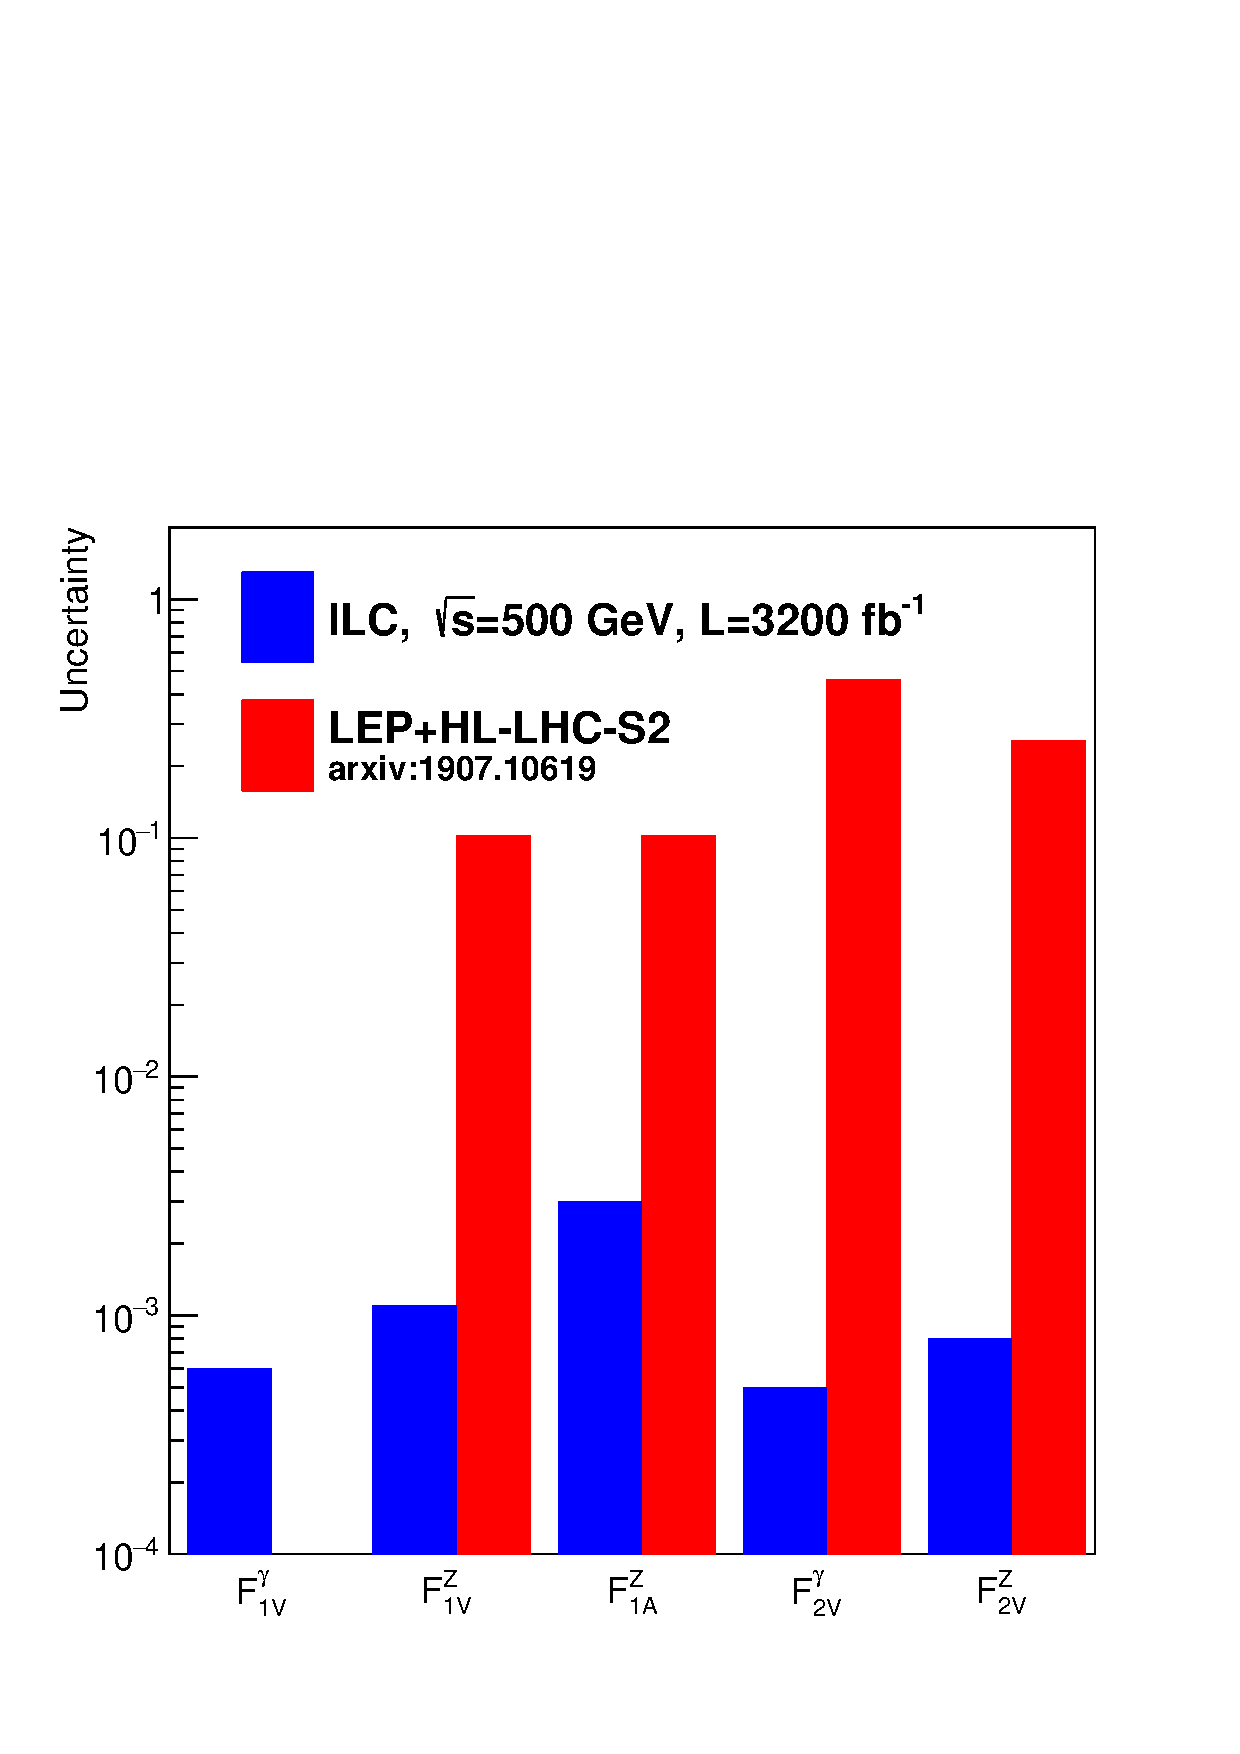
\includegraphics[width=0.6\textwidth]{Performance/fig/couplilclhc}
\end{center}
\caption{Expected precision on electromagnetic form factors of the top quark from this study, based on ILC500 as defined in Sec.~\ref{sec:benchmarks:lep}, compared to recent projections for the HL-LHC~\cite{Durieux:2019rbz}.}
\label{fig:ttbar:formfac}
\end{figure}

%%%%%%%%%%%%%%%%%%%%%%%%%%%%%%%%%%%%%%%%%%%%%%%%%%%%%%%%%%%%%%%%%%%
\subsection{Search for extra Scalars in \texorpdfstring{$e^+e^- \to ZS^0$}{e+e- -> ZS^0}}
\label{subsec:bench:extraH}
%%%%%%%%%%%%%%%%%%%%%%%%%%%%%%%%%%%%%%%%%%%%%%%%%%%%%%%%%%%%%%%%%%%

Searches for additional Higgs bosons or other new scalar particles, denoted here generically with $S^0$, are theoretically well-motivated, and benefit from an $e^+e^-$ collider sensitivity highly
complementary to that of hadron colliders. Due to the SM-likeness of the $125$-GeV Higgs boson, additional Higgs-like scalars are expected to have a suppressed coupling to the $Z$ boson. Nevertheless, they can 
be searched for using the same recoil technique which is the basis of the decay-mode independent measurement
of the total Higgsstrahlungs cross section. While in principle all visible decay modes of the $Z$ boson can
be exploited in this search, $Z\to\mu^+\mu^-$ as the cleanest mode has been chosen as a benchmark here~\cite{ILDNote:extraH}.
The two most important detector performance aspects for this analysis are the momentum resolution for the two
muons and the ability to detect and identify ISR photons in the detector. The latter applies in particular for the lower Higgs masses, where $M_{S^0} + M_Z << \sqrt{s}$ and thus significant photon radiation occurs frequently.
If the photon is detected, then the event kinematics can be corrected accordingly, which improves the separation of signal and background significantly.


\begin{figure}[htbp]
%\begin{center}
\begin{subfigure}{0.475\hsize} 
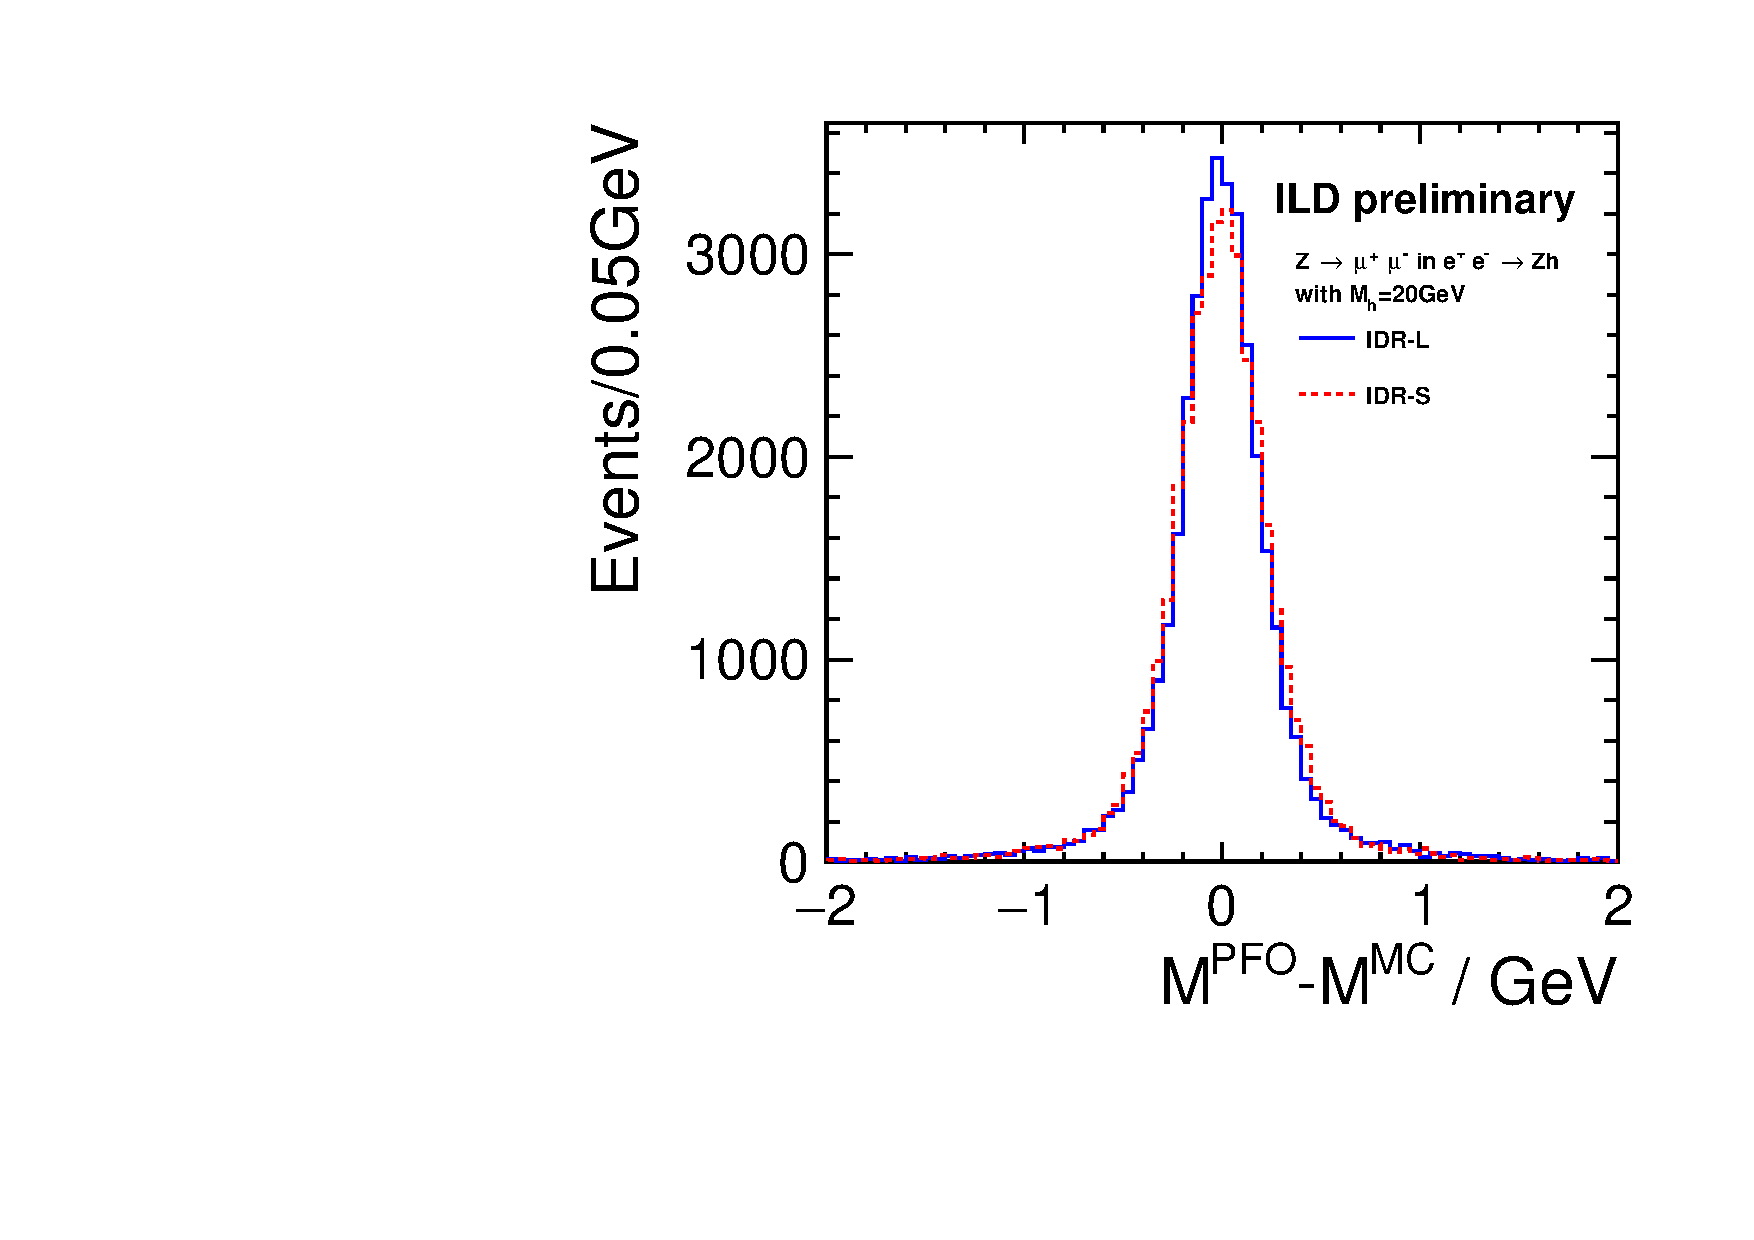
\includegraphics[width=\textwidth]{Performance/fig/lepton_pair_inm_difference_nh20.pdf}
 \caption{ \label{fig:extraH:Mdiff:mh20}}
 \end{subfigure}
%\hspace{0.03\textwidth}
\begin{subfigure}{0.475\hsize} 
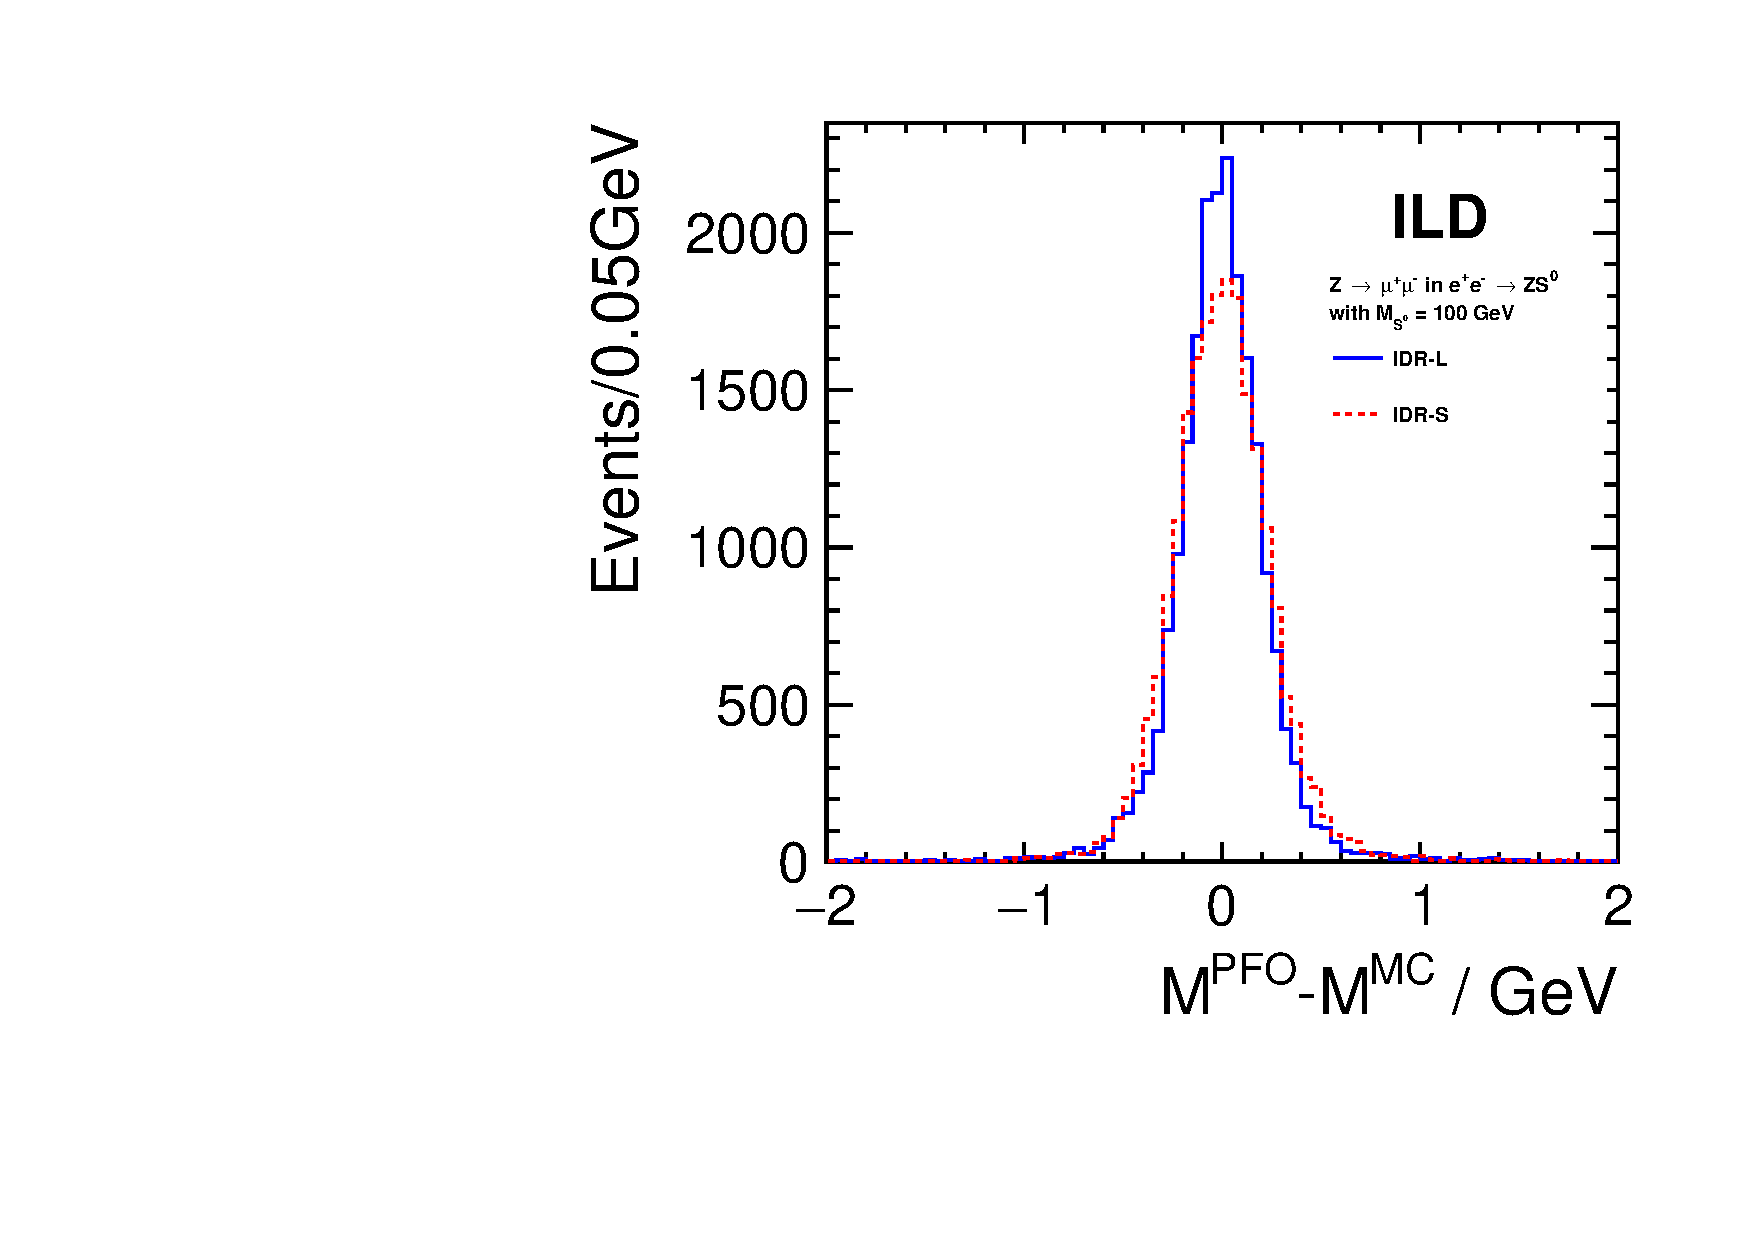
\includegraphics[width=\textwidth]{Performance/fig/lepton_pair_inm_difference_nh100.pdf}
 \caption{  \label{fig:extraH:Mdiff:mh100}}
 \end{subfigure}
\begin{subfigure}{0.475\hsize} 
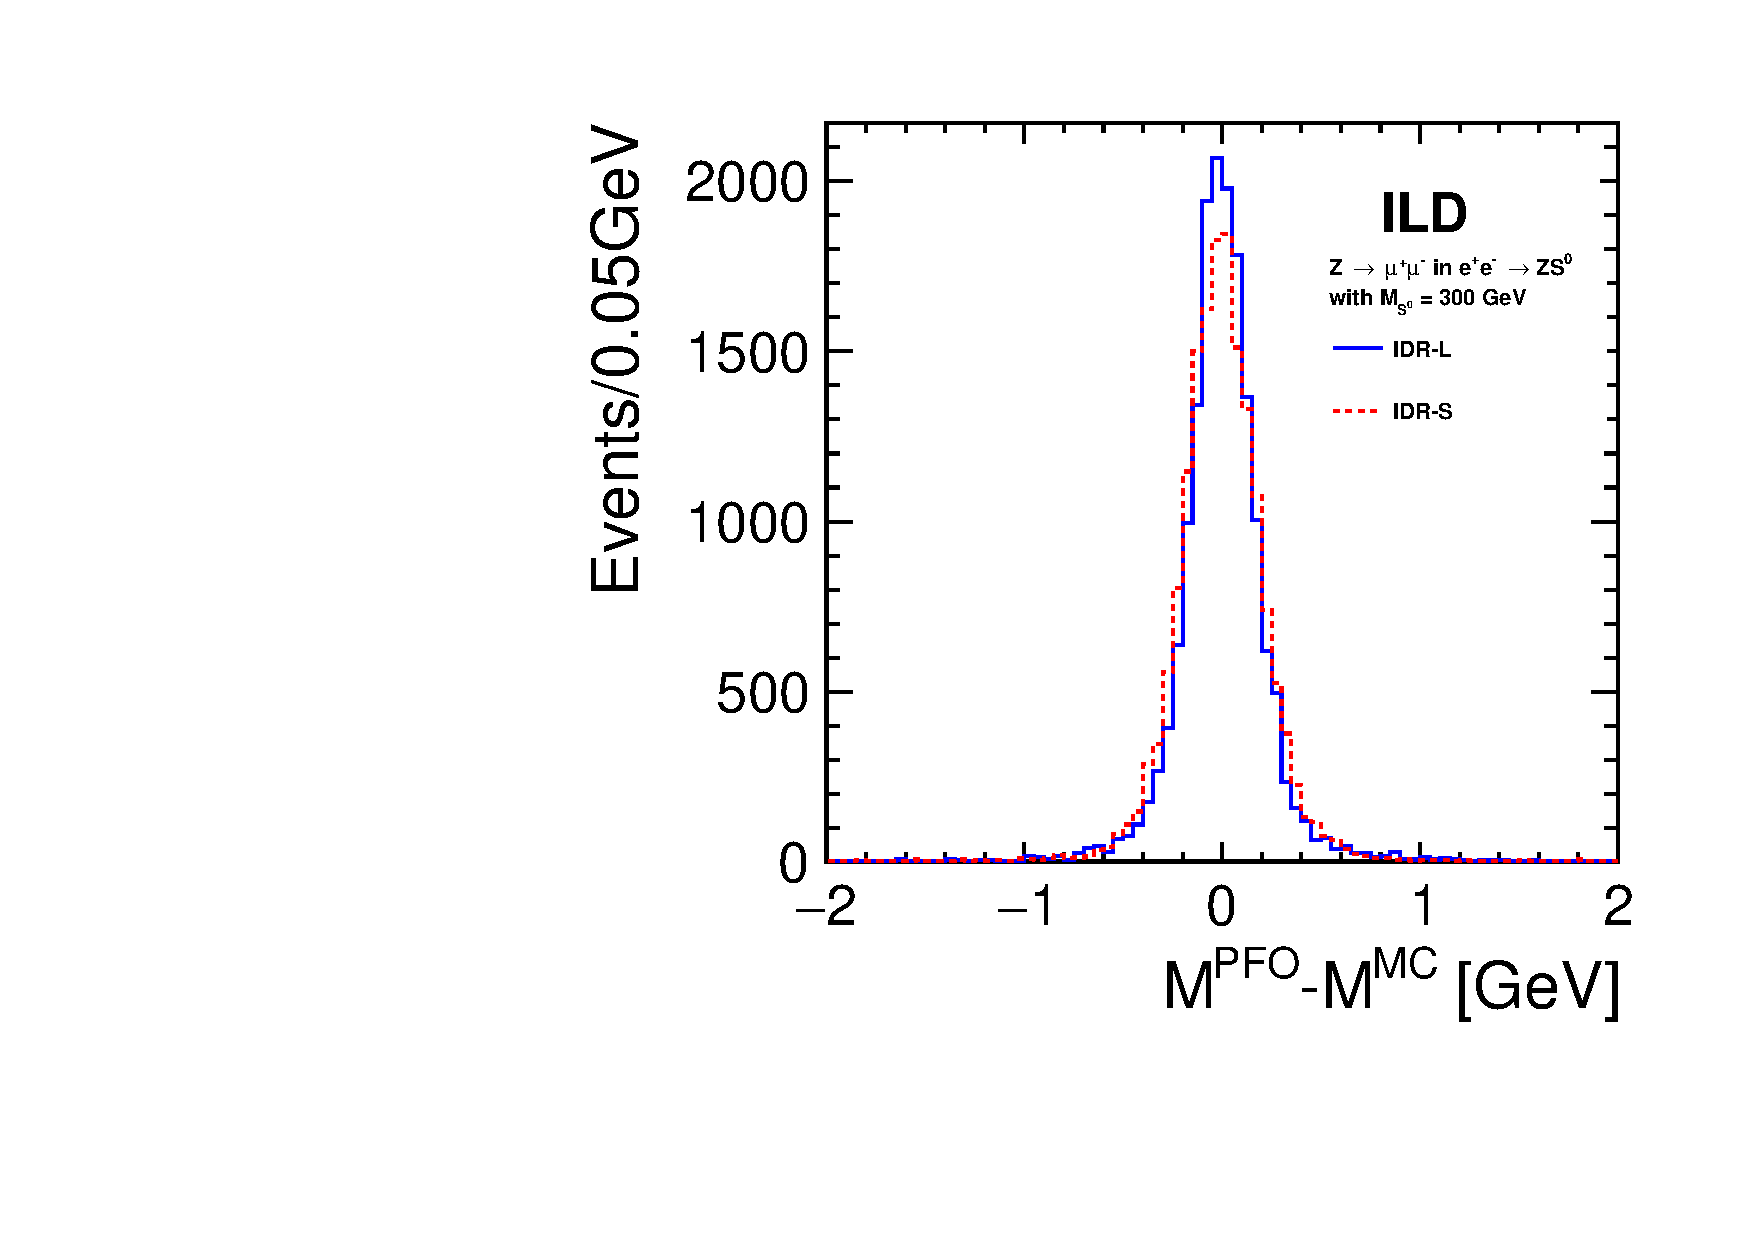
\includegraphics[width=\textwidth]{Performance/fig/lepton_pair_inm_difference_nh300.pdf}
 \caption{ \label{fig:extraH:Mdiff:mh300}}
 \end{subfigure}
%\hspace{0.03\textwidth}
\begin{subfigure}{0.475\hsize} 
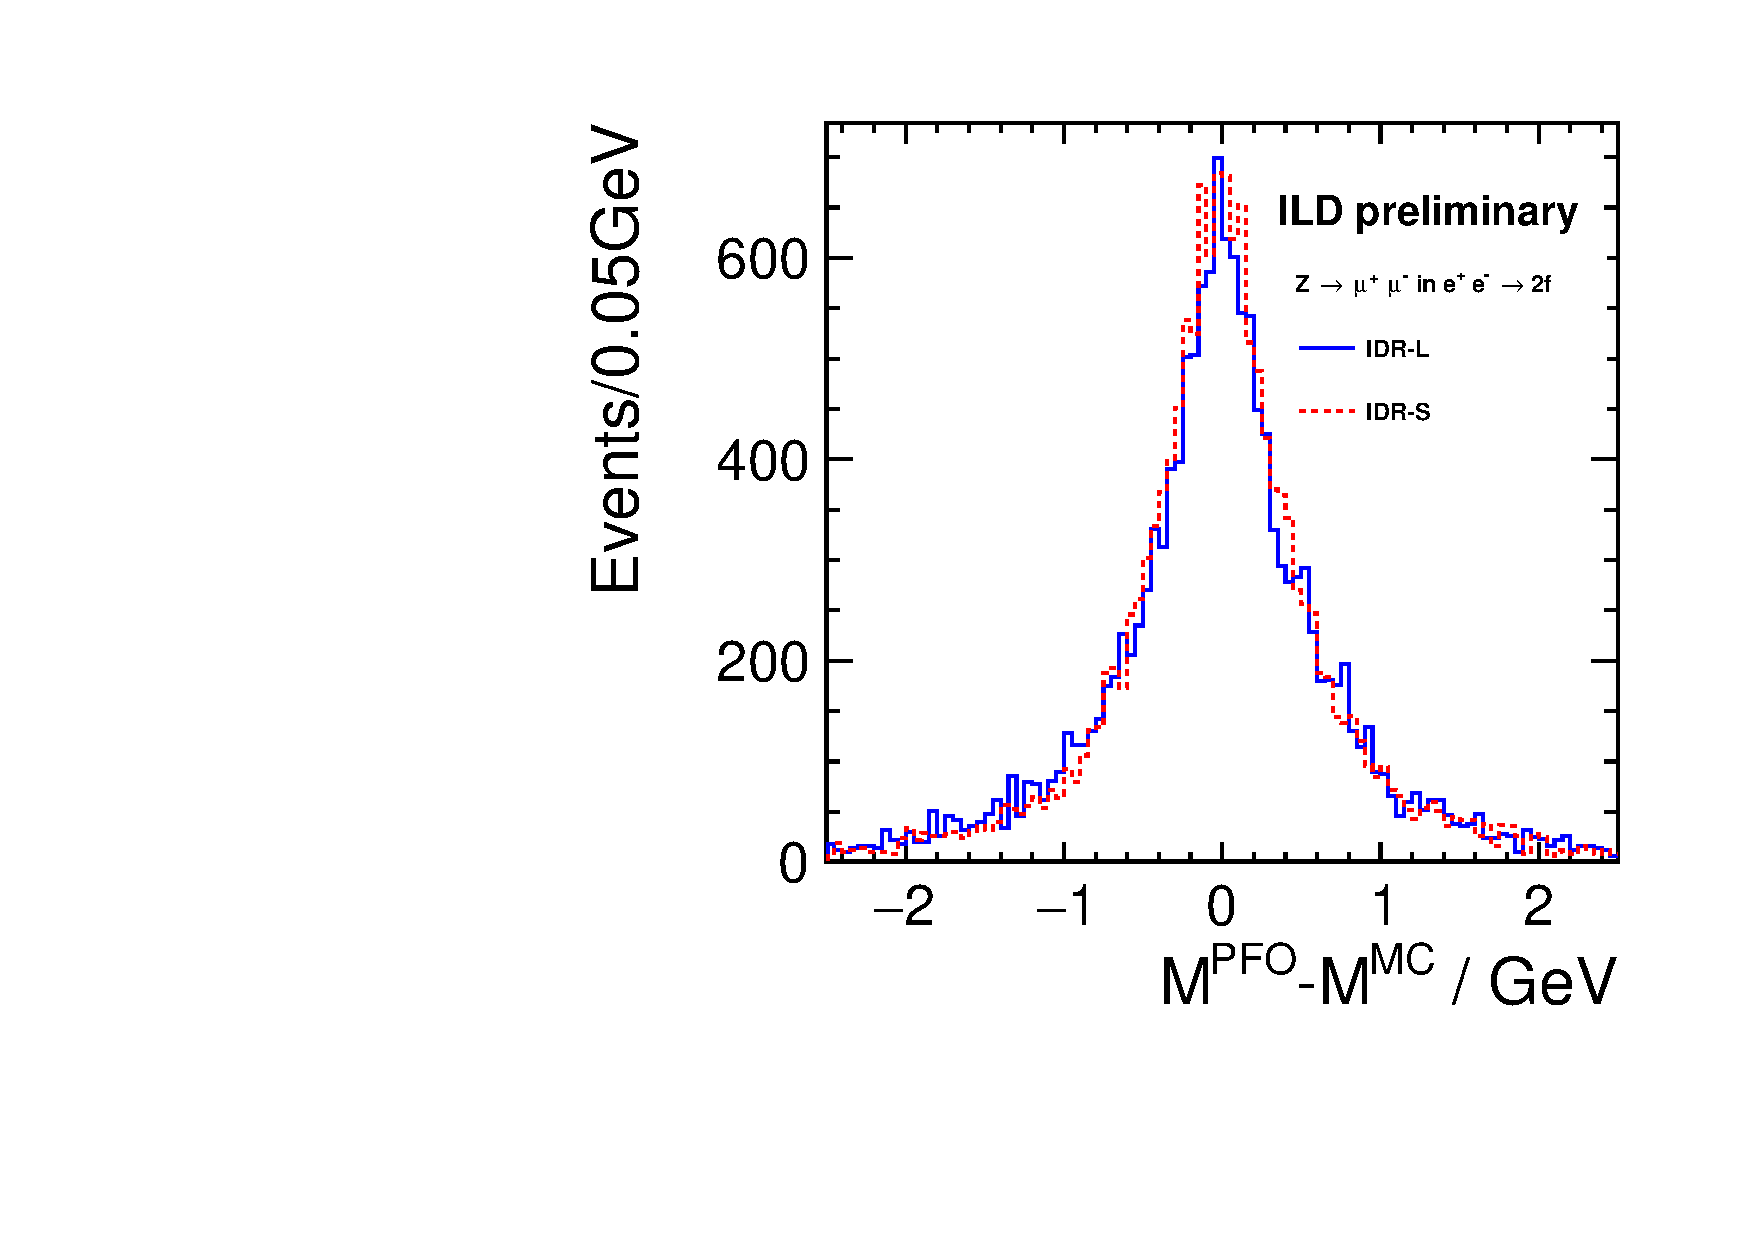
\includegraphics[width=\textwidth]{Performance/fig/lepton_pair_inm_difference_2f.pdf}
 \caption{  \label{fig:extraH:Mdiff:2f}}
 \end{subfigure}
%\end{center}
\caption{Event-by-event difference between reconstructed and generated di-muon mass for different types of events sampling different ranges in polar angle and momentum of the muons  in IDR-L and IDR-S:
(a) $ZS^0$ signal with $M_{S^0} = 20$\,GeV
(b) $ZS^0$ signal with $M_{S^0} = 100$\,GeV
(c) $ZS^0$ signal with $M_{S^0} = 300$\,GeV
(d) $2f$ background.
}
\label{fig:extraH:Mdiff}
\end{figure}

Figure~\ref{fig:extraH:Mdiff} shows the event-by-event difference between the reconstructed and generated di-muon mass for signal events with different scalar masses as well as for the 2-fermion background. The underlying distributions of momentum and polar angle differ significantly between the various samples. Therefore also the impact of the choice of detector model varies from sample to sample: With higher scalar masses, the $Z$ is less and less boosted, thus the muons are more and more central and back-to-back, resulting in an overall better mass reconstruction and a better performance of the large detector. In case of the $2$-fermion background, about half of the events return to the $Z$ pole, resulting in forward boosted $Z$'s with a small opening angle between the also forward-going muons. In those events which do not return to the $Z$, the muons have higher momenta than in the
signal samples. In combination, the mass reconstruction in the $2$-fermion events is worse, but when comparing
the two detector models, the better momentum resolution of ILD-S in the forward region and its worse resolution
in the barrel roughly cancel.




This can be seen much more clearly from the event-by-event mass uncertainty as calculated from the errors on 
the track parameters, shown in Fig~\ref{fig:extraH:Msigma} for the same four event samples. In case of the scalar
signal, the large detector always gives a significantly better resolution. In case of the $2$-fermion background, there is a small population at the smallest uncertainties which behaves like the signal, while for cases of the larger uncertainty, the small detector performs better than the large detector.

\begin{figure}[htbp]
%\begin{center}
\begin{subfigure}{0.475\hsize} 
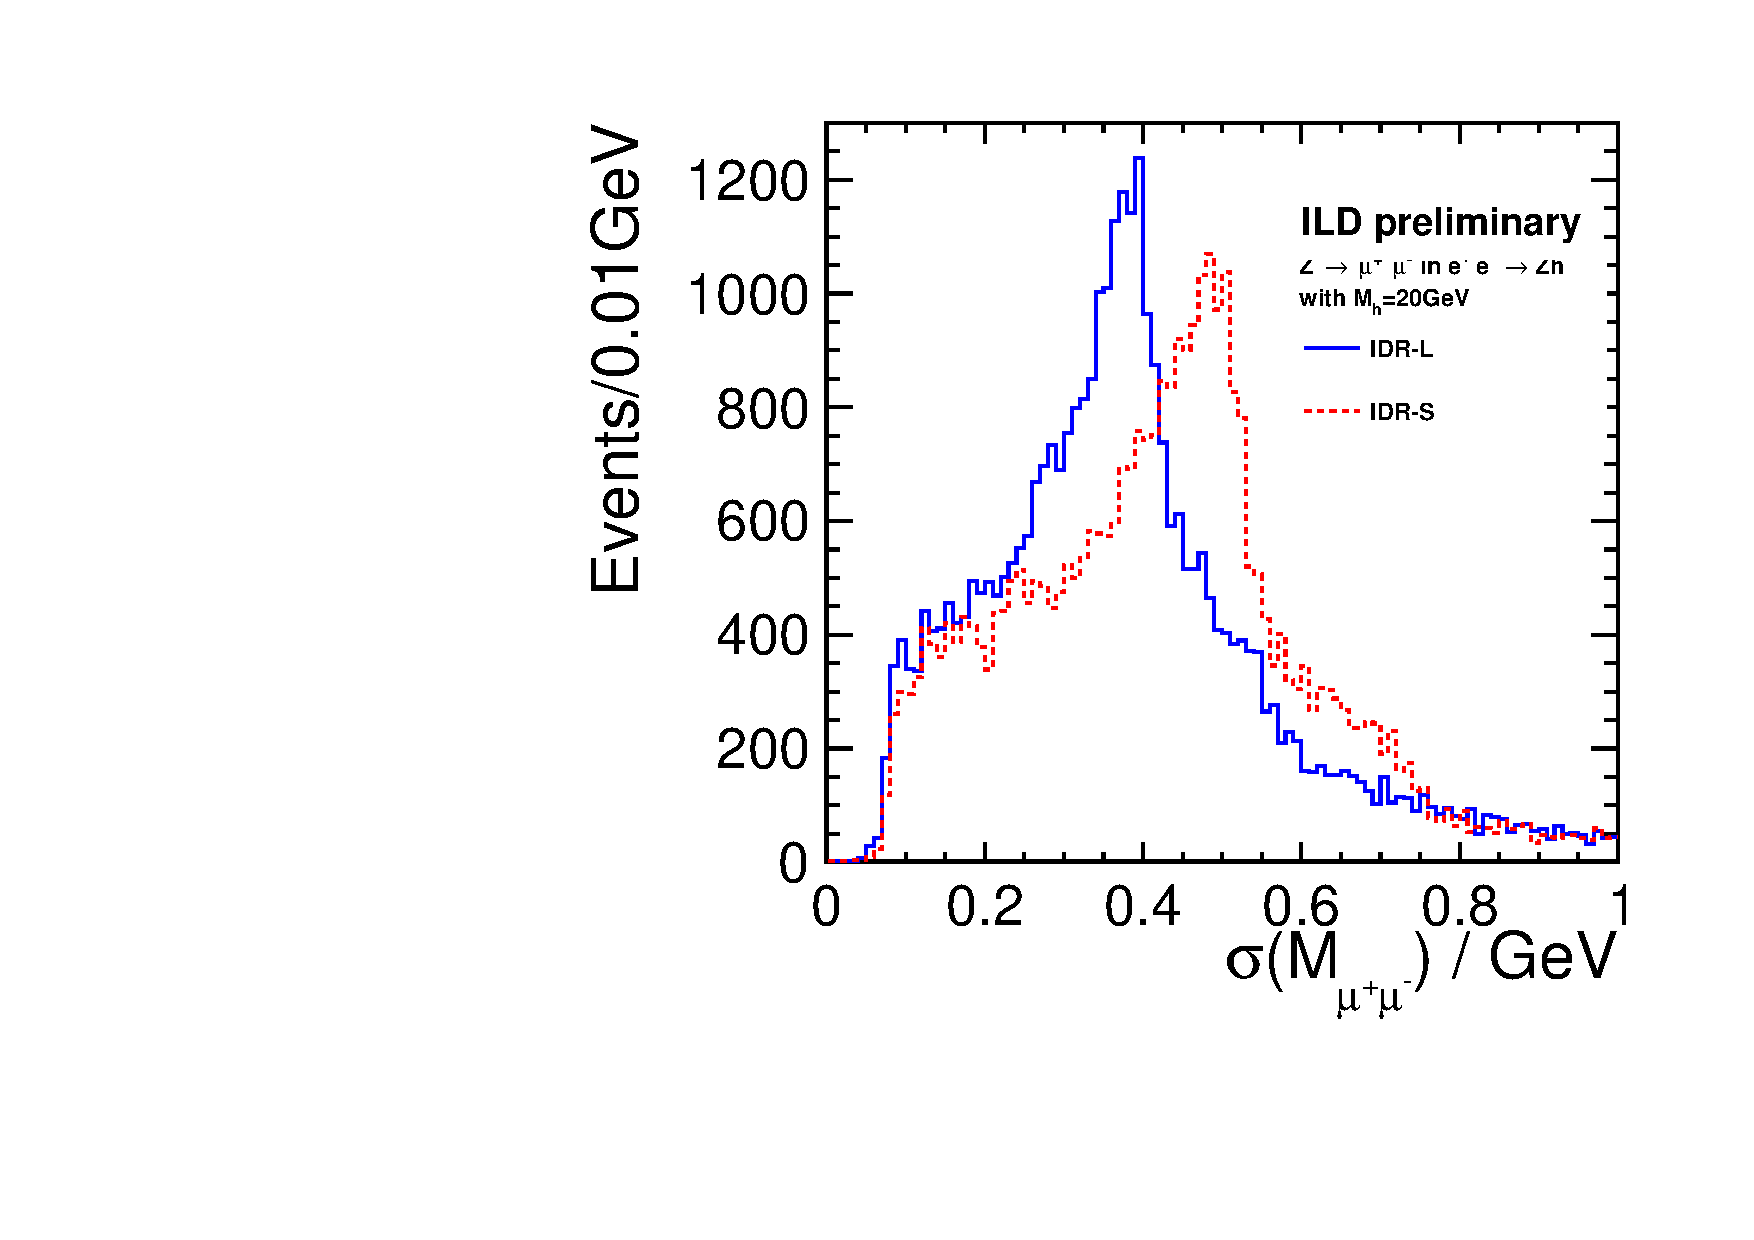
\includegraphics[width=\textwidth]{Performance/fig/lepton_pair_inm_sigma_nh20.pdf}
 \caption{ \label{fig:extraH:Msigma:mh20}}
 \end{subfigure}
%\hspace{0.03\textwidth}
\begin{subfigure}{0.475\hsize} 
\includegraphics[width=\textwidth]{Performance/fig/lepton_pair_inm_sigma_nh100.pdf}
 \caption{  \label{fig:extraH:Msigma:mh100}}
 \end{subfigure}
\begin{subfigure}{0.475\hsize} 
\includegraphics[width=\textwidth]{Performance/fig/lepton_pair_inm_sigma_nh300.pdf}
 \caption{ \label{fig:extraH:Msigma:mh300}}
 \end{subfigure}
%\hspace{0.03\textwidth}
\begin{subfigure}{0.475\hsize} 
\includegraphics[width=\textwidth]{Performance/fig/lepton_pair_inm_sigma_2f.pdf}
 \caption{  \label{fig:extraH:Msigma:2f}}
 \end{subfigure}
%\end{center}
\caption{Event-by-event uncertainty on the invariant di-muon mass calculated by error propagation from the track fit for different types of events sampling different ranges in polar angle and momentum of the muons in IDR-L and IDR-S:
(a) $ZS^0$ signal with $M_{S^0} = 20$\,GeV
(b) $ZS^0$ signal with $M_{S^0} = 100$\,GeV
(c) $ZS^0$ signal with $M_{S^0} = 300$\,GeV
(d) $2f$ background.
}
\label{fig:extraH:Msigma}
\end{figure}

% Figure~\ref{fig:extraH:ISRTagging} compares the performance of IDR-L and IDR-S in terms of the identification of ISR photons. \fix{[JL: at which level of the analysis is this plot made, and with which algorithm? Need documentation in note...]}
% 
% \begin{figure}[htbp]
% \begin{center} 
% \includegraphics[width=0.55\textwidth]{Performance/fig/ISRphoton_tagging_efficiency.pdf}
% \end{center}
% \caption{Performance of the ISR photon identification in IDR-L and IDR-S. True ISR photons are considered as signal, while the background comprises all PFOs identified as ISR photon, but having another true origin. \fix{[JL: improve plot layout]}}
% \label{fig:extraH:ISRTagging}
% \end{figure}

Figure~\ref{fig:extraH:limit:500} shows the resulting $95\%$ CL sensitivity of ILC500 as defined in Sec.~\ref{sec:benchmarks:lep} on the mixing of the new scalar with the SM-like Higgs boson, $\sin^2{\theta}$, as a function of the scalar mass $M_{S^0}$. Also shown is the corresponding observed limit by the OPAL collaboration~\cite{Abbiendi:2002qp}. Since the OPAL result is based on a combination of the $Z\to e^+e^-$ and $Z\to \mu^+\mu^-$ channels, the ILD projections have been scaled by a factor $1/\sqrt{2}$ to allow a more direct comparison. This assumes that the electron channel will reach a similar sensitivity than obtained for the case of muons, which is supported by the roughly similar performance of the two channels in the measurement of the total $ZH(125)$ cross section via the recoil technique~\cite{Yan:2016xyx}. 

No significant difference between IDR-L and IDR-S is observed at this level, since the effect of the beam energy spectrum covers the differences in momentum resolution. At low $M_{S^0}$, the performance reached with either IDR-L or IDR-S is somewhat worse than expected from the MC truth after hadronisation (``Pythia stable particle level'') due to imperfect recognition of ISR photons. Note that for scalar masses below about $150$\,GeV, the ILC run at $\sqrt{s}=250$\,GeV probes significantly smaller mixing angles $\sin^2{\theta}$, as can be seen in Fig.~\ref{fig:extraH:limit:250}. Also at $\sqrt{s}=250$\,GeV it has been observed that the detector performance matters most for $M_{S^0}<80$\,GeV, dominated by the ability (of the current reconstruction) to reconstruct and identify ISR photons~\cite{FIPnote:ESU_BSM}.

\begin{figure}[htbp]
\begin{center} 
\begin{subfigure}{0.49\hsize} 
 \includegraphics[width=\textwidth]{Performance/fig/exclusion_limits_08_03_compare_LEP.pdf}
 \caption{500\,GeV, IDR simulation\label{fig:extraH:limit:500}}
 \end{subfigure}
%\hspace{0.03\textwidth}
\begin{subfigure}{0.49\hsize} 
 \includegraphics[width=\textwidth]{Performance/fig/k95_250.pdf}
 \caption{250\,GeV, DBD simulation\label{fig:extraH:limit:250}}
 \end{subfigure}
\end{center}
\caption{Expected sensitivity of (a) ILC500 as defined in Sec.~\ref{sec:benchmarks:lep} at the $95\%$ CL for IDR-L and IDR-S compared to the existing limit from LEP~\cite{Abbiendi:2002qp}. (b) Corresponding result for the ILC run at $\sqrt{s}=250$\,GeV (2\,ab$^{-1}$, $|P(e^+,e^-)|=(30\%,80\%)$, $f(-+,+-,++,--) = (45\%,45\%, 5\%, 5\%)$), which probes significantly smaller mixing angles $\sin^2{\theta}$ for scalar masses below 140\,GeV~\cite{FIPnote:ESU_BSM}.
In both cases, the difference between the ``Pythia stable particle level'' (i.e.\ MC truth after hadronisation) and the full reconstruction results at small masses is mainly due to imperfect identification of ISR photons.}
\label{fig:extraH:limit}
\end{figure}



%%%%%%%%%%%%%%%%%%%%%%%%%%%%%%%%%%%%%%%%%%%%%%%%%%%%%%%%%%%%%%%%%%%
\subsection{Search for low \texorpdfstring{$\Delta M$}{DeltaM} Higgsinos}
\label{subsec:bench:higgsino}
%%%%%%%%%%%%%%%%%%%%%%%%%%%%%%%%%%%%%%%%%%%%%%%%%%%%%%%%%%%%%%%%%%%

New particles with at most electroweak interactions and small mass differences in the decay chain are among the prime examples of discovery opportunities at future $e^+e^-$ colliders. A prominent example of such kind of
new physics are higgsinos, which are expected to be light in natural SUSY models and tend to have small mass
splittings, in particular when the gaugino masses are much heavier. One of the model points studied previously in fast detector simulation~\cite{Berggren:2013vfa}, with a chargino mass of about 167\,GeV and a mass splitting of only $770$\,MeV between the chargino and the LSP, is used as a detector performance benchmark here~\cite{ILDNote:higgsinos}. For this mass splitting, the chargino decays to more than $99\%$ into a single charged particle and the LSP. Figure~\ref{fig:higgsino:trkeffi:pt} shows the transverse momentum ($p_t$) distribution of the charged particles in $e^+e^- \to \tilde{\chi}^+_1 \tilde{\chi}^-_1$ events at a center-of-mass energy of $500$\,GeV.

The tracking efficiency  as obtained in these events is displayed in Fig.~\ref{fig:higgsino:trkeffi:effi} as a function of the charged particle transverse momentum. 
For transverse
momenta below $p_t = 300$\,MeV, a clear difference can be seen between the two detector models due to the higher magnetic field of IDR-S. For this specific model point, which lies -- with $2 M(\tilde{\chi}^{\pm}_1) \approx 334$\,GeV -- significantly below the kinematic limit, the efficiency to detect all charged decay products is around $60$\% and differs only by $2$\% between IDR-L and IDR-S, thanks to the sufficient boost of the charginos. For chargino masses closer to the kinematic limit, however, the typical $p_t$ will be even lower, 
and the difference visible in Fig~\ref{fig:higgsino:trkeffi:effi} will lead to a larger effect.
The low $p_t$ tracking efficiency could be recovered at least partially by reducing the radii of the vertex detector layers for IDR-S, which is possible since the higher magnetic field also confines the pair background at smaller radii.
\begin{figure}[htbp]
\begin{center}
\begin{subfigure}{0.525\hsize} 
% plot from Swathi is *after* tracking efficiency has been applied!
%\includegraphics[width=\textwidth]{Performance/fig/pt_tracks_higgsinos.pdf}
\includegraphics[width=\textwidth]{Performance/fig/PT_genlevel_mh127_log.pdf}
 \caption{  \label{fig:higgsino:trkeffi:pt}}
\end{subfigure}
%\hspace{0.03\textwidth}
\begin{subfigure}{0.455\hsize} 
 \includegraphics[width=\textwidth]{Performance/fig/efficiency_higgsinos.pdf}
 \caption{ \label{fig:higgsino:trkeffi:effi}}
 \end{subfigure}
\end{center}
\caption{(a) Transverse momentum distribution of the visible decay products in the $\Delta M =770$\,MeV chargino sample (yellow) and in the corresponding neutralino sample (green) of the same SUSY benchmark at $\sqrt{s}=500$\,GeV~\cite{Berggren:2013vfa}. (b) Tracking efficiency obtained in IDR-L and IDR-S for the chargino decay products as a function of their transverse momentum.
}
\label{fig:higgsino:trkeffi}
\end{figure}


%%%%%%%%%%%%%%%%%%%%%%%%%%%%%%%%%%%%%%%%%%%%%%%%%%%%%%%%%%%%%%%%%%%
\subsection{WIMP Search in the Mono-Photon Channel}

%%%%%%%%%%%%%%%%%%%%%%%%%%%%%%%%%%%%%%%%%%%%%%%%%%%%%%%%%%%%%%%%%%%
The search for WIMP production via the mono-photon signature is another example of a search highly complementary to the HL-LHC, which predominantly probes couplings of WIMPs to quarks. This channel has been chosen as a  benchmark specifically in order to test the photon reconstruction and the performance of the BeamCAL, which plays an essential role in vetoing background from Bhabha scattering. The benchmark analysis is described in more detail in~\cite{ILDNote:WIMPs} and closely follows~\cite{Habermehl:2018yul}.
\begin{figure}[htbp]
%\begin{center}
\begin{subfigure}{0.49\hsize} 
\includegraphics[width=\textwidth]{Performance/fig/NrecNgenE_photon_IDR_wo_cosTheta08.pdf}
 \caption{ \label{fig:WIMP:Ngamma:Egood}}
 \end{subfigure}
%\hspace{0.03\textwidth}
\begin{subfigure}{0.49\hsize} 
\includegraphics[width=\textwidth]{Performance/fig/NrecNgenCosTheta_allpfo_IDR.pdf}
 \caption{  \label{fig:WIMP:NPFO:theta}}
 \end{subfigure}
% \begin{subfigure}{0.49\hsize} 
% \includegraphics[width=\textwidth]{Performance/fig/NrecNgenE_photon_IDR.pdf}
%  \caption{ \label{fig:WIMP:Ngamma:E}}
%  \end{subfigure}
% %\hspace{0.03\textwidth}
% \begin{subfigure}{0.49\hsize} 
% \includegraphics[width=\textwidth]{Performance/fig/NrecNgenCosTheta_photon_IDR.pdf}
%  \caption{  \label{fig:WIMP:Ngamma:theta}}
%  \end{subfigure}
%\end{center}
\caption{Ratio of recontructed and generated PFOs per $\nu\nu\gamma$ event for ILC500 as defined in Sec.~\ref{sec:benchmarks:lep}
(a) based on PFOs identified as photons as function of the photon energy, excluding the corner region between barrel and endcap ($|\cos{\theta}|\simeq 0.8$)
(b) based on all PFOs as function of the photon polar angle.}

%(c) based on PFOs identified as photons as function of the photon energy
%(d) based PFOs identified as photons as function of the photon polar angle. 
%}
\label{fig:WIMP:Ngamma}
\end{figure}

Figure~\ref{fig:WIMP:Ngamma} shows the ratio of reconstructed and generated photons per $\nu\nu\gamma$ event as a function of
the photon's energy and polar angle. While it has been shown in~\cite{Habermehl:2018yul} that the actual energy
resolution is not very critical in this analysis, it is important that the number of photons is correct, since the signature of a single photon and no other significant detector activity forms the basis of the selection.
As can be seen in Fig.~\ref{fig:WIMP:Ngamma:Egood}, the average number of reconstructed photons per generated photon tends to be a few permille below 1 at low photon energies. With increasing photon energy, the tendency of the particle flow reconstruction to split a photon into two increases, but stays below the level of 1\% for IDR-L and below 2\% for IDR-S. In both cases, the corner region between barrel and endcap has been excluded, because the current reconstruction software tends to split PFOs in this region. This can be clearly seen in 
Fig.~\ref{fig:WIMP:NPFO:theta} which shows the ratio of reconstructed PFOs vs generated particles as a function of $\cos{\theta}$. Also indicated are the locations of the barrel-endcap transition for IDR-L and IDR-S, which occurs at different polar angles due to the different aspect ratios of the two detector models.  All the features in these two plots are expected to be reducable with further development of the particle flow reconstruction.

\begin{figure}[htbp]
%\begin{center}
\begin{subfigure}{0.49\hsize} 
%\includegraphics[width=\textwidth]{Performance/fig/bcalveto_IDR-L.pdf}
\includegraphics[width=\textwidth]{Performance/fig/bcalveto_vv1g_comp.pdf}
 \caption{$\nu\bar{\nu}\gamma$ \label{fig:WIMP:BCal:IDR-L}}
 \end{subfigure}
%\hspace{0.03\textwidth}
\begin{subfigure}{0.49\hsize} 
%\includegraphics[width=\textwidth]{Performance/fig/bcalveto_IDR-S.pdf}
\includegraphics[width=\textwidth]{Performance/fig/bcalveto_eeNg_comp.pdf}
\caption{$e^+e^- N\gamma$ \label{fig:WIMP:BCal:IDR-S}}
 \end{subfigure}
%\end{center}
\caption{Number of BeamCAL clusters reconstructed in radiative neutrino and radiative Bhabha events for IDR-L and IDR-S, for ILC500 as defined in Sec.~\ref{sec:benchmarks:lep}. No significant difference between the detector models is observed.
}
\label{fig:WIMP:BCal}
\end{figure}

Figure~\ref{fig:WIMP:BCal} compares the number of reconstructed clusters in the BeamCal of the two detector models. Ideally, the $\nu\bar{\nu}\gamma$ events, which serve as proxy for the WIMP signal, should have no BeamCal cluster, while for the majority of the $e^+e^-\gamma$ events at least one BeamCal cluster should be found. Events with at least one cluster in the BeamCal will be rejected in the analysis. Due to its higher $B$ field, the background from $e^+e^-$ pairs is confined to somewhat smaller radii in case of IDR-S. This, however, does not lead to a significant effect on the number of reconstructed clusters in the BeamCal.

\begin{figure}[htbp]
\begin{center}
\begin{subfigure}{0.49\hsize} 
 \includegraphics[width=\textwidth]{Performance/fig/sensitivity_H20_IDR.pdf}
 \caption{linear mass scale\label{fig:WIMP:limit:std}}
 \end{subfigure}
%\hspace{0.03\textwidth}
\begin{subfigure}{0.49\hsize} 
 \includegraphics[width=\textwidth]{Performance/fig/sensitivity_H20_IDR_logx.pdf}
 \caption{logarithmic mass scale\label{fig:WIMP:limit:lowM}}
 \end{subfigure}
\end{center}
\caption{Expected sensitivity of ILC500 as defined in Sec.~\ref{sec:benchmarks:lep} at $95$\% CL in the plane of the new physics scale $\Lambda$ vs the WIMP mass $M_{\chi}$ for the cases of a vector, axial-vector or scalar operator describing the WIMP-SM interaction.}
\label{fig:WIMP:limit}
\end{figure}

The final result of the analysis is compared in Fig.~\ref{fig:WIMP:limit:std} for the two detector models for scalar, vector, and axial-vector operators for WIMP masses down to $1$\,GeV. At this level, no difference between IDR-L and IDR-S is perceivable. Figure~\ref{fig:WIMP:limit:lowM} extends the projection down to masses of $1$\,eV in order to illustrate the sensitivity to light feably interacting particles.

